% !TEX program = xelatex
\documentclass[a4paper]{article}
\nonstopmode
\usepackage[fontsize=13pt]{fontsize}
\usepackage[a4paper,left=3cm,right=1.5cm,top=2cm,bottom=2cm]{geometry}
\usepackage{fontspec}
\IfFontExistsTF{Times New Roman}{\setmainfont{Times New Roman}[Ligatures=TeX]\setsansfont{Times New Roman}[Ligatures=TeX]}{\setmainfont{Tinos}[Ligatures=TeX]\setsansfont{Tinos}[Ligatures=TeX]}
\IfFontExistsTF{Courier New}{\setmonofont{Courier New}[Scale=MatchLowercase]}{\setmonofont{DejaVu Sans Mono}[Scale=MatchLowercase]}
\usepackage{setspace}
\onehalfspacing
\usepackage{indentfirst}
\setlength{\parindent}{1.27cm}
\setlength{\parskip}{4pt}
\sloppy
\emergencystretch=3em
\usepackage{graphicx}
\usepackage{float}
\usepackage{longtable,booktabs,array,calc}
\usepackage{caption}
\usepackage{enumitem}
\usepackage{xurl}
\usepackage{hyperref}
\hypersetup{unicode=true,colorlinks=true,linkcolor=black,citecolor=blue}
\usepackage{bookmark}
\usepackage{fancyhdr}
\usepackage{titlesec}
\usepackage{listings}
\usepackage{xcolor}
\usepackage{eso-pic}
\newcommand{\coverframe}{\AddToShipoutPictureBG*{\AtPageLowerLeft{\put(\LenToUnit{1.3cm},\LenToUnit{1.3cm}){\framebox(\LenToUnit{\paperwidth-2.6cm},\LenToUnit{\paperheight-2.6cm}){}}}}}
\newcolumntype{L}[1]{>{\raggedright\arraybackslash}p{#1}}
\newcolumntype{C}[1]{>{\centering\arraybackslash}p{#1}}
\setlist[itemize]{leftmargin=1.1cm,itemsep=0.12em,topsep=0.15em}
\setlist[enumerate]{leftmargin=1.1cm,itemsep=0.12em,topsep=0.15em}
\urlstyle{same}
\captionsetup[figure]{labelsep=period,font=normalsize,justification=centering,singlelinecheck=false}
\captionsetup[table]{labelsep=period,font=normalsize,justification=raggedright,singlelinecheck=false}
\newcounter{chapnum}
\renewcommand{\thefigure}{\arabic{chapnum}.\arabic{figure}}
\renewcommand{\thetable}{\arabic{chapnum}.\arabic{table}}
\renewcommand{\theHfigure}{\arabic{chapnum}.\arabic{figure}}
\renewcommand{\theHtable}{\arabic{chapnum}.\arabic{table}}
\renewcommand{\contentsname}{MỤC LỤC}
\renewcommand{\listfigurename}{DANH MỤC HÌNH ẢNH}
\renewcommand{\listtablename}{DANH MỤC BẢNG BIỂU}
\renewcommand{\figurename}{Hình}
\renewcommand{\tablename}{Bảng}
\setcounter{tocdepth}{3}
\titleformat{\section}{\normalfont\bfseries\centering\fontsize{14pt}{18pt}\selectfont}{}{0pt}{}
\titleformat{\subsection}{\normalfont\bfseries\fontsize{13pt}{16pt}\selectfont}{}{0pt}{}
\titleformat{\subsubsection}{\normalfont\bfseries\fontsize{13pt}{16pt}\selectfont}{}{0pt}{}
\titlespacing*{\section}{0pt}{0.8cm}{0.45cm}
\titlespacing*{\subsection}{0pt}{0.45cm}{0.25cm}
\titlespacing*{\subsubsection}{0pt}{0.35cm}{0.2cm}
\pagestyle{fancy}
\fancyhf{}
\fancyhead[R]{\textit{Đồ án tốt nghiệp}}
\fancyhead[C]{\thepage}
\renewcommand{\headrulewidth}{0pt}
\renewcommand{\footrulewidth}{0pt}
\setlength{\headheight}{17pt}
\fancypagestyle{plain}{\fancyhf{}\fancyhead[R]{\textit{Đồ án tốt nghiệp}}\fancyhead[C]{\thepage}\renewcommand{\headrulewidth}{0pt}\renewcommand{\footrulewidth}{0pt}}
\lstset{basicstyle=\ttfamily\small,breaklines=true,frame=single,columns=fullflexible}
\renewcommand{\arraystretch}{1.25}
\newcommand{\chap}[1]{\clearpage\section*{#1}\phantomsection\addcontentsline{toc}{section}{#1}}
\newcommand{\secx}[1]{\subsection*{#1}\phantomsection\addcontentsline{toc}{subsection}{#1}}
\newcommand{\subsecx}[1]{\subsubsection*{#1}\phantomsection\addcontentsline{toc}{subsubsection}{#1}}
\newcommand{\imgfig}[2]{\begin{figure}[H]\centering\includegraphics[width=0.95\textwidth,keepaspectratio]{#1}\caption{#2}\end{figure}}
\newcommand{\smallimgfig}[2]{\begin{figure}[H]\centering\includegraphics[width=0.70\textwidth,keepaspectratio]{#1}\caption{#2}\end{figure}}

\begin{document}
\pagenumbering{roman}

% Bìa (Phụ lục 3)
\begin{titlepage}
\thispagestyle{empty}
\coverframe
\begin{center}
{\fontsize{14pt}{18pt}\selectfont\bfseries BỘ GIÁO DỤC VÀ ĐÀO TẠO}\\[0.15cm]
{\fontsize{14pt}{18pt}\selectfont\bfseries TRƯỜNG ĐẠI HỌC TÂN TẠO}\\[1.0cm]
\IfFileExists{media/ttu_logo.png}{
\includegraphics[width=4.6cm]{media/ttu_logo.png}}{\vspace{2.3cm}}\\[1.4cm]
{\fontsize{15pt}{19pt}\selectfont\bfseries Võ Hữu Nhân}\\[0.15cm]
{\fontsize{15pt}{19pt}\selectfont\bfseries MSSV: 2202083}\\[0.15cm]
{\fontsize{15pt}{19pt}\selectfont\bfseries Khóa: 2022 - 2026}\\[1.3cm]
{\fontsize{15pt}{19pt}\selectfont\bfseries NGHIÊN CỨU VÀ XÂY DỰNG HỆ THỐNG TÁC NHÂN TỰ CHỦ HỖ TRỢ VẬN HÀNH MARKETING SỐ}\\[0.9cm]
{\fontsize{14pt}{18pt}\selectfont\bfseries ĐỒ ÁN TỐT NGHIỆP CỬ NHÂN KHOA HỌC MÁY TÍNH}
\end{center}
\vfill
\begin{center}
{\fontsize{14pt}{18pt}\selectfont\bfseries TÂY NINH -- THÁNG 6 NĂM 2026}
\end{center}
\end{titlepage}

\clearpage

% Trang phụ bìa (Phụ lục 4)
\begin{titlepage}
\thispagestyle{empty}
\coverframe
\begin{center}
{\fontsize{14pt}{18pt}\selectfont\bfseries BỘ GIÁO DỤC VÀ ĐÀO TẠO}\\[0.15cm]
{\fontsize{14pt}{18pt}\selectfont\bfseries TRƯỜNG ĐẠI HỌC TÂN TẠO}\\[1.8cm]
{\fontsize{15pt}{19pt}\selectfont\bfseries Võ Hữu Nhân}\\[0.15cm]
{\fontsize{15pt}{19pt}\selectfont\bfseries MSSV: 2202083}\\[0.15cm]
{\fontsize{15pt}{19pt}\selectfont\bfseries Khóa: 2022 - 2026}\\[1.3cm]
{\fontsize{15pt}{19pt}\selectfont\bfseries NGHIÊN CỨU VÀ XÂY DỰNG HỆ THỐNG TÁC NHÂN TỰ CHỦ HỖ TRỢ VẬN HÀNH MARKETING SỐ}\\[0.7cm]
Ngành: Khoa học máy tính\\[0.1cm]
Mã số: 7480101\\[0.7cm]
{\fontsize{14pt}{18pt}\selectfont\bfseries ĐỒ ÁN TỐT NGHIỆP CỬ NHÂN KHOA HỌC MÁY TÍNH}\\[1.3cm]
\emph{Giảng viên hướng dẫn khoa học: TS. Cao Tiến Dũng}\\[0.1cm]
\emph{(Chữ ký)}\\[1.6cm]
{\fontsize{14pt}{18pt}\selectfont\bfseries TS. Cao Tiến Dũng}
\end{center}
\vfill
\begin{center}
{\fontsize{14pt}{18pt}\selectfont\bfseries TÂY NINH -- THÁNG 6 NĂM 2026}
\end{center}
\end{titlepage}

\clearpage
\section*{TRANG PHÊ DUYỆT}
Đồ án đã được trình và bảo vệ trước Hội đồng chấm đồ án tốt nghiệp.

\vspace{0.4cm}
\textbf{Ngày bảo vệ:} ....../....../20......

\textbf{Kết quả:} ....../10 điểm

\vspace{2cm}
\noindent
\begin{tabular}{C{0.47\textwidth}C{0.47\textwidth}}
\textbf{GIẢNG VIÊN HƯỚNG DẪN} & \textbf{GIẢNG VIÊN PHẢN BIỆN}\\[0.2cm]
\emph{(Ký và ghi rõ họ tên)} & \emph{(Ký và ghi rõ họ tên)}\\[3cm]
\end{tabular}
\vspace{1cm}
\begin{center}
\textbf{CHỦ TỊCH HỘI ĐỒNG}\\[0.2cm]
\emph{(Ký và ghi rõ họ tên)}
\end{center}

\clearpage
\section*{LỜI CAM ĐOAN}\phantomsection\addcontentsline{toc}{section}{LỜI CAM ĐOAN}
\textbf{\emph{Tôi xin cam đoan đây là công trình nghiên cứu của riêng tôi. Các số liệu, kết quả trong đề tài là trung thực và chưa từng được công bố trong bất kỳ công trình nào.}}

\begin{flushright}
\textbf{Tác giả đồ án}\\
\emph{(ký và ghi rõ họ tên)}
\end{flushright}

\clearpage
\section*{LỜI CẢM ƠN}\phantomsection\addcontentsline{toc}{section}{LỜI CẢM ƠN}
Trước hết, em xin chân thành cảm ơn Khoa Công nghệ thông tin, Trường Đại học Tân Tạo đã tạo điều kiện cho em trong quá trình học tập và thực hiện đồ án tốt nghiệp.

Em xin cảm ơn Thầy Cao Tiến Dũng đã hướng dẫn, góp ý và giúp em xác định phạm vi đề tài. Trong quá trình làm đồ án, những góp ý của Thầy giúp em nhìn rõ hơn phần nào là chức năng chính, phần nào là thành phần kỹ thuật nền và phần nào chỉ nên để ở hướng phát triển.

Em cũng xin cảm ơn quý thầy cô trong Khoa Công nghệ thông tin đã truyền đạt cho em các kiến thức nền tảng về lập trình, hệ thống phần mềm, trí tuệ nhân tạo, cơ sở dữ liệu và kiểm thử phần mềm. Đây là những kiến thức cần thiết để em có thể phân tích, thiết kế và hiện thực hệ thống trong đồ án.

Cuối cùng, em xin cảm ơn gia đình, bạn bè và những người đã động viên em trong suốt quá trình học tập. Do thời gian và kinh nghiệm còn hạn chế, đồ án chắc chắn vẫn còn thiếu sót. Em mong nhận được góp ý của quý thầy cô để có thể tiếp tục hoàn thiện hệ thống sau này.

Em xin chân thành cảm ơn!

\clearpage
\section*{TÓM TẮT ĐỒ ÁN}
\phantomsection
\addcontentsline{toc}{section}{TÓM TẮT ĐỒ ÁN}

Trong hoạt động marketing số, cá nhân, nhà sáng tạo nội dung và doanh nghiệp nhỏ thường phải xử lý nhiều công việc lặp lại như phân tích yêu cầu, tìm hiểu thị trường, lập kế hoạch truyền thông, viết nội dung, chỉnh sửa nội dung theo nền tảng, theo dõi lịch công việc và tổng hợp báo cáo. Khi các công việc này được thực hiện rời rạc trên nhiều công cụ khác nhau, người dùng dễ mất thời gian, khó theo dõi tiến độ và khó duy trì sự nhất quán về thông tin thương hiệu.

Đồ án này nghiên cứu và xây dựng một hệ thống tác nhân tự chủ hỗ trợ vận hành marketing số. Hệ thống được phát triển dựa trên một nền tảng tác nhân có sẵn, sau đó được phân tích, tùy biến và bổ sung theo bài toán marketing. Trong phạm vi đồ án, hệ thống hỗ trợ các chức năng như phân tích yêu cầu marketing, hỗ trợ nghiên cứu thị trường và đối thủ, lập kế hoạch truyền thông, tạo bản nháp nội dung marketing, tạo biến thể và chỉnh sửa nội dung, lập lịch và tạo tác vụ định kỳ, tạo báo cáo marketing, hỗ trợ phân tích số liệu quảng cáo ở mức tham khảo và hỗ trợ phối hợp nhóm trong quá trình vận hành marketing.

Các chức năng của hệ thống được triển khai theo hướng hỗ trợ người dùng tạo bản nháp, gợi ý phương án và tổng hợp thông tin phục vụ công việc marketing. Đối với các thao tác có ảnh hưởng trực tiếp ra bên ngoài như đăng bài, gửi tin nhắn hàng loạt, chỉnh sửa chiến dịch hoặc thay đổi ngân sách quảng cáo, hệ thống không tự động thực hiện nếu chưa có sự kiểm tra và phê duyệt của người dùng. Cách tiếp cận này giúp hệ thống có thể hỗ trợ công việc lặp lại nhưng vẫn giữ vai trò kiểm soát cuối cùng cho người dùng.

Kết quả của đồ án là một hệ thống có thể chạy thử nghiệm và hỗ trợ các chức năng chính đã xác định trong phạm vi đề tài. Hệ thống được kiểm tra thông qua các kịch bản sử dụng giả lập như phân tích yêu cầu marketing, lập kế hoạch truyền thông, tạo nội dung, chỉnh sửa nội dung theo nền tảng, tạo tác vụ định kỳ, tổng hợp báo cáo và kiểm soát các thao tác cần phê duyệt. Trong đó, phần chức năng marketing do đồ án tự xây dựng được kiểm thử bằng 61 testcase, bên cạnh 247 testcase thuộc các thành phần nền được kế thừa. Kết quả kiểm thử cho thấy hệ thống đáp ứng được mục tiêu xây dựng một tác nhân tự chủ hỗ trợ vận hành marketing số ở mức nền tảng.

\textbf{Từ khóa:} tác nhân tự chủ, mô hình ngôn ngữ lớn, marketing số, vận hành marketing, bản nháp nội dung, tác vụ định kỳ.


\clearpage
\section*{ABSTRACT}
\phantomsection
\addcontentsline{toc}{section}{ABSTRACT}

In digital marketing activities, individuals, content creators, and small businesses often have to handle many repetitive tasks such as requirement analysis, market research, communication planning, content writing, platform-based content editing, task tracking, and report summarization. When these tasks are handled separately across different tools, users may spend more time managing work, find it difficult to track progress, and struggle to maintain consistency in brand information.

This project studies and develops an autonomous agent system to support digital marketing operations. The system is developed based on an existing agent platform, which is then analyzed, customized, and extended for the marketing use case. Within the scope of this project, the system supports functions such as marketing requirement analysis, market and competitor research support, communication planning, marketing draft generation, content variation and editing, scheduled task creation, marketing report generation, advertising data analysis at a support level, and team collaboration support in marketing operations.

The system functions are implemented with the goal of helping users create drafts, receive suggestions, and summarize information for marketing tasks. For actions that may directly affect external systems, such as publishing posts, sending bulk messages, modifying campaigns, or changing advertising budgets, the system does not execute them automatically without user review and approval. This approach allows the system to support repetitive work while keeping the user in control of important decisions.

The result of the project is a system that can be run experimentally and support the main functions defined within the project scope. The system is tested through simulated usage scenarios such as marketing requirement analysis, communication planning, content generation, platform-based content editing, scheduled task creation, report summarization, and control of actions that require approval. The marketing functions built specifically for this project are verified by 61 test cases, alongside 247 test cases covering the inherited foundational components. The testing results show that the system meets the objective of building a foundational autonomous agent system to support digital marketing operations.

\textbf{Keywords:} autonomous agent, large language model, digital marketing, marketing operations, marketing drafts, scheduled tasks.


\clearpage
\phantomsection\addcontentsline{toc}{section}{MỤC LỤC}
\tableofcontents

\clearpage
\phantomsection\addcontentsline{toc}{section}{DANH MỤC HÌNH ẢNH}
\listoffigures

\clearpage
\phantomsection\addcontentsline{toc}{section}{DANH MỤC BẢNG BIỂU}
\listoftables

\clearpage

\section*{DANH MỤC TỪ VIẾT TẮT}\phantomsection\addcontentsline{toc}{section}{DANH MỤC TỪ VIẾT TẮT}
\begingroup
\renewcommand{\theHtable}{frontabbr}
\begin{longtable}{L{0.20\textwidth}L{0.70\textwidth}}
\toprule
\textbf{Từ viết tắt} & \textbf{Giải thích}\\
\midrule
\endfirsthead
\toprule
\textbf{Từ viết tắt} & \textbf{Giải thích}\\
\midrule
\endhead
AI & Trí tuệ nhân tạo (Artificial Intelligence).\\
API & Giao diện lập trình ứng dụng, dùng để các phần mềm trao đổi dữ liệu hoặc gọi chức năng của nhau.\\
CLI & Giao diện dòng lệnh, nơi người dùng nhập lệnh để chạy hệ thống.\\
JSON & Định dạng dữ liệu dạng văn bản, thường dùng để lưu cấu hình hoặc dữ liệu có cấu trúc.\\
JSONL & Định dạng lưu nhiều bản ghi JSON theo từng dòng, phù hợp với Transcript hoặc nhật ký chạy tác vụ.\\
KPI & Chỉ số đánh giá hiệu quả công việc hoặc chiến dịch.\\
LLM & Mô hình ngôn ngữ lớn, dùng để hiểu yêu cầu và sinh nội dung.\\
RAG & Retrieval-Augmented Generation, kỹ thuật truy xuất thông tin liên quan trước khi mô hình ngôn ngữ sinh câu trả lời.\\
SDK & Bộ công cụ phát triển phần mềm.\\
UI & Giao diện người dùng.\\
\bottomrule
\end{longtable}
\endgroup

\clearpage
\section*{DANH MỤC THUẬT NGỮ}\phantomsection\addcontentsline{toc}{section}{DANH MỤC THUẬT NGỮ}
\begingroup
\renewcommand{\theHtable}{frontterms}
\begin{longtable}{L{0.30\textwidth}L{0.60\textwidth}}
\toprule
\textbf{Thuật ngữ} & \textbf{Giải thích}\\
\midrule
\endfirsthead
\toprule
\textbf{Thuật ngữ} & \textbf{Giải thích}\\
\midrule
\endhead
Agent Runtime & Thành phần trung tâm nhận yêu cầu, chuẩn bị ngữ cảnh, gọi mô hình, điều phối công cụ và lưu kết quả.\\
Approval & Bản ghi yêu cầu phê duyệt cho các hành động nhạy cảm như đăng bài, gửi tin hàng loạt hoặc thao tác quảng cáo.\\
Autonomous Agent & Hệ thống có khả năng tiếp nhận mục tiêu, phân tích ngữ cảnh, chọn bước xử lý và sử dụng công cụ trong phạm vi cho phép.\\
Brand & Thông tin thương hiệu được lưu có cấu trúc: giọng văn, định vị, khách hàng mục tiêu, trụ cột thông điệp và ràng buộc nội dung.\\
Brand Context & Thông tin về thương hiệu, sản phẩm, khách hàng mục tiêu, giọng văn, thông điệp và ràng buộc nội dung.\\
Campaign & Thông tin một chiến dịch: tóm tắt yêu cầu, kênh dự kiến, chỉ số đo lường, ràng buộc và mốc thời gian.\\
Capability Layer & Lớp chứa công cụ, plugin, Model Provider, plugin Memory và Channel Adapter.\\
Channel Adapter & Thành phần chuẩn hóa dữ liệu đầu vào và đầu ra giữa hệ thống với các kênh giao tiếp.\\
Client Layer & Lớp nơi người dùng gửi yêu cầu và nhận kết quả qua CLI, giao diện web hoặc kênh nhắn tin.\\
ContentPlan & Kế hoạch nội dung của một chiến dịch, gồm nhiều khung nội dung theo thời điểm, kênh và định dạng.\\
Context Assembly & Bước tổng hợp yêu cầu hiện tại, Session, Workspace và Memory liên quan trước khi gửi vào mô hình.\\
Context Engine & Thành phần hỗ trợ chuẩn bị, bảo trì và rút gọn ngữ cảnh của Session.\\
Gateway Runtime & Thành phần tiếp nhận dữ liệu từ các kênh, chuẩn hóa yêu cầu và chuyển vào Agent Runtime.\\
Human-in-the-loop & Cơ chế giữ người dùng trong vòng quyết định đối với các hành động có ảnh hưởng ra bên ngoài.\\
Insight & Nhận xét hoặc bài học rút ra từ các lần làm việc trước, được lưu lại để sử dụng lại về sau.\\
Lead & Thông tin khách hàng tiềm năng cùng trạng thái theo dõi.\\
marketing store & Lớp dữ liệu marketing có cấu trúc, chứa các mục như Brand, Product, Campaign, ContentPlan, PostDraft, Approval, Insight và Lead.\\
Memory Retrieval & Quá trình tìm thông tin liên quan trong Memory để hỗ trợ xử lý yêu cầu hiện tại.\\
Model Provider & Thành phần hoặc dịch vụ cung cấp mô hình ngôn ngữ lớn cho hệ thống.\\
Model Router & Thành phần chọn Model Provider và mô hình cần dùng theo cấu hình hoặc cơ chế dự phòng.\\
Plugin System & Cách mở rộng hệ thống bằng các gói bổ sung công cụ, Model Provider, Memory hoặc kênh giao tiếp.\\
PostDraft & Bản nháp bài đăng cho một kênh nhất định, có vòng đời trạng thái từ ý tưởng đến khi được phê duyệt, lập lịch, xuất bản và đo lường.\\
Product & Thông tin sản phẩm: mô tả, tính năng, lợi ích, điểm bán hàng độc nhất và câu hỏi thường gặp.\\
Retrieval-Augmented Generation & Kỹ thuật kết hợp mô hình ngôn ngữ với thông tin được truy xuất từ nguồn dữ liệu bên ngoài, thường viết tắt là RAG.\\
Scheduler & Thành phần tạo và chạy nhắc việc, báo cáo hoặc tác vụ định kỳ.\\
SecretRef & Cách lưu tham chiếu đến thông tin xác thực thay vì đưa trực tiếp khóa bí mật vào prompt hoặc Transcript.\\
Session & Cơ chế tách riêng ngữ cảnh theo người dùng, kênh giao tiếp, luồng hội thoại hoặc tác vụ định kỳ.\\
Storage Layer & Lớp lưu cấu hình, Transcript, Memory, lịch tác vụ, nhật ký chạy và tham chiếu bí mật.\\
Subagent Runtime & Tác nhân con hỗ trợ chia một yêu cầu lớn thành các phần nhỏ hơn để xử lý song song.\\
Tool Policy & Quy tắc quyết định công cụ nào được phép dùng trong từng lượt chạy.\\
Tool Registry & Nơi quản lý các công cụ mà tác nhân có thể sử dụng.\\
Transcript & Nhật ký lưu các lượt trao đổi, lời gọi công cụ và kết quả công cụ trong một Session.\\
Workspace & Không gian chứa cấu hình, hướng dẫn và các tệp liên quan đến quá trình vận hành hệ thống.\\
\bottomrule
\end{longtable}
\endgroup

\clearpage
\pagenumbering{arabic}

\setcounter{chapnum}{1}
\setcounter{figure}{0}
\setcounter{table}{0}
\chap{CHƯƠNG 1: GIỚI THIỆU}
\secx{1.1. Đặt vấn đề}
Marketing số hiện nay không chỉ là viết một bài quảng cáo rồi đăng lên mạng xã hội. Một người làm marketing thường phải hiểu sản phẩm, xác định khách hàng mục tiêu, chuẩn bị thông điệp, lập kế hoạch nội dung, chỉnh sửa nội dung theo từng nền tảng, theo dõi phản hồi và tổng hợp báo cáo. Với cá nhân, nhà sáng tạo nội dung, cửa hàng nhỏ hoặc nhóm marketing ít nhân sự, các công việc này dễ bị lặp lại và tốn nhiều thời gian.

Trong thực tế, một chiến dịch nhỏ cũng có thể cần nhiều loại đầu ra khác nhau như bài đăng Facebook, kịch bản video ngắn, email, nội dung quảng cáo hoặc báo cáo ngắn. Nếu mỗi lần làm người dùng phải nhập lại thông tin sản phẩm, giọng văn, khách hàng mục tiêu và các ràng buộc nội dung thì quá trình làm việc sẽ bị chậm và dễ thiếu nhất quán. Vì vậy, bài toán không chỉ là tạo nội dung, mà còn là duy trì ngữ cảnh làm việc và hỗ trợ người dùng xử lý nhiều bước marketing một cách có kiểm soát.

Mô hình ngôn ngữ lớn có thể hỗ trợ tốt các tác vụ ngôn ngữ như phân tích yêu cầu, viết nháp, tóm tắt và chuyển đổi văn phong. Tuy nhiên, nếu chỉ dùng mô hình như một chatbot riêng lẻ, hệ thống thường không có bộ nhớ dài hạn, không quản lý phiên rõ ràng và khó kiểm soát khi cần dùng công cụ. Các nghiên cứu về LLM agent cho thấy một hệ thống tác nhân thường cần kết hợp mô hình ngôn ngữ với bộ nhớ, công cụ, lập lịch và chính sách an toàn \cite{ref1}, \cite{ref2}. Đây là hướng phù hợp để xây dựng hệ thống hỗ trợ vận hành marketing số.

Từ những lý do trên, nên tôi lựa chọn đề tài đồ án là ``Nghiên cứu và xây dựng hệ thống tác nhân tự chủ hỗ trợ vận hành marketing số''. Đồ án không đặt mục tiêu xây dựng một nền tảng marketing hoàn chỉnh thay thế con người. Thay vào đó, đồ án tập trung nghiên cứu, tùy biến và phát triển một hệ thống tác nhân dựa trên nền tảng có sẵn để hỗ trợ một số công việc phổ biến trong vận hành marketing số. Các hành động có thể gây ảnh hưởng ra bên ngoài như đăng bài, thay đổi ngân sách quảng cáo vẫn cần có sự kiểm tra và phê duyệt của người dùng.

\secx{1.2. Mục tiêu nghiên cứu}

\subsecx{1.2.1. Mục tiêu tổng quát}

Mục tiêu tổng quát của đề tài là nghiên cứu, tùy biến và phát triển một hệ thống tác nhân tự chủ nhằm hỗ trợ vận hành marketing số. Hệ thống tập trung hỗ trợ các công việc như phân tích yêu cầu marketing, nghiên cứu thị trường và đối thủ ở mức hỗ trợ, lập kế hoạch truyền thông, tạo bản nháp nội dung, tạo và chỉnh sửa nội dung phù hợp với từng nền tảng, lập lịch tác vụ định kỳ, tạo báo cáo marketing, phân tích số liệu quảng cáo ở mức tham khảo và hỗ trợ phối hợp nhóm trong quá trình vận hành marketing.

Hệ thống hướng đến việc giảm bớt một số công việc lặp lại trong quá trình làm marketing, đồng thời giúp người dùng có thêm công cụ hỗ trợ khi lập kế hoạch, tạo nội dung, theo dõi công việc và tổng hợp thông tin.

\subsecx{1.2.2. Mục tiêu cụ thể}

Các mục tiêu cụ thể của đề tài gồm:

\begin{itemize}
\item Tìm hiểu các kiến thức nền tảng liên quan đến marketing số, mô hình ngôn ngữ lớn và hệ thống tác nhân tự chủ.
\item Phân tích nhu cầu vận hành marketing số của cá nhân, nhà sáng tạo nội dung, nhóm nhỏ và doanh nghiệp nhỏ để xác định phạm vi chức năng của hệ thống.
\item Nghiên cứu nền tảng tác nhân được kế thừa để xác định các phần có thể sử dụng lại và các phần cần điều chỉnh cho bài toán marketing.
\item Thiết kế hệ thống theo hướng mô-đun để có thể tổ chức rõ các phần xử lý chính, dữ liệu, công cụ hỗ trợ, tác vụ định kỳ và kênh giao tiếp.
\item Hiện thực các chức năng chính gồm phân tích yêu cầu marketing, hỗ trợ nghiên cứu thị trường và đối thủ, lập kế hoạch truyền thông, tạo bản nháp nội dung, tạo biến thể và chỉnh sửa nội dung, lập lịch tác vụ định kỳ, tạo báo cáo marketing, phân tích số liệu quảng cáo ở mức hỗ trợ và hỗ trợ phối hợp nhóm.
\item Kiểm thử hệ thống thông qua các kịch bản sử dụng giả lập để đánh giá mức độ đáp ứng của các chức năng đã xác định.
\item Tổng hợp kết quả đạt được, chỉ ra các hạn chế còn tồn tại và đề xuất hướng phát triển tiếp theo cho hệ thống.
\end{itemize}


\secx{1.3. Đối tượng và phạm vi nghiên cứu}

\subsecx{1.3.1. Đối tượng nghiên cứu}

Đối tượng nghiên cứu của đồ án là hệ thống tác nhân tự chủ hỗ trợ vận hành marketing số. Trọng tâm nghiên cứu là cách tổ chức và vận hành của hệ thống tác nhân, bao gồm lõi xử lý tác nhân, mô hình ngôn ngữ lớn, bộ nhớ, công cụ, tác vụ định kỳ, kênh giao tiếp và cơ chế kiểm soát hành động.

Cụ thể, đồ án tập trung nghiên cứu cách kế thừa, phân tích, tùy biến và phát triển một nền tảng tác nhân có sẵn để phù hợp với bài toán vận hành marketing số. Hệ thống được xem xét ở các khía cạnh như tiếp nhận yêu cầu marketing, duy trì ngữ cảnh làm việc, tạo bản nháp nội dung, lập lịch tác vụ, tổng hợp báo cáo và kiểm soát các thao tác cần phê duyệt.

Nhóm người dùng hướng đến gồm cá nhân làm marketing, nhà sáng tạo nội dung, chủ cửa hàng nhỏ hoặc nhóm marketing có nguồn lực hạn chế. Nhóm người dùng này không phải là đối tượng nghiên cứu chính, mà được dùng làm căn cứ để xác định yêu cầu chức năng, phạm vi hỗ trợ và các kịch bản kiểm thử của hệ thống.


\subsecx{1.3.2. Phạm vi nghiên cứu}

Phạm vi nghiên cứu của đồ án được giới hạn trong bài toán xây dựng hệ thống tác nhân tự chủ hỗ trợ vận hành marketing số ở mức thử nghiệm. Đồ án tập trung vào việc phân tích, tùy biến và phát triển hệ thống dựa trên một nền tảng tác nhân có sẵn, sau đó kiểm tra hệ thống thông qua các kịch bản sử dụng giả lập.

\begin{longtable}{L{0.28\textwidth}L{0.62\textwidth}}
\caption{Phạm vi nghiên cứu của đồ án}\\
\toprule
\textbf{Khía cạnh phạm vi} & \textbf{Nội dung giới hạn}\\
\midrule
\endfirsthead
\toprule
\textbf{Khía cạnh phạm vi} & \textbf{Nội dung giới hạn}\\
\midrule
\endhead

Phạm vi nội dung & Nghiên cứu và phát triển hệ thống tác nhân tự chủ hỗ trợ vận hành marketing số với các chức năng chính đã xác định.\\
Phạm vi người dùng & Hướng đến cá nhân làm marketing, nhà sáng tạo nội dung, chủ cửa hàng nhỏ hoặc nhóm marketing có nguồn lực hạn chế.\\
Phạm vi dữ liệu & Dùng thông tin thương hiệu công khai (Vinamilk) và dữ liệu chiến dịch/metrics kiểm thử; chưa đánh giá trên dữ liệu vận hành nội bộ thật trong thời gian dài.\\
Phạm vi triển khai & Kiểm tra hệ thống trong môi trường phát triển và thử nghiệm, chưa triển khai như một sản phẩm thương mại hoàn chỉnh.\\
Phạm vi kiểm thử & Kiểm thử theo kịch bản sử dụng giả lập, tập trung vào khả năng xử lý yêu cầu, tạo nội dung, lập lịch, báo cáo và kiểm soát thao tác cần phê duyệt.\\
Phạm vi hành động bên ngoài & Không tự động đăng bài, gửi tin nhắn hàng loạt, chỉnh sửa chiến dịch hoặc thay đổi ngân sách quảng cáo khi chưa có sự kiểm tra và phê duyệt của người dùng.\\
Nội dung ngoài phạm vi & Không đi sâu vào theo dõi thị trường và mạng xã hội theo thời gian thực, tự động đăng bài đa nền tảng, tối ưu ngân sách quảng cáo, dự báo doanh thu hoặc bảng điều khiển phân tích chuyên sâu.\\

\bottomrule
\end{longtable}



\secx{1.4. Phương pháp nghiên cứu}

Đề tài sử dụng kết hợp một số phương pháp nghiên cứu phù hợp với đồ án xây dựng hệ thống tác nhân tự chủ.

\textbf{Thứ nhất}, đề tài sử dụng phương pháp nghiên cứu tài liệu. Phương pháp này được dùng để tìm hiểu các khái niệm nền tảng liên quan đến marketing số, mô hình ngôn ngữ lớn và hệ thống tác nhân tự chủ. Các tài liệu tham khảo được dùng để làm cơ sở cho việc xác định bài toán, phạm vi nghiên cứu và hướng thiết kế hệ thống.

\textbf{Thứ hai}, đề tài sử dụng phương pháp phân tích và tổng hợp. Từ các tài liệu đã thu thập và các công việc thường gặp trong vận hành marketing số, đề tài phân tích bài toán thành các nhóm chức năng cụ thể. Sau đó, các nội dung được tổng hợp lại để xác định phạm vi hệ thống cần xây dựng, các chức năng chính và cách thức hỗ trợ người dùng trong quá trình vận hành marketing số.

\textbf{Thứ ba}, đề tài sử dụng phương pháp mô hình hóa. Phương pháp này được áp dụng trong quá trình thiết kế hệ thống, nhằm biểu diễn các thành phần chính, luồng xử lý, dữ liệu lưu trữ và mối quan hệ giữa các module. Thông qua đó, hệ thống được tổ chức theo hướng mô-đun để thuận tiện cho việc hiện thực, kiểm thử và mở rộng.

\textbf{Thứ tư}, đề tài sử dụng phương pháp thực nghiệm ở mức xây dựng và kiểm thử tác nhân tự chủ. Hệ thống được hiện thực dựa trên thiết kế đã đề ra, sau đó được kiểm tra bằng các kịch bản sử dụng giả lập. Các kịch bản này tập trung vào những chức năng chính như phân tích yêu cầu, lập kế hoạch truyền thông, tạo nội dung, chỉnh sửa nội dung, tạo tác vụ định kỳ, tổng hợp báo cáo và kiểm soát các thao tác cần phê duyệt.


\secx{1.5. Ý nghĩa khoa học và thực tiễn}

Về mặt khoa học, đồ án góp phần tìm hiểu cách áp dụng hệ thống tác nhân tự chủ vào một bài toán ứng dụng cụ thể là hỗ trợ vận hành marketing số. Đề tài làm rõ cách tổ chức một hệ thống có khả năng hỗ trợ quy trình làm việc nhiều bước, duy trì thông tin cần thiết trong quá trình xử lý và kiểm soát các thao tác cần sự phê duyệt của người dùng.

Về mặt thực tiễn, hệ thống hướng đến việc hỗ trợ cá nhân, nhà sáng tạo nội dung, chủ cửa hàng nhỏ hoặc nhóm marketing có nguồn lực hạn chế. Hệ thống có thể giúp giảm bớt một phần công việc lặp lại trong quá trình chuẩn bị nội dung, lập kế hoạch và tổng hợp thông tin. Các kết quả do hệ thống tạo ra đóng vai trò hỗ trợ, giúp người dùng có thêm cơ sở để kiểm tra, chỉnh sửa và sử dụng trong công việc marketing.

\secx{1.6. Bố cục đồ án}

Ngoài phần mở đầu, tóm tắt, mục lục, danh mục hình ảnh, danh mục bảng biểu, danh mục từ viết tắt, tài liệu tham khảo và phụ lục, nội dung chính của đồ án được trình bày trong năm chương.

\textbf{Chương 1} trình bày tổng quan về đề tài, bao gồm lý do chọn đề tài, mục tiêu nghiên cứu, đối tượng và phạm vi nghiên cứu, phương pháp nghiên cứu, ý nghĩa khoa học và thực tiễn của đồ án.

\textbf{Chương 2} trình bày cơ sở lý thuyết và tổng quan các nội dung liên quan đến đề tài. Chương này giới thiệu các khái niệm nền tảng về marketing số, mô hình ngôn ngữ lớn, hệ thống tác nhân tự chủ và các công nghệ được sử dụng.

\textbf{Chương 3} trình bày phương pháp nghiên cứu và thiết kế hệ thống. Nội dung chương tập trung vào yêu cầu hệ thống, kiến trúc tổng thể, các thành phần chính, mô hình dữ liệu, luồng xử lý và các cơ chế kiểm soát cần thiết.

\textbf{Chương 4} trình bày quá trình hiện thực và kết quả đạt được. Chương này mô tả môi trường phát triển, các module đã hiện thực, các kịch bản kiểm thử và kết quả kiểm thử hệ thống.

\textbf{Chương 5} trình bày kết luận và hướng phát triển. Chương này tổng hợp kết quả đạt được, nêu các hạn chế còn tồn tại và đề xuất một số hướng phát triển cho hệ thống trong tương lai.


\setcounter{chapnum}{2}
\setcounter{figure}{0}
\setcounter{table}{0}
\chap{CHƯƠNG 2: CƠ SỞ LÝ THUYẾT VÀ TỔNG QUAN}

\secx{2.1. Các khái niệm liên quan}

\subsecx{2.1.1. Marketing số}

Marketing số là việc sử dụng các nền tảng, công nghệ và dữ liệu số để thực hiện các hoạt động marketing. Các hoạt động này có thể bao gồm tiếp cận khách hàng, truyền tải thông điệp, quảng bá sản phẩm, tương tác với người dùng và theo dõi hiệu quả triển khai. Theo Chaffey và Ellis-Chadwick, marketing số không chỉ là quảng bá trên Internet, mà còn liên quan đến việc ứng dụng công nghệ số trong quá trình triển khai hoạt động marketing \cite{ref3}.

Trong phạm vi đồ án, marketing số được xem là lĩnh vực ứng dụng của hệ thống. Đề tài không tập trung xây dựng chiến lược marketing tổng thể, mà tập trung vào việc hỗ trợ một số công việc vận hành thường gặp như phân tích yêu cầu, lập kế hoạch truyền thông, tạo nội dung, lập lịch tác vụ và tổng hợp báo cáo.

\subsecx{2.1.2. Vận hành marketing số}

Vận hành marketing số là nhóm công việc được thực hiện thường xuyên để duy trì hoạt động marketing trên môi trường số. Các công việc này thường không tách rời nhau, mà liên quan đến nhiều bước như xác định mục tiêu, tìm hiểu khách hàng, chuẩn bị nội dung, điều chỉnh nội dung theo nền tảng, theo dõi lịch công việc và tổng hợp kết quả.

Đối với cá nhân, nhà sáng tạo nội dung, chủ cửa hàng nhỏ hoặc nhóm marketing nhỏ, các công việc này có thể gây tốn thời gian do phải thực hiện lặp lại và thường nằm rải rác trên nhiều công cụ khác nhau. Vì vậy, một hệ thống phần mềm có khả năng hỗ trợ các bước vận hành cơ bản có thể giúp người dùng giảm bớt một phần thao tác thủ công trong quá trình làm marketing.

\subsecx{2.1.3. Mô hình ngôn ngữ lớn}

Mô hình ngôn ngữ lớn là mô hình trí tuệ nhân tạo được huấn luyện trên lượng dữ liệu văn bản lớn, có khả năng xử lý và sinh ngôn ngữ tự nhiên. Kiến trúc Transformer do Vaswani và cộng sự đề xuất là nền tảng quan trọng của nhiều mô hình ngôn ngữ hiện đại \cite{ref4}. Nghiên cứu của Brown và cộng sự cho thấy mô hình ngôn ngữ lớn có thể thực hiện nhiều tác vụ khác nhau thông qua hướng dẫn bằng ngôn ngữ tự nhiên \cite{ref5}.

Trong đồ án, mô hình ngôn ngữ lớn được sử dụng để hỗ trợ các tác vụ như phân tích yêu cầu, tạo bản nháp nội dung, viết lại nội dung, tóm tắt thông tin và tạo báo cáo. Tuy nhiên, mô hình ngôn ngữ lớn chỉ là một thành phần trong hệ thống, không phải toàn bộ hệ thống.

\subsecx{2.1.4. Hệ thống tác nhân tự chủ}

Trong trí tuệ nhân tạo, tác nhân được hiểu là một hệ thống có khả năng quan sát môi trường và thực hiện hành động để đạt được mục tiêu nhất định \cite{ref6}. Theo Wooldridge, tính tự chủ là một đặc điểm quan trọng của tác nhân tự chủ, thể hiện ở khả năng hoạt động mà không cần con người điều khiển trực tiếp ở mọi bước \cite{ref7}.

Trong phạm vi đồ án, hệ thống tác nhân tự chủ được hiểu theo hướng hỗ trợ người dùng xử lý công việc. Hệ thống có thể tiếp nhận yêu cầu, phân tích nhiệm vụ, lựa chọn cách xử lý phù hợp, sử dụng công cụ khi cần và trả kết quả cho người dùng. Mức độ tự chủ của hệ thống được giới hạn trong phạm vi hỗ trợ; các thao tác có ảnh hưởng trực tiếp ra bên ngoài vẫn cần người dùng kiểm tra và phê duyệt.

\subsecx{2.1.5. Bản nháp nội dung, tác vụ định kỳ và báo cáo marketing}

Trong phạm vi đồ án, bản nháp nội dung được hiểu là nội dung do hệ thống tạo ra để người dùng kiểm tra, chỉnh sửa và phê duyệt trước khi sử dụng chính thức. Bản nháp có thể là bài đăng mạng xã hội, chú thích, email, kịch bản video ngắn hoặc nội dung quảng cáo. Cách tiếp cận này phù hợp với vai trò hỗ trợ của hệ thống, trong đó kết quả do tác nhân tạo ra cần được người dùng xem xét trước khi đưa vào sử dụng thực tế.

Tác vụ định kỳ là công việc được thiết lập để hệ thống tự kích hoạt vào một thời điểm cụ thể hoặc lặp lại theo chu kỳ. Trong bài toán marketing số, tác vụ định kỳ có thể là nhắc chuẩn bị nội dung vào mỗi tuần, tạo báo cáo marketing theo ngày hoặc kiểm tra một nhóm số liệu theo lịch cố định.

Trong đồ án này, tác vụ định kỳ không chỉ được hiểu là một lời nhắc đơn giản. Khi đến thời điểm chạy, tác vụ có thể được chuyển vào lõi xử lý của tác nhân để hệ thống tạo kết quả tương ứng, ví dụ tạo bản nháp báo cáo tuần hoặc gợi ý nội dung cần chuẩn bị.

Báo cáo marketing là nội dung tổng hợp thông tin liên quan đến hoạt động marketing, giúp người dùng nắm được tình hình triển khai, kết quả xử lý và các điểm cần chú ý. Các hệ thống tự động hóa marketing thường hỗ trợ theo dõi, tổng hợp và sử dụng dữ liệu để phục vụ quá trình ra quyết định \cite{ref9}. Trong đồ án này, báo cáo được xem là đầu ra ở mức hỗ trợ, giúp người dùng có thêm thông tin để kiểm tra và điều chỉnh công việc marketing khi cần.

\secx{2.2. Cơ sở lý thuyết}

\subsecx{2.2.1. Mô hình tác nhân dựa trên mô hình ngôn ngữ lớn}

Các nghiên cứu gần đây cho thấy mô hình ngôn ngữ lớn có thể được sử dụng làm nền tảng cho hệ thống tác nhân. Theo Wang và cộng sự, hệ thống tác nhân dựa trên mô hình ngôn ngữ lớn thường kết hợp các thành phần như lập kế hoạch, bộ nhớ, sử dụng công cụ \cite{ref2}. Cách tiếp cận này phù hợp với các bài toán cần xử lý nhiều bước thay vì chỉ trả lời một câu hỏi đơn lẻ.

Trong đồ án, cơ sở lý thuyết này được dùng để giải thích vì sao hệ thống không chỉ gọi mô hình ngôn ngữ lớn để sinh văn bản, mà còn cần các khái niệm hỗ trợ về duy trì ngữ cảnh, sử dụng công cụ, lập lịch tác vụ và kiểm soát hành động.

\subsecx{2.2.2. Sử dụng công cụ trong hệ thống tác nhân}

Một mô hình ngôn ngữ lớn thông thường chủ yếu tạo phản hồi dựa trên dữ liệu đầu vào. Để xử lý các công việc thực tế, hệ thống tác nhân cần có khả năng sử dụng công cụ bên ngoài như tìm kiếm thông tin, đọc dữ liệu, tạo lịch hoặc gửi kết quả qua kênh giao tiếp.

Nghiên cứu ReAct đề xuất cách kết hợp giữa suy luận và hành động, trong đó mô hình vừa phân tích nhiệm vụ vừa tương tác với môi trường hoặc công cụ để hoàn thành yêu cầu \cite{ref1}. Toolformer cũng cho thấy mô hình ngôn ngữ có thể được mở rộng bằng khả năng sử dụng API bên ngoài trong quá trình xử lý tác vụ \cite{ref10}. Đây là cơ sở để đồ án thiết kế hệ thống có lớp công cụ thay vì chỉ dựa vào phản hồi văn bản của mô hình.

\subsecx{2.2.3. Bộ nhớ và truy xuất ngữ cảnh}

Trong hệ thống tác nhân, bộ nhớ giúp lưu lại và sử dụng lại thông tin có giá trị từ các lần làm việc trước. Đối với bài toán marketing số, các thông tin có thể cần dùng lại gồm mô tả sản phẩm, khách hàng mục tiêu, giọng văn, thông điệp truyền thông hoặc các nhận xét đã được người dùng xác nhận.

Retrieval-Augmented Generation (RAG) là kỹ thuật kết hợp mô hình ngôn ngữ với thông tin được truy xuất từ nguồn dữ liệu bên ngoài. Lewis và cộng sự cho rằng việc kết hợp mô hình sinh với bộ nhớ ngoài giúp hệ thống truy xuất thông tin rõ ràng hơn cho các tác vụ cần tri thức \cite{ref11}. Các nghiên cứu tổng quan về RAG cũng cho thấy hướng này giúp mô hình sử dụng thông tin chuyên biệt tốt hơn so với chỉ dựa vào tri thức nằm trong tham số mô hình \cite{ref12}.

Trong đồ án, bộ nhớ và truy xuất ngữ cảnh được xem là cơ sở để hệ thống hỗ trợ người dùng qua nhiều lần làm việc, thay vì xử lý từng yêu cầu một cách rời rạc.

\subsecx{2.2.4. Lập lịch tác vụ trong hệ thống tác nhân tự chủ}

Lập lịch tác vụ là cơ chế cho phép hệ thống thực hiện một công việc tại thời điểm xác định hoặc lặp lại theo chu kỳ. Trong các hệ thống phần mềm, cơ chế lập lịch thường được dùng cho các công việc như gửi thông báo, chạy tác vụ nền, tạo báo cáo hoặc kiểm tra trạng thái định kỳ. Các chuẩn về lịch và lặp lịch như iCalendar cũng định nghĩa cách mô tả sự kiện và quy tắc lặp lại theo chu kỳ, làm cơ sở chung cho việc biểu diễn tác vụ định kỳ trong nhiều hệ thống \cite{ref8}.

Đối với đồ án, lập lịch tác vụ là cơ sở để hệ thống hỗ trợ các công việc marketing có tính lặp lại. Thành phần này không phải là một chức năng marketing độc lập, mà là cơ chế kỹ thuật giúp các tác vụ như nhắc việc hoặc tạo báo cáo định kỳ có thể được thực hiện theo thời gian.

\subsecx{2.2.5. Kiểm soát hành động và phê duyệt của người dùng}

Khi hệ thống tác nhân có khả năng sử dụng công cụ, vấn đề kiểm soát hành động trở nên quan trọng. Nếu hệ thống được cấp quyền gửi dữ liệu, tạo lịch, gọi API hoặc thao tác với kênh bên ngoài, cần có cơ chế giới hạn quyền để tránh thực hiện hành động ngoài ý muốn.

Trong đồ án, nguyên tắc được sử dụng là ưu tiên đọc dữ liệu, tạo bản nháp và đưa ra gợi ý trước. Các thao tác có ảnh hưởng trực tiếp ra bên ngoài như đăng bài, gửi tin nhắn hàng loạt, chỉnh sửa chiến dịch hoặc thay đổi ngân sách quảng cáo cần có sự kiểm tra và phê duyệt của người dùng. Cách tiếp cận này giúp hệ thống có khả năng hỗ trợ công việc nhưng vẫn giữ quyền quyết định cuối cùng cho con người.

\secx{2.3. Tổng quan các công trình nghiên cứu liên quan}

\subsecx{2.3.1. Các nghiên cứu trong nước}

Ở Việt Nam, các nghiên cứu và tài liệu liên quan đến trí tuệ nhân tạo trong marketing đã bắt đầu được quan tâm. Một số bài phân tích trong nước cho thấy AI đang được ứng dụng trong các hoạt động như cá nhân hóa nội dung, hỗ trợ sáng tạo, phân tích dữ liệu khách hàng và tối ưu hoạt động truyền thông \cite{ref15}. Bên cạnh đó, các báo cáo về thực trạng AI tại Việt Nam cũng cho thấy AI đang được nhiều tổ chức quan tâm trong quá trình vận hành và đổi mới hoạt động kinh doanh \cite{ref16}.

Tuy nhiên, các tài liệu này chủ yếu đề cập đến xu hướng ứng dụng AI hoặc tác động của AI trong marketing. Chúng chưa đi sâu vào thiết kế một hệ thống tác nhân tự chủ có bộ nhớ, công cụ, tác vụ định kỳ và cơ chế kiểm soát hành động để hỗ trợ quy trình vận hành marketing số. Vì vậy, đồ án lựa chọn hướng tiếp cận này để nghiên cứu và xây dựng ở mức thử nghiệm.

\subsecx{2.3.2. Các nghiên cứu ngoài nước}

Trên thế giới, marketing số và tự động hóa marketing đã được nghiên cứu ở nhiều khía cạnh. Kannan và Li trình bày marketing số như một lĩnh vực chịu ảnh hưởng mạnh bởi công nghệ, dữ liệu và hành vi khách hàng trong các hoạt động trực tuyến \cite{ref14}. Lemon và Verhoef cho thấy khách hàng thường tiếp xúc với doanh nghiệp qua nhiều kênh và hình thức tương tác khác nhau trước khi mua hàng, trong và sau khi mua hàng \cite{ref13}. Järvinen và Taiminen cho thấy tự động hóa marketing có thể hỗ trợ tiếp thị nội dung và quản lý khách hàng tiềm năng thông qua cá nhân hóa nội dung và theo dõi hành vi khách hàng \cite{ref9}.

Ở hướng trí tuệ nhân tạo, các nghiên cứu về mô hình ngôn ngữ lớn và tác nhân tự chủ cung cấp nền tảng cho đồ án. Brown và cộng sự cho thấy mô hình ngôn ngữ lớn có khả năng thực hiện nhiều tác vụ thông qua hướng dẫn và ngữ cảnh đầu vào \cite{ref5}. ReAct và Toolformer là các hướng nghiên cứu tiêu biểu cho việc kết hợp mô hình ngôn ngữ với công cụ bên ngoài \cite{ref1}, \cite{ref10}. Các nghiên cứu về RAG cũng tạo cơ sở cho việc kết hợp mô hình với dữ liệu ngoài trong các bài toán cần thông tin chuyên biệt \cite{ref11}, \cite{ref12}.

\subsecx{2.3.3. Nhận xét chung}

Từ các nghiên cứu trong và ngoài nước, có thể rút ra một số nhận xét. Thứ nhất, marketing số là lĩnh vực có nhiều công việc lặp lại và cần sự nhất quán về thông tin trong quá trình vận hành. Thứ hai, các công cụ tự động hóa truyền thống có thể hỗ trợ một phần quy trình, nhưng thường phụ thuộc vào các kịch bản được thiết lập trước. Thứ ba, hệ thống tác nhân dựa trên mô hình ngôn ngữ lớn có tiềm năng hỗ trợ các nhiệm vụ linh hoạt hơn, nhưng cần có cơ chế kiểm soát khi sử dụng công cụ hoặc thực hiện hành động bên ngoài.

Các nhận xét này cho thấy chưa có hướng tiếp cận đơn lẻ nào đáp ứng đầy đủ nhu cầu vận hành marketing số, từ đó đặt ra yêu cầu so sánh trực tiếp các hướng để xác định căn cứ lựa chọn của đồ án.

\subsecx{2.3.4. So sánh các hướng tiếp cận và lựa chọn hướng xây dựng hệ thống}

Từ các nội dung đã trình bày, có thể thấy mỗi hướng tiếp cận hiện có có ưu điểm và giới hạn riêng khi áp dụng vào bài toán vận hành marketing số. Để làm rõ hơn lý do lựa chọn hướng xây dựng hệ thống tác nhân tự chủ, Bảng~\ref{tab:so-sanh-nang-luc} so sánh hệ thống đề xuất với một số nhóm công cụ và nền tảng phổ biến theo các tiêu chí liên quan đến ngữ cảnh, trạng thái công việc, khả năng sử dụng công cụ, lập lịch, phê duyệt và mô hình dữ liệu marketing.

\renewcommand{\arraystretch}{1.25}\setlength{\tabcolsep}{3pt}
\begin{longtable}{L{0.20\textwidth}C{0.14\textwidth}C{0.14\textwidth}C{0.14\textwidth}C{0.14\textwidth}C{0.14\textwidth}}
\caption{So sánh năng lực hệ thống đề xuất với các nhóm công cụ và tác nhân hiện có}\label{tab:so-sanh-nang-luc}\\
\toprule
\textbf{Trục năng lực} & \textbf{Chatbot sinh nội dung một lượt} & \textbf{Tự động hóa theo kịch bản cố định} & \textbf{Công cụ lập lịch mạng xã hội} & \textbf{Khung tác nhân tự chủ tổng quát} & \textbf{Hệ thống đề xuất}\\
\midrule
\endfirsthead
\toprule
\textbf{Trục năng lực} & \textbf{Chatbot sinh nội dung một lượt} & \textbf{Tự động hóa theo kịch bản cố định} & \textbf{Công cụ lập lịch mạng xã hội} & \textbf{Khung tác nhân tự chủ tổng quát} & \textbf{Hệ thống đề xuất}\\
\midrule
\endhead
Lưu trữ và tái sử dụng ngữ cảnh thương hiệu, sản phẩm & Hạn chế & Một phần & Không & Một phần & Có\\
Duy trì trạng thái công việc dài hạn qua nhiều phiên & Không & Một phần & Một phần & Một phần & Có\\
Sử dụng công cụ và kết nối kênh giao tiếp & Hạn chế & Có & Một phần & Có & Có\\
Lập lịch và tác vụ định kỳ & Không & Có & Có & Một phần & Có\\
Thích ứng yêu cầu thay đổi, không phụ thuộc hoàn toàn vào kịch bản cứng & Một phần & Không & Không & Có & Có\\
Phê duyệt trước khi thực hiện hành động nhạy cảm & Không & Một phần & Một phần & Hạn chế & Có\\
Mô hình dữ liệu marketing tường minh & Không & Một phần & Một phần & Không & Có\\
\bottomrule
\end{longtable}
\renewcommand{\arraystretch}{1}\setlength{\tabcolsep}{6pt}

Qua bảng so sánh, có thể thấy chatbot sinh nội dung một lượt có ưu điểm về khả năng xử lý ngôn ngữ, nhưng thường chỉ giải quyết từng yêu cầu riêng lẻ và khó duy trì trạng thái công việc dài hạn. Các công cụ tự động hóa theo kịch bản cố định và công cụ lập lịch mạng xã hội hỗ trợ tốt một số thao tác lặp lại, nhưng thường phụ thuộc nhiều vào cấu hình trước và chưa tập trung vào việc duy trì ngữ cảnh marketing. Trong khi đó, các khung tác nhân tự chủ tổng quát có khả năng sử dụng công cụ và xử lý nhiều bước, nhưng chưa được thiết kế riêng cho dữ liệu, bản nháp, phê duyệt và luồng nghiệp vụ marketing.

Từ nhận xét trên, đồ án lựa chọn hướng xây dựng hệ thống tác nhân tự chủ hỗ trợ vận hành marketing số ở mức nền tảng. Hệ thống tập trung kết hợp các khả năng cần thiết như lưu ngữ cảnh thương hiệu, duy trì trạng thái công việc, sử dụng công cụ, lập lịch tác vụ, quản lý bản nháp và kiểm soát các thao tác cần phê duyệt. Cách tiếp cận này giúp hệ thống không chỉ dừng ở việc sinh nội dung, mà còn hỗ trợ người dùng trong một quy trình marketing có nhiều bước và có kiểm soát.

Bảng so sánh mang tính định tính theo nhóm công cụ, không nhằm đánh giá hơn kém giữa các sản phẩm cụ thể. Mục đích chính của bảng là làm rõ lý do lựa chọn hướng tiếp cận của đồ án và ranh giới đóng góp của hệ thống đề xuất.

\secx{2.4. Công nghệ sử dụng}

\subsecx{2.4.1. Nền tảng tác nhân cơ sở}

Hệ thống trong đồ án được phát triển trên cơ sở kế thừa nền tảng tác nhân tự chủ mã nguồn mở \textbf{OpenClaw} \cite{ref25}. Nền tảng này cung cấp sẵn các thành phần cơ bản như môi trường thực thi tác nhân, quản lý phiên làm việc, bộ nhớ, cổng giao tiếp, bộ lập lịch và cơ chế mở rộng thông qua plugin.

Trong phạm vi đồ án, nền tảng có sẵn được phân tích, tùy biến và điều chỉnh để phù hợp với bài toán vận hành marketing số. Phần phát triển chính tập trung vào lớp dữ liệu và luồng nghiệp vụ marketing, bao gồm thông tin thương hiệu, sản phẩm, chiến dịch, kế hoạch nội dung, bản nháp bài đăng, yêu cầu phê duyệt và các công cụ hỗ trợ vận hành marketing.

Cách tiếp cận này giúp tận dụng được nền tảng kỹ thuật sẵn có, giảm khối lượng phát triển các thành phần hạ tầng và tập trung vào việc xây dựng các chức năng phục vụ bài toán marketing số.

\subsecx{2.4.2. TypeScript và Node.js}

TypeScript là ngôn ngữ lập trình chính của đồ án. Lý do lựa chọn là kiểu dữ liệu tĩnh giúp phát hiện sớm một số lỗi khi mã nguồn được tổ chức thành nhiều module liên kết với nhau như \textit{Agent Runtime}, \textit{Session}, \textit{Memory} và \textit{Scheduler} \cite{ref17}; đặc điểm này phù hợp với một hệ thống tác nhân có nhiều thành phần phụ thuộc lẫn nhau. Môi trường chạy là Node.js, một môi trường thực thi JavaScript mã nguồn mở và đa nền tảng \cite{ref18}.

\subsecx{2.4.3. Quản lý thư viện và lưu trữ dữ liệu}

Trong quá trình phát triển, pnpm được dùng để quản lý thư viện, cài đặt các gói phụ thuộc và chạy các script của dự án. Công cụ này phù hợp với các dự án JavaScript/TypeScript có nhiều module vì hỗ trợ quản lý phụ thuộc rõ ràng và ổn định trong quá trình phát triển \cite{ref19}.

Về lưu trữ, hệ thống sử dụng kết hợp Markdown, JSON, JSONL và SQLite. Markdown được dùng cho các nội dung cần dễ đọc và dễ chỉnh sửa thủ công, ví dụ hướng dẫn hoặc ghi nhớ dài hạn. JSON là định dạng trao đổi dữ liệu dạng văn bản, gọn nhẹ và độc lập ngôn ngữ, phù hợp để lưu cấu hình hoặc dữ liệu có cấu trúc \cite{ref20}. JSONL được dùng cho các dữ liệu dạng log hoặc Transcript, vì mỗi dòng có thể biểu diễn một bản ghi JSON riêng và thuận tiện cho việc ghi nối tiếp \cite{ref21}. SQLite được dùng để hỗ trợ chỉ mục tìm kiếm cho Memory; đây là cơ sở dữ liệu dạng file đơn, gọn nhẹ và phù hợp với nhu cầu lưu trữ cục bộ của hệ thống \cite{ref22}.

\subsecx{2.4.4. Gateway, giao tiếp thời gian thực và nhà cung cấp mô hình}

Thành phần gateway tiếp nhận yêu cầu, xử lý sự kiện và kết nối với các kênh giao tiếp. Express và WebSocket được chọn vì cho phép hệ thống không chỉ chạy qua dòng lệnh mà còn mở rộng sang giao tiếp qua web và kênh tích hợp khác: Express phục vụ API hoặc dịch vụ web, còn WebSocket hỗ trợ kênh trao đổi hai chiều trên một kết nối TCP, phù hợp với yêu cầu phản hồi thời gian thực \cite{ref26}, \cite{ref27}. Phần trí tuệ nhân tạo được truy cập qua một lớp Model Provider trừu tượng, nhờ đó hệ thống có thể đổi hoặc bổ sung mô hình mà không ảnh hưởng tới công cụ, Session và Memory.

\subsecx{2.4.5. Công cụ kiểm thử và triển khai}

Vitest được dùng để kiểm thử các mô-đun trong hệ thống. Đây là công cụ kiểm thử cho hệ sinh thái JavaScript/TypeScript, được xây dựng trên nền Vite và hỗ trợ cách viết kiểm thử quen thuộc với các dự án hiện đại \cite{ref23}. Việc sử dụng kiểm thử tự động giúp kiểm tra các mô-đun quan trọng trong quá trình phát triển và hạn chế lỗi khi thay đổi mã nguồn.

Docker có thể được sử dụng khi cần đóng gói và chạy hệ thống trong môi trường ổn định hơn. Theo tài liệu chính thức, Docker hỗ trợ đóng gói, phân phối và chạy ứng dụng trong container, giúp tách ứng dụng khỏi môi trường hạ tầng bên dưới \cite{ref24}. Trong phạm vi đồ án, Docker được xem là công cụ hỗ trợ triển khai khi cần, không phải là thành phần xử lý nghiệp vụ chính của hệ thống.

\begin{longtable}{L{0.30\textwidth}L{0.60\textwidth}}
\caption{Công nghệ sử dụng và vai trò trong hệ thống}\\
\toprule
\textbf{Công nghệ / Thành phần} & \textbf{Vai trò trong đồ án}\\
\midrule
\endfirsthead
\toprule
\textbf{Công nghệ / Thành phần} & \textbf{Vai trò trong đồ án}\\
\midrule
\endhead

Nền tảng tác nhân OpenClaw & Cung cấp cơ sở ban đầu cho hệ thống tác nhân, gồm Session, công cụ, Gateway Runtime, Memory, tác vụ định kỳ và Plugin System.\\

Thành phần nền của OpenClaw & Cung cấp các thành phần nền cho vòng lặp tác nhân, quản lý Session, thực thi công cụ và kết nối với mô hình ngôn ngữ lớn.\\

TypeScript & Ngôn ngữ lập trình chính, hỗ trợ kiểu dữ liệu tĩnh và tổ chức mã nguồn theo module.\\

Node.js & Môi trường thực thi cho giao diện dòng lệnh, Gateway Runtime, Agent Runtime, công cụ hỗ trợ và tác vụ nền.\\

pnpm & Quản lý thư viện, cài đặt phụ thuộc và chạy các script phát triển.\\

Mô hình ngôn ngữ lớn / Provider SDK & Hỗ trợ xử lý ngôn ngữ tự nhiên trong các tác vụ như phân tích yêu cầu, tạo nội dung và tổng hợp báo cáo.\\

Express / WebSocket & Hỗ trợ xây dựng Gateway Runtime, API hoặc kênh giao tiếp thời gian thực nếu được cấu hình trong hệ thống.\\

Markdown & Lưu các nội dung cần dễ đọc và dễ chỉnh sửa thủ công, như hướng dẫn hoặc ghi nhớ dài hạn.\\

JSON/JSONL & Lưu cấu hình, dữ liệu Session, Transcript và log chạy tác vụ.\\

SQLite & Hỗ trợ chỉ mục tìm kiếm cho Memory.\\

Vitest & Kiểm thử các mô-đun trong quá trình phát triển nếu được cấu hình trong mã nguồn.\\

Docker & Hỗ trợ đóng gói và chạy hệ thống trong môi trường ổn định hơn khi cần.\\

\bottomrule
\end{longtable}


\secx{2.5. Kết luận chương}

Chương này đã trình bày các khái niệm và cơ sở lý thuyết liên quan đến đề tài, bao gồm marketing số, vận hành marketing số, mô hình ngôn ngữ lớn, hệ thống tác nhân tự chủ, sử dụng công cụ, bộ nhớ, lập lịch tác vụ và kiểm soát hành động. Chương này cũng tổng quan một số công trình nghiên cứu trong nước và ngoài nước có liên quan, từ đó làm rõ cơ sở để lựa chọn hướng xây dựng hệ thống tác nhân tự chủ hỗ trợ vận hành marketing số.

Các nội dung trong chương là nền tảng cho phần phân tích yêu cầu và thiết kế hệ thống tác nhân tự chủ.


\setcounter{chapnum}{3}
\setcounter{figure}{0}
\setcounter{table}{0}
\chap{CHƯƠNG 3: PHƯƠNG PHÁP NGHIÊN CỨU VÀ THIẾT KẾ HỆ THỐNG}
\secx{3.1. Phương pháp nghiên cứu}

Đồ án được thực hiện theo hướng nghiên cứu, thiết kế và triển khai một hệ thống tác nhân tự chủ hỗ trợ vận hành marketing số. Phương pháp nghiên cứu được sử dụng là kết hợp giữa nghiên cứu tài liệu, phân tích yêu cầu, thiết kế hệ thống, hiện thực nguyên mẫu và kiểm thử thực nghiệm, tương ứng với quy trình nghiên cứu theo hướng khoa học thiết kế \cite{ref28}. Cách tiếp cận này phù hợp vì hệ thống cần được xây dựng và kiểm chứng thông qua các chức năng chạy được, thay vì chỉ dừng ở mức phân tích lý thuyết.

Trong quá trình thực hiện, đồ án tìm hiểu các nội dung liên quan đến marketing số \cite{ref3}, mô hình ngôn ngữ lớn \cite{ref5} và hệ thống tác nhân tự chủ \cite{ref2}. Từ đó, đề tài xác định các nhóm công việc marketing mà hệ thống có thể hỗ trợ, như phân tích yêu cầu, nghiên cứu thị trường và đối thủ, lập kế hoạch truyền thông, tạo bản nháp nội dung, chỉnh sửa nội dung, lập lịch tác vụ, tạo báo cáo và hỗ trợ phân tích dữ liệu quảng cáo ở mức tham khảo.

Về cách tiếp cận thiết kế, hệ thống được xây dựng trên cơ sở kế thừa và tùy biến một nền tảng tác nhân mã nguồn mở có sẵn \cite{ref25}. Đồ án tập trung phân tích các thành phần có thể tái sử dụng, sau đó bổ sung và điều chỉnh các phần phù hợp với bài toán marketing số. Các thành phần kỹ thuật như quản lý phiên, bộ nhớ dài hạn, bộ đăng ký công cụ và bộ lập lịch được xem là nền tảng hỗ trợ; còn các chức năng như lập kế hoạch nội dung, tạo bản nháp và tổng hợp báo cáo là đầu ra trực tiếp cho người dùng.

Việc đánh giá hệ thống được thực hiện bằng các kịch bản kiểm thử tiêu biểu. Các tiêu chí chính gồm: chức năng hoạt động đúng theo yêu cầu, kết quả giữ được ngữ cảnh marketing và các thao tác nhạy cảm được kiểm soát phù hợp. Do hệ thống được xây dựng ở dạng nguyên mẫu, đồ án tập trung đánh giá khả năng hỗ trợ quy trình marketing số, chưa đi sâu vào đo lường hiệu quả kinh doanh trên dữ liệu chiến dịch thực tế.

\renewcommand{\arraystretch}{1.25}
\begin{longtable}{L{0.24\textwidth}L{0.38\textwidth}L{0.30\textwidth}}
\caption{Quy trình nghiên cứu và thiết kế hệ thống}\\
\toprule
\textbf{Giai đoạn} & \textbf{Hoạt động thực hiện} & \textbf{Kết quả đạt được}\\
\midrule
\endfirsthead
\toprule
\textbf{Giai đoạn} & \textbf{Hoạt động thực hiện} & \textbf{Kết quả đạt được}\\
\midrule
\endhead

Nghiên cứu tài liệu & Tìm hiểu marketing số, mô hình ngôn ngữ lớn và hệ thống tác nhân tự chủ. & Cơ sở lý thuyết cho đề tài.\\

Phân tích yêu cầu & Xác định các nhóm chức năng cần có và các yêu cầu kỹ thuật của hệ thống. & Danh sách yêu cầu chức năng và phi chức năng.\\

Thiết kế và hiện thực & Thiết kế kiến trúc, tùy biến nền tảng kế thừa và xây dựng nguyên mẫu hệ thống. & Hệ thống nguyên mẫu có thể chạy được.\\

Kiểm thử và đánh giá & Kiểm thử các kịch bản sử dụng tiêu biểu trong vận hành marketing số. & Kết quả kiểm thử và nhận xét mức độ đáp ứng mục tiêu.\\

\bottomrule
\end{longtable}
\renewcommand{\arraystretch}{1}

\secx{3.2. Phân tích yêu cầu}
\subsecx{3.2.1. Nhóm người dùng hướng đến}

Nhóm người dùng hướng đến của hệ thống là cá nhân làm marketing, nhà sáng tạo nội dung, chủ cửa hàng nhỏ hoặc nhóm marketing có nguồn lực hạn chế. Đây là những đối tượng thường cần hỗ trợ trong các công việc như phân tích yêu cầu, lập kế hoạch truyền thông, tạo bản nháp nội dung, chỉnh sửa nội dung, lập lịch tác vụ và tổng hợp báo cáo.

Trong trường hợp sử dụng theo nhóm, một số thành viên có thể đảm nhận vai trò cấu hình hệ thống hoặc kiểm tra kết quả trước khi sử dụng. Ví dụ, người phụ trách kỹ thuật có thể cấu hình mô hình, công cụ, workspace và kênh giao tiếp; người phụ trách nội dung có thể xem lại bản nháp, chỉnh sửa và phê duyệt trước khi nội dung được gửi ra bên ngoài. Các vai trò này không nhất thiết là các loại tài khoản riêng biệt, mà được dùng để mô tả cách hệ thống có thể hỗ trợ quy trình làm việc nhóm.

\subsecx{3.2.2. Yêu cầu chức năng nghiệp vụ}

Yêu cầu chức năng nghiệp vụ là những công việc marketing mà người dùng có thể yêu cầu hệ thống hỗ trợ trực tiếp. Các yêu cầu này thể hiện đầu ra mà người dùng nhận được, ví dụ kế hoạch truyền thông, bản nháp nội dung, báo cáo hoặc gợi ý tối ưu.

\renewcommand{\arraystretch}{1.25}
\begin{longtable}{L{0.32\textwidth}L{0.58\textwidth}}
\caption{Yêu cầu chức năng nghiệp vụ của hệ thống}\\
\toprule
\textbf{Chức năng} & \textbf{Mô tả}\\
\midrule
\endfirsthead
\toprule
\textbf{Chức năng} & \textbf{Mô tả}\\
\midrule
\endhead

Phân tích yêu cầu marketing & Xác định mục tiêu, sản phẩm, khách hàng, loại đầu ra và thông tin còn thiếu trong yêu cầu.\\

Hỗ trợ nghiên cứu thị trường và đối thủ & Tổng hợp thông tin ở mức tham khảo dựa trên dữ liệu cung cấp hoặc công cụ tìm kiếm nếu có cấu hình.\\

Lập kế hoạch truyền thông & Tạo kế hoạch nội dung theo ngày, tuần, chiến dịch hoặc nhóm chủ đề.\\

Tạo bản nháp nội dung & Sinh bài đăng, caption, email, kịch bản ngắn hoặc nội dung quảng cáo ở mức bản nháp.\\

Tạo biến thể và chỉnh sửa nội dung & Viết lại, rút gọn, đổi giọng văn hoặc chuyển một ý tưởng sang nhiều định dạng.\\

Lập lịch và tác vụ định kỳ & Tạo nhắc việc, tác vụ lặp lại hoặc báo cáo định kỳ.\\

Tạo báo cáo marketing & Tóm tắt dữ liệu đầu vào, công việc đã làm, điểm cần chú ý và đề xuất tiếp theo.\\

Phân tích số liệu quảng cáo ở mức hỗ trợ & Đọc dữ liệu quảng cáo do người dùng cung cấp hoặc từ tích hợp phù hợp; không tự thay đổi ngân sách.\\

Hỗ trợ phối hợp nhóm & Gửi bản nháp, báo cáo hoặc thông báo vào kênh làm việc chung để nhóm cùng theo dõi và duyệt.\\

\bottomrule
\end{longtable}
\renewcommand{\arraystretch}{1}

\subsecx{3.2.3. Các thành phần bên trong của hệ thống tác nhân}

Ngoài các chức năng nghiệp vụ ở Bảng 3.2, hệ thống còn cần một số thành phần bên trong để tác nhân có thể xử lý yêu cầu đúng ngữ cảnh, lưu lại trạng thái làm việc, sử dụng công cụ và kiểm soát các thao tác nhạy cảm. Các thành phần này không phải là chức năng marketing mà người dùng yêu cầu trực tiếp, nhưng là phần cần có để hệ thống tác nhân hoạt động ổn định.

Ví dụ, khi người dùng yêu cầu tạo bản nháp nội dung cho một sản phẩm, hệ thống cần truy xuất thông tin thương hiệu đã lưu, xác định Session hiện tại, kiểm tra công cụ được phép sử dụng và lưu lại kết quả xử lý. Vì vậy, các thành phần như Memory, Session, Tool Policy, Scheduler và ghi log được trình bày như phần bên trong của hệ thống tác nhân.

\renewcommand{\arraystretch}{1.25}
\begin{longtable}{L{0.30\textwidth}L{0.60\textwidth}}
\caption{Các thành phần bên trong của hệ thống tác nhân}\\
\toprule
\textbf{Thành phần} & \textbf{Vai trò}\\
\midrule
\endfirsthead
\toprule
\textbf{Thành phần} & \textbf{Vai trò}\\
\midrule
\endhead

Memory & Lưu và truy xuất thông tin liên quan đến thương hiệu, sản phẩm, khách hàng mục tiêu, quyết định đã duyệt và nhận xét từ các lần làm việc trước.\\

Session & Tách riêng ngữ cảnh theo người dùng, kênh giao tiếp, luồng hội thoại hoặc tác vụ định kỳ để tránh trộn lẫn thông tin giữa các công việc khác nhau.\\

Tool Registry và Tool Policy & Quản lý các công cụ mà tác nhân có thể sử dụng, đồng thời kiểm soát công cụ nào được phép dùng trong từng lượt xử lý.\\

Scheduler & Lưu và kích hoạt các tác vụ định kỳ như nhắc việc hoặc tạo báo cáo theo lịch. Khi đến thời điểm chạy, tác vụ được chuyển vào Agent Runtime.\\

Channel Adapter & Chuẩn hóa yêu cầu đầu vào và kết quả đầu ra giữa hệ thống với các kênh giao tiếp đã cấu hình.\\

Plugin System & Cho phép bổ sung thêm công cụ, Model Provider hoặc kênh giao tiếp mới mà không cần sửa quá nhiều vào Agent Runtime.\\

Ghi log và thống kê sử dụng & Lưu lịch sử trao đổi, lượt gọi công cụ, mức sử dụng mô hình và log chạy tác vụ định kỳ để phục vụ kiểm tra và xử lý lỗi.\\

\bottomrule
\end{longtable}
\renewcommand{\arraystretch}{1}

\subsecx{3.2.4. Yêu cầu phi chức năng}

Yêu cầu phi chức năng mô tả các tiêu chí mà hệ thống cần đáp ứng trong quá trình vận hành. Khác với yêu cầu chức năng ở Bảng 3.2, phần này không tập trung vào việc hệ thống tạo ra đầu ra gì, mà tập trung vào các yếu tố như tính nhất quán, khả năng mở rộng, khả năng lưu vết, an toàn thao tác, bảo mật và khả năng kiểm thử.

\renewcommand{\arraystretch}{1.25}
\begin{longtable}{L{0.30\textwidth}L{0.60\textwidth}}
\caption{Yêu cầu phi chức năng của hệ thống}\\
\toprule
\textbf{Yêu cầu} & \textbf{Mô tả}\\
\midrule
\endfirsthead
\toprule
\textbf{Yêu cầu} & \textbf{Mô tả}\\
\midrule
\endhead

Nhất quán ngữ cảnh & Kết quả trả về cần bám vào thông tin thương hiệu, sản phẩm, khách hàng mục tiêu và các ràng buộc đã được lưu trước đó.\\

Dễ mở rộng & Hệ thống có thể bổ sung Model Provider, công cụ hoặc kênh giao tiếp mới mà không cần thay đổi quá nhiều ở Agent Runtime.\\

Có khả năng lưu vết & Lịch sử trao đổi, lượt gọi công cụ, lịch tác vụ và kết quả xử lý cần được lưu lại để có thể kiểm tra khi cần.\\

An toàn thao tác & Các hành động có ảnh hưởng ra bên ngoài như gửi nội dung, đăng bài, ghi dữ liệu hoặc gọi API nhạy cảm cần được kiểm soát và yêu cầu xác nhận khi cần.\\

Dễ sử dụng & Người dùng có thể giao việc bằng ngôn ngữ tự nhiên và nhận kết quả có cấu trúc, không cần hiểu chi tiết kỹ thuật bên trong hệ thống.\\

Dễ kiểm thử & Các thành phần chính của hệ thống cần có kịch bản kiểm thử và tiêu chí đánh giá rõ ràng.\\

Bảo mật dữ liệu cấu hình & Khóa API và thông tin xác thực không được đưa trực tiếp vào prompt, transcript hoặc log hiển thị cho người dùng.\\

\bottomrule
\end{longtable}
\renewcommand{\arraystretch}{1}


\secx{3.3. Thiết kế hệ thống tác nhân}
\subsecx{3.3.1. Kiến trúc tổng thể của hệ thống}

Kiến trúc tổng thể được tổ chức thành năm lớp chính: Client Layer, Gateway Runtime, Agent Runtime, Capability Layer và Storage Layer. Cách tách lớp này giúp hệ thống không phụ thuộc vào một kênh giao tiếp duy nhất hoặc một Model Provider duy nhất. Nếu cần bổ sung kênh nhắn tin, công cụ mới hoặc mô hình khác, hệ thống có thể mở rộng ở lớp tương ứng thay vì sửa toàn bộ Agent Runtime.

\begin{figure}[H]\centering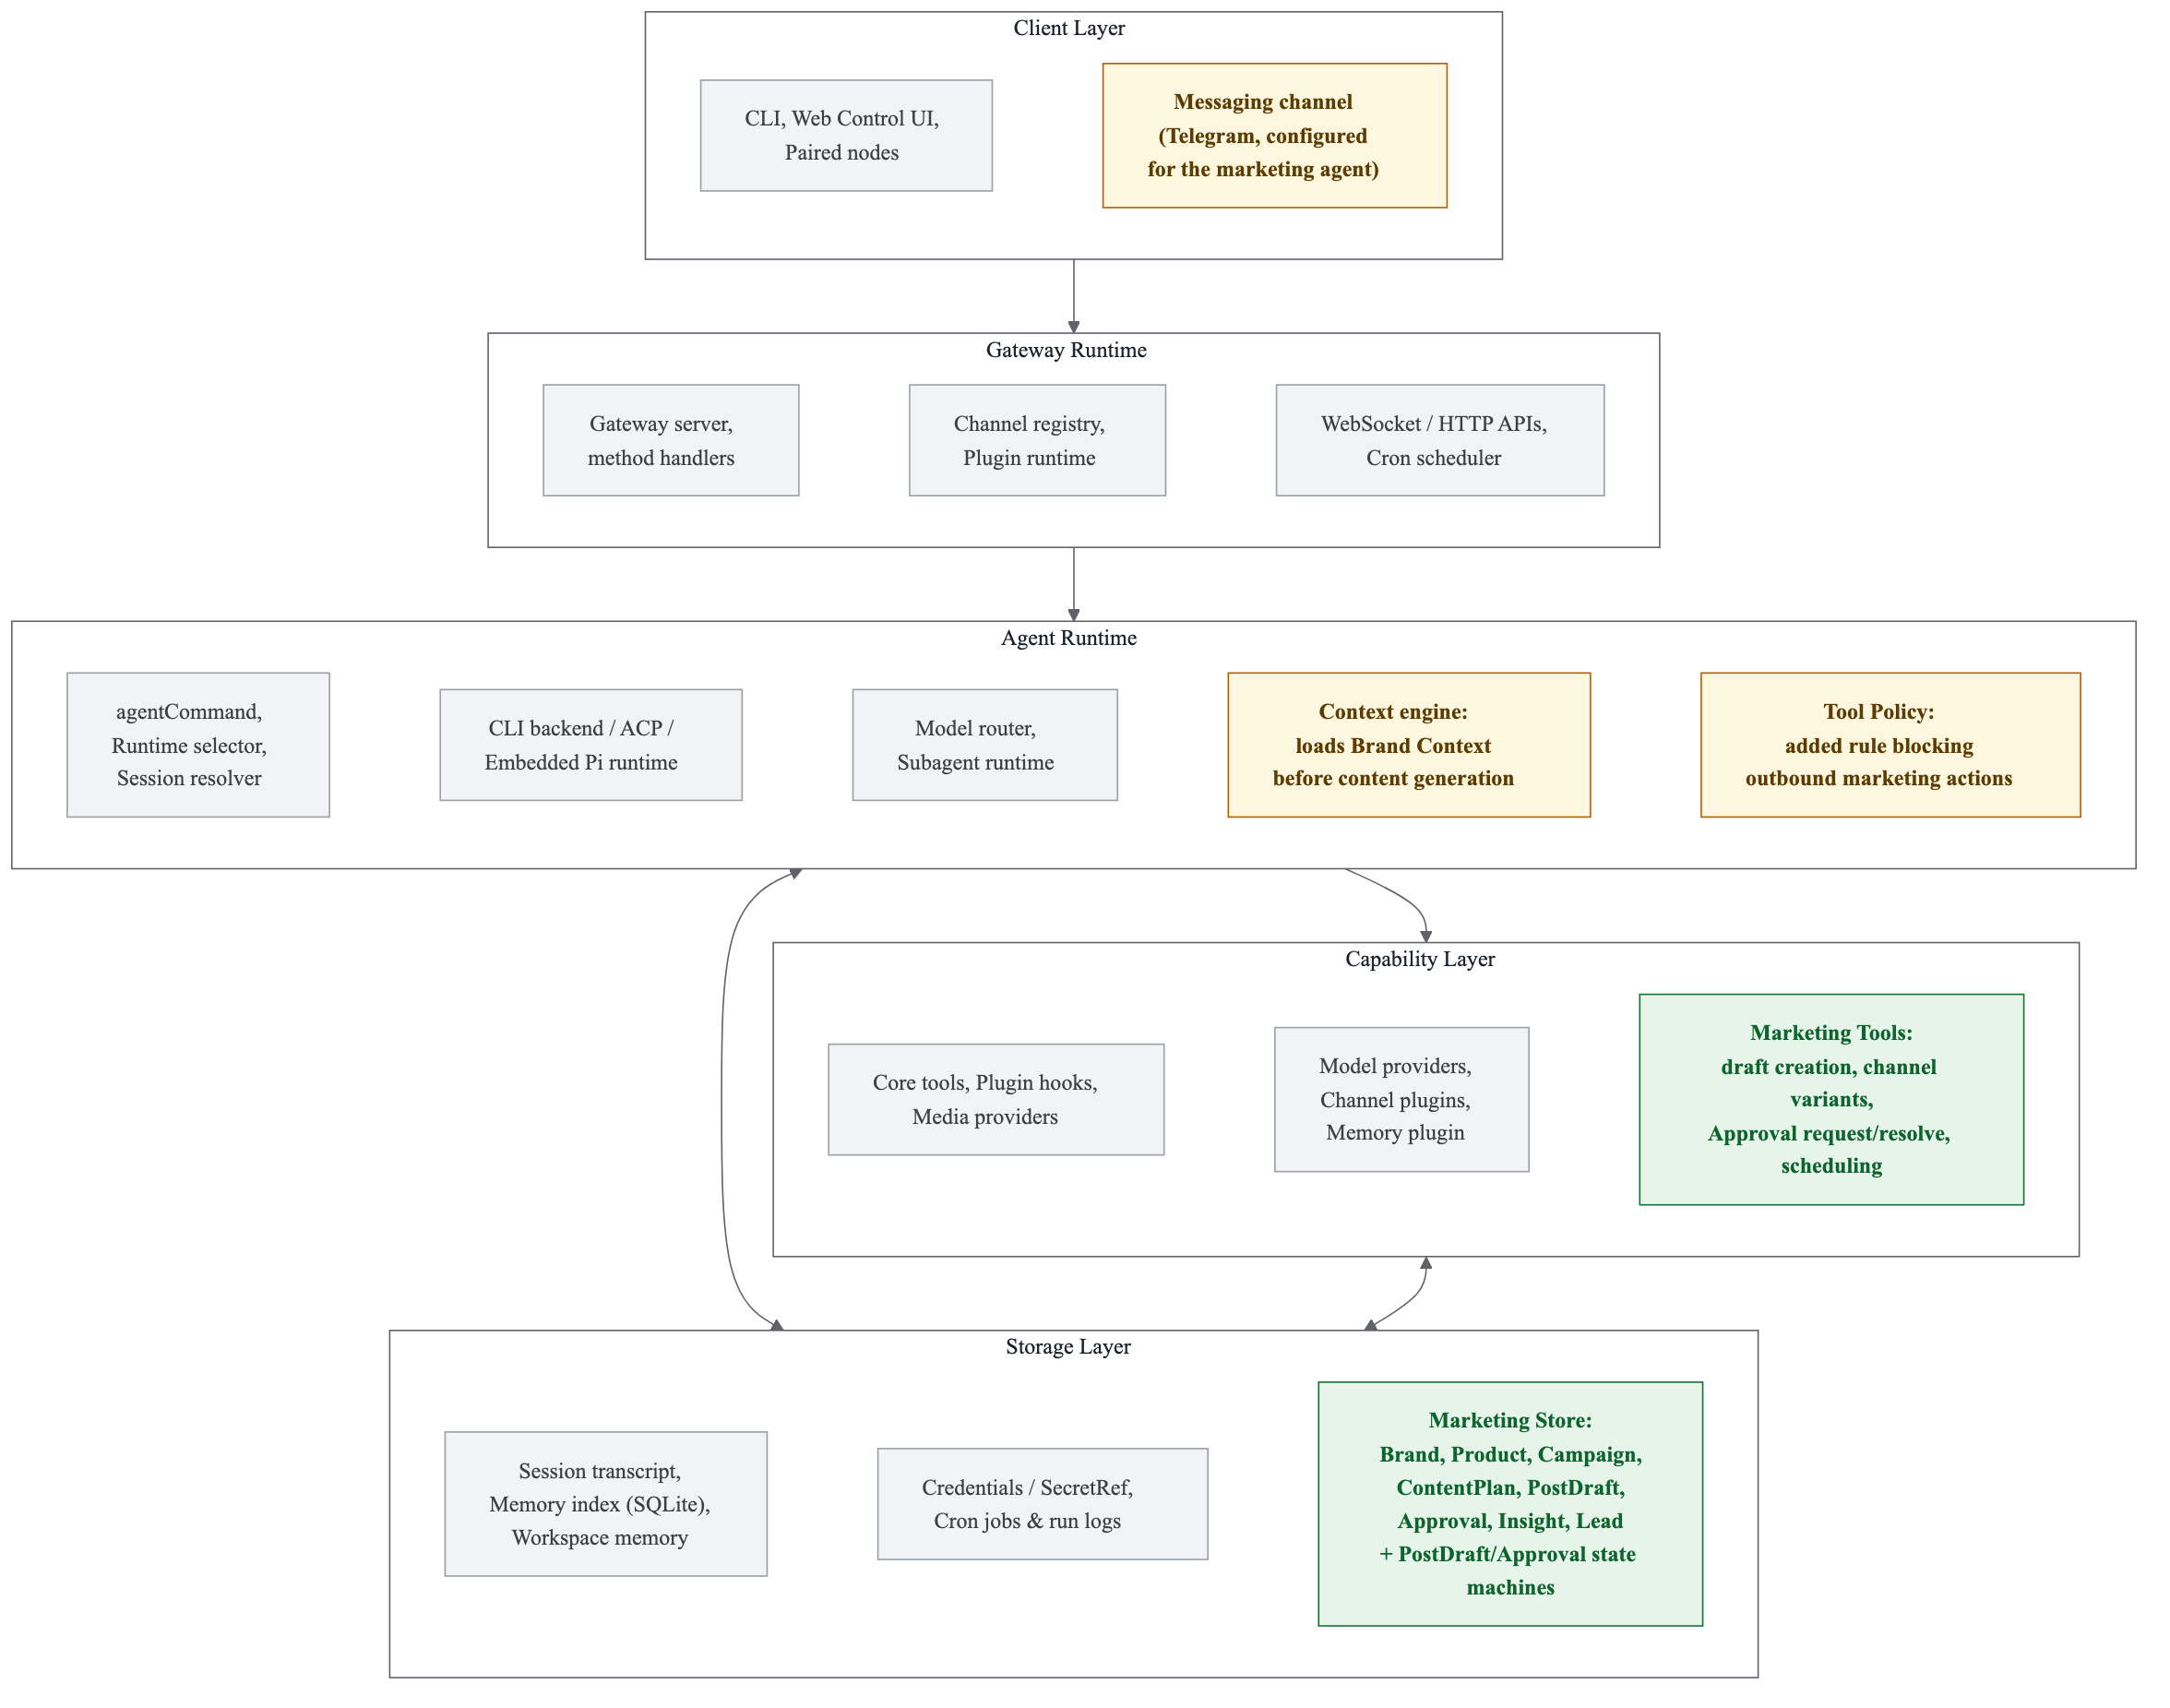
\includegraphics[width=0.95\textwidth,height=0.9\textheight,keepaspectratio]{media/figure_3_1_architecture.png}\caption{Kiến trúc tổng thể của hệ thống, phân biệt phần kế thừa và phần tự xây bằng màu sắc}\end{figure}

Trong Hình 3.1, \textit{Client Layer} là nơi người dùng gửi yêu cầu và nhận kết quả. Lớp này có thể gồm ứng dụng dòng lệnh (\textit{CLI}), giao diện điều khiển web (\textit{Web Control UI}), các nút đã ghép nối (\textit{Paired nodes}) hoặc các ứng dụng nhắn tin đã được cấu hình.

\textit{Gateway Runtime} đóng vai trò trung gian giữa người dùng và \textit{Agent Runtime}. Thành phần này tiếp nhận yêu cầu từ các kênh khác nhau, chuẩn hóa dữ liệu đầu vào và chuyển yêu cầu vào \textit{Agent Runtime} theo một định dạng thống nhất. Nhờ đó, \textit{Agent Runtime} không cần xử lý trực tiếp sự khác nhau giữa từng kênh giao tiếp.

\textit{Agent Runtime} là phần trung tâm của hệ thống. Lớp này nhận yêu cầu đã được chuẩn hóa, xác định Session, nạp các chỉ dẫn hoặc kỹ năng được cấu hình trong Workspace khi có, chuẩn bị ngữ cảnh, chọn đường thực thi, gọi mô hình, kiểm soát công cụ và lưu lại kết quả sau khi hoàn thành lượt xử lý.

\textit{Capability Layer} cung cấp các năng lực mở rộng mà tác nhân có thể sử dụng trong quá trình xử lý. Các năng lực này gồm plugin, công cụ mở rộng, công cụ lõi, kênh giao tiếp, bộ nhớ, thành phần xử lý dữ liệu đa phương tiện và nhà cung cấp mô hình. Nhờ lớp này, hệ thống có thể bổ sung công cụ, kênh giao tiếp, bộ nhớ hoặc nhà cung cấp mô hình mới mà không làm thay đổi cấu trúc xử lý chính.

\textit{Storage Layer} là lớp lưu trữ dữ liệu của hệ thống. Lớp này lưu cấu hình, \textit{Session}, \textit{Transcript}, \textit{Memory}, tác vụ định kỳ, nhật ký vận hành và \textit{SecretRef}. Một số dữ liệu được lưu bằng Markdown, JSON, JSONL hoặc SQLite tùy theo mục đích sử dụng. Nhờ lớp lưu trữ, hệ thống có thể duy trì trạng thái làm việc, truy xuất lại ngữ cảnh và kiểm tra lịch sử xử lý khi cần.

Nhìn tổng thể, hệ thống không xử lý yêu cầu marketing như các câu hỏi rời rạc. Mỗi yêu cầu được đưa qua Gateway Runtime, Agent Runtime, Memory, công cụ và Storage Layer. Cách thiết kế này giúp hệ thống duy trì ngữ cảnh, tái sử dụng thông tin thương hiệu và kiểm soát hành động tốt hơn so với một chatbot chỉ sinh phản hồi theo từng lượt.

Trong Hình 3.1, các khối màu xám thuộc nền tảng tác nhân mã nguồn mở \textit{OpenClaw} có sẵn; hai khối màu vàng (\textit{Context engine}, \textit{Tool Policy}) là phần được điều chỉnh lại cho bài toán marketing; hai khối màu xanh lá (\textit{Marketing Tools}, \textit{Marketing Store}) là phần do đồ án tự xây dựng hoàn toàn mới. Cách tô màu này trả lời trực tiếp câu hỏi ranh giới đóng góp của đồ án. Bảng 3.5 trình bày lại cùng ranh giới này ở mức chi tiết hơn, theo từng thành phần kỹ thuật.

\renewcommand{\arraystretch}{1.25}
\begin{longtable}{L{0.28\textwidth}L{0.42\textwidth}L{0.20\textwidth}}
\caption{Ranh giới giữa nền tảng OpenClaw kế thừa và phần do đồ án điều chỉnh hoặc tự xây dựng}\\
\toprule
\textbf{Thành phần} & \textbf{Vai trò} & \textbf{Kế thừa / Điều chỉnh / Tự xây}\\
\midrule
\endfirsthead
\toprule
\textbf{Thành phần} & \textbf{Vai trò} & \textbf{Kế thừa / Điều chỉnh / Tự xây}\\
\midrule
\endhead

Agent Runtime, Gateway Runtime, Session, Transcript & Vòng lặp xử lý yêu cầu, quản lý phiên làm việc và lưu lịch sử trao đổi. & Kế thừa\\

Memory và memory search (SQLite) & Lưu và truy xuất ngữ cảnh dài hạn theo cơ chế của nền tảng gốc. & Kế thừa\\

Tool Registry, Scheduler, Channel Adapter, Plugin System & Đăng ký công cụ, chạy tác vụ định kỳ và chuẩn hóa dữ liệu kênh giao tiếp. & Kế thừa\\

Context engine (nạp Brand Context trước khi sinh nội dung) & Bổ sung bước lấy thông tin thương hiệu, sản phẩm, khách hàng mục tiêu vào ngữ cảnh trước khi tác nhân suy luận. & Điều chỉnh\\

Tool Policy (rule chặn outbound marketing) & Bổ sung quy tắc chặn đăng bài, gửi hàng loạt hoặc sửa ngân sách khi chưa có Approval hợp lệ. & Điều chỉnh\\

Marketing Tools (tạo bản nháp, biến thể theo kênh, yêu cầu/duyệt Approval, lập lịch bản nháp) & Bộ công cụ marketing được đăng ký vào Tool Registry của nền tảng, không sửa lõi Agent Runtime. & Tự xây\\

Marketing Store (Brand, Product, Campaign, ContentPlan, PostDraft, Approval, Insight, Lead) & Lớp dữ liệu marketing có trạng thái, được lưu ở Storage Layer bên cạnh dữ liệu của nền tảng gốc. & Tự xây\\

Máy trạng thái PostDraft và Approval (Hình 3.11, Hình 3.12) & Định nghĩa vòng đời bản nháp và vòng đời phê duyệt riêng cho hành vi marketing. & Tự xây\\

\bottomrule
\end{longtable}
\renewcommand{\arraystretch}{1}

Nhìn theo bảng trên, phần lõi vận hành của tác nhân (bốn lớp Client, Gateway, phần lớn Agent Runtime và phần lớn Capability/Storage Layer) là kế thừa nguyên trạng từ OpenClaw. Đóng góp của đồ án tập trung ở hai điểm điều chỉnh (nạp Brand Context, mở rộng Tool Policy) và ba khối tự xây mới (Marketing Tools, Marketing Store, hai máy trạng thái PostDraft/Approval). Cách tách này đúng với số liệu kiểm thử đã trình bày ở Bảng 4.4: 247 testcase cho phần nền kế thừa và 61 testcase cho phần marketing tự xây.

So với nền tảng gốc, các thay đổi cụ thể mà đồ án đã thực hiện gồm:

\begin{itemize}
\item Thêm tầng dữ liệu \textit{marketing store} với 8 đối tượng có trạng thái (Brand, Product, Campaign, ContentPlan, PostDraft, Approval, Insight, Lead) — nền tảng gốc không có lớp dữ liệu này.
\item Thêm bộ công cụ marketing (tạo bản nháp, biến thể theo kênh, yêu cầu/duyệt Approval, lập lịch bản nháp) và đăng ký các công cụ này vào Tool Registry sẵn có, không sửa cấu trúc lõi của Agent Runtime.
\item Thêm quy tắc trong Tool Policy để chặn hành động outbound (đăng bài, gửi tin hàng loạt, sửa ngân sách quảng cáo) khi chưa có bản ghi Approval ở trạng thái đã duyệt.
\item Thêm cơ chế nạp Brand Context vào ngữ cảnh trước khi tác nhân sinh nội dung, giúp bản nháp bám đúng giọng văn, khách hàng mục tiêu và ràng buộc thương hiệu đã lưu.
\item Định nghĩa hai máy trạng thái mới: vòng đời bản nháp \textit{PostDraft} (Hình 3.11) và vòng đời yêu cầu phê duyệt \textit{Approval} (Hình 3.12), vốn không tồn tại trong nền tảng gốc.
\end{itemize}

Nói ngắn gọn, nền tảng gốc chỉ dừng ở việc trả lời từng lượt yêu cầu; sau khi bổ sung marketing store và cơ chế phê duyệt, hệ thống giữ được trạng thái của cả chiến dịch qua nhiều lượt làm việc và kiểm soát được hành động nào cần con người xác nhận trước khi thực hiện.

\subsecx{3.3.2. Thiết kế các thành phần chính của tác nhân}

Các thành phần chính của tác nhân được thể hiện trong vùng \textit{Agent Runtime} ở Hình 3.1 và luồng xử lý chi tiết ở Hình 3.2. Đây là nhóm thành phần chịu trách nhiệm điều phối một lượt xử lý của tác nhân, từ lúc nhận yêu cầu đến khi tạo phản hồi và lưu lại kết quả.

Trong một lượt xử lý, hệ thống tiếp nhận yêu cầu từ người dùng và chuẩn hóa yêu cầu đó thành dạng mà \textit{Agent Runtime} có thể xử lý. Sau đó, hệ thống xác định \textit{Session}, lấy các thông tin cần thiết từ \textit{Workspace} và truy xuất ngữ cảnh liên quan để chuẩn bị cho bước gọi mô hình. Tiếp theo, \textit{Runtime selector} chọn môi trường chạy phù hợp, chẳng hạn \textit{CLI backend runtime}, \textit{ACP runtime} hoặc \textit{Embedded Pi agent runtime}.

Sau khi môi trường chạy được chọn, hệ thống xây dựng prompt, chuẩn bị danh sách công cụ được phép sử dụng và gọi mô hình ngôn ngữ lớn thông qua \textit{Model Router}. Nếu mô hình yêu cầu sử dụng công cụ, \textit{Tool Policy} sẽ kiểm tra quyền sử dụng trước khi công cụ được thực thi. Với các yêu cầu phức tạp, hệ thống có thể chia nhỏ nhiệm vụ và điều phối qua \textit{Subagent}.

\begin{figure}[H]\centering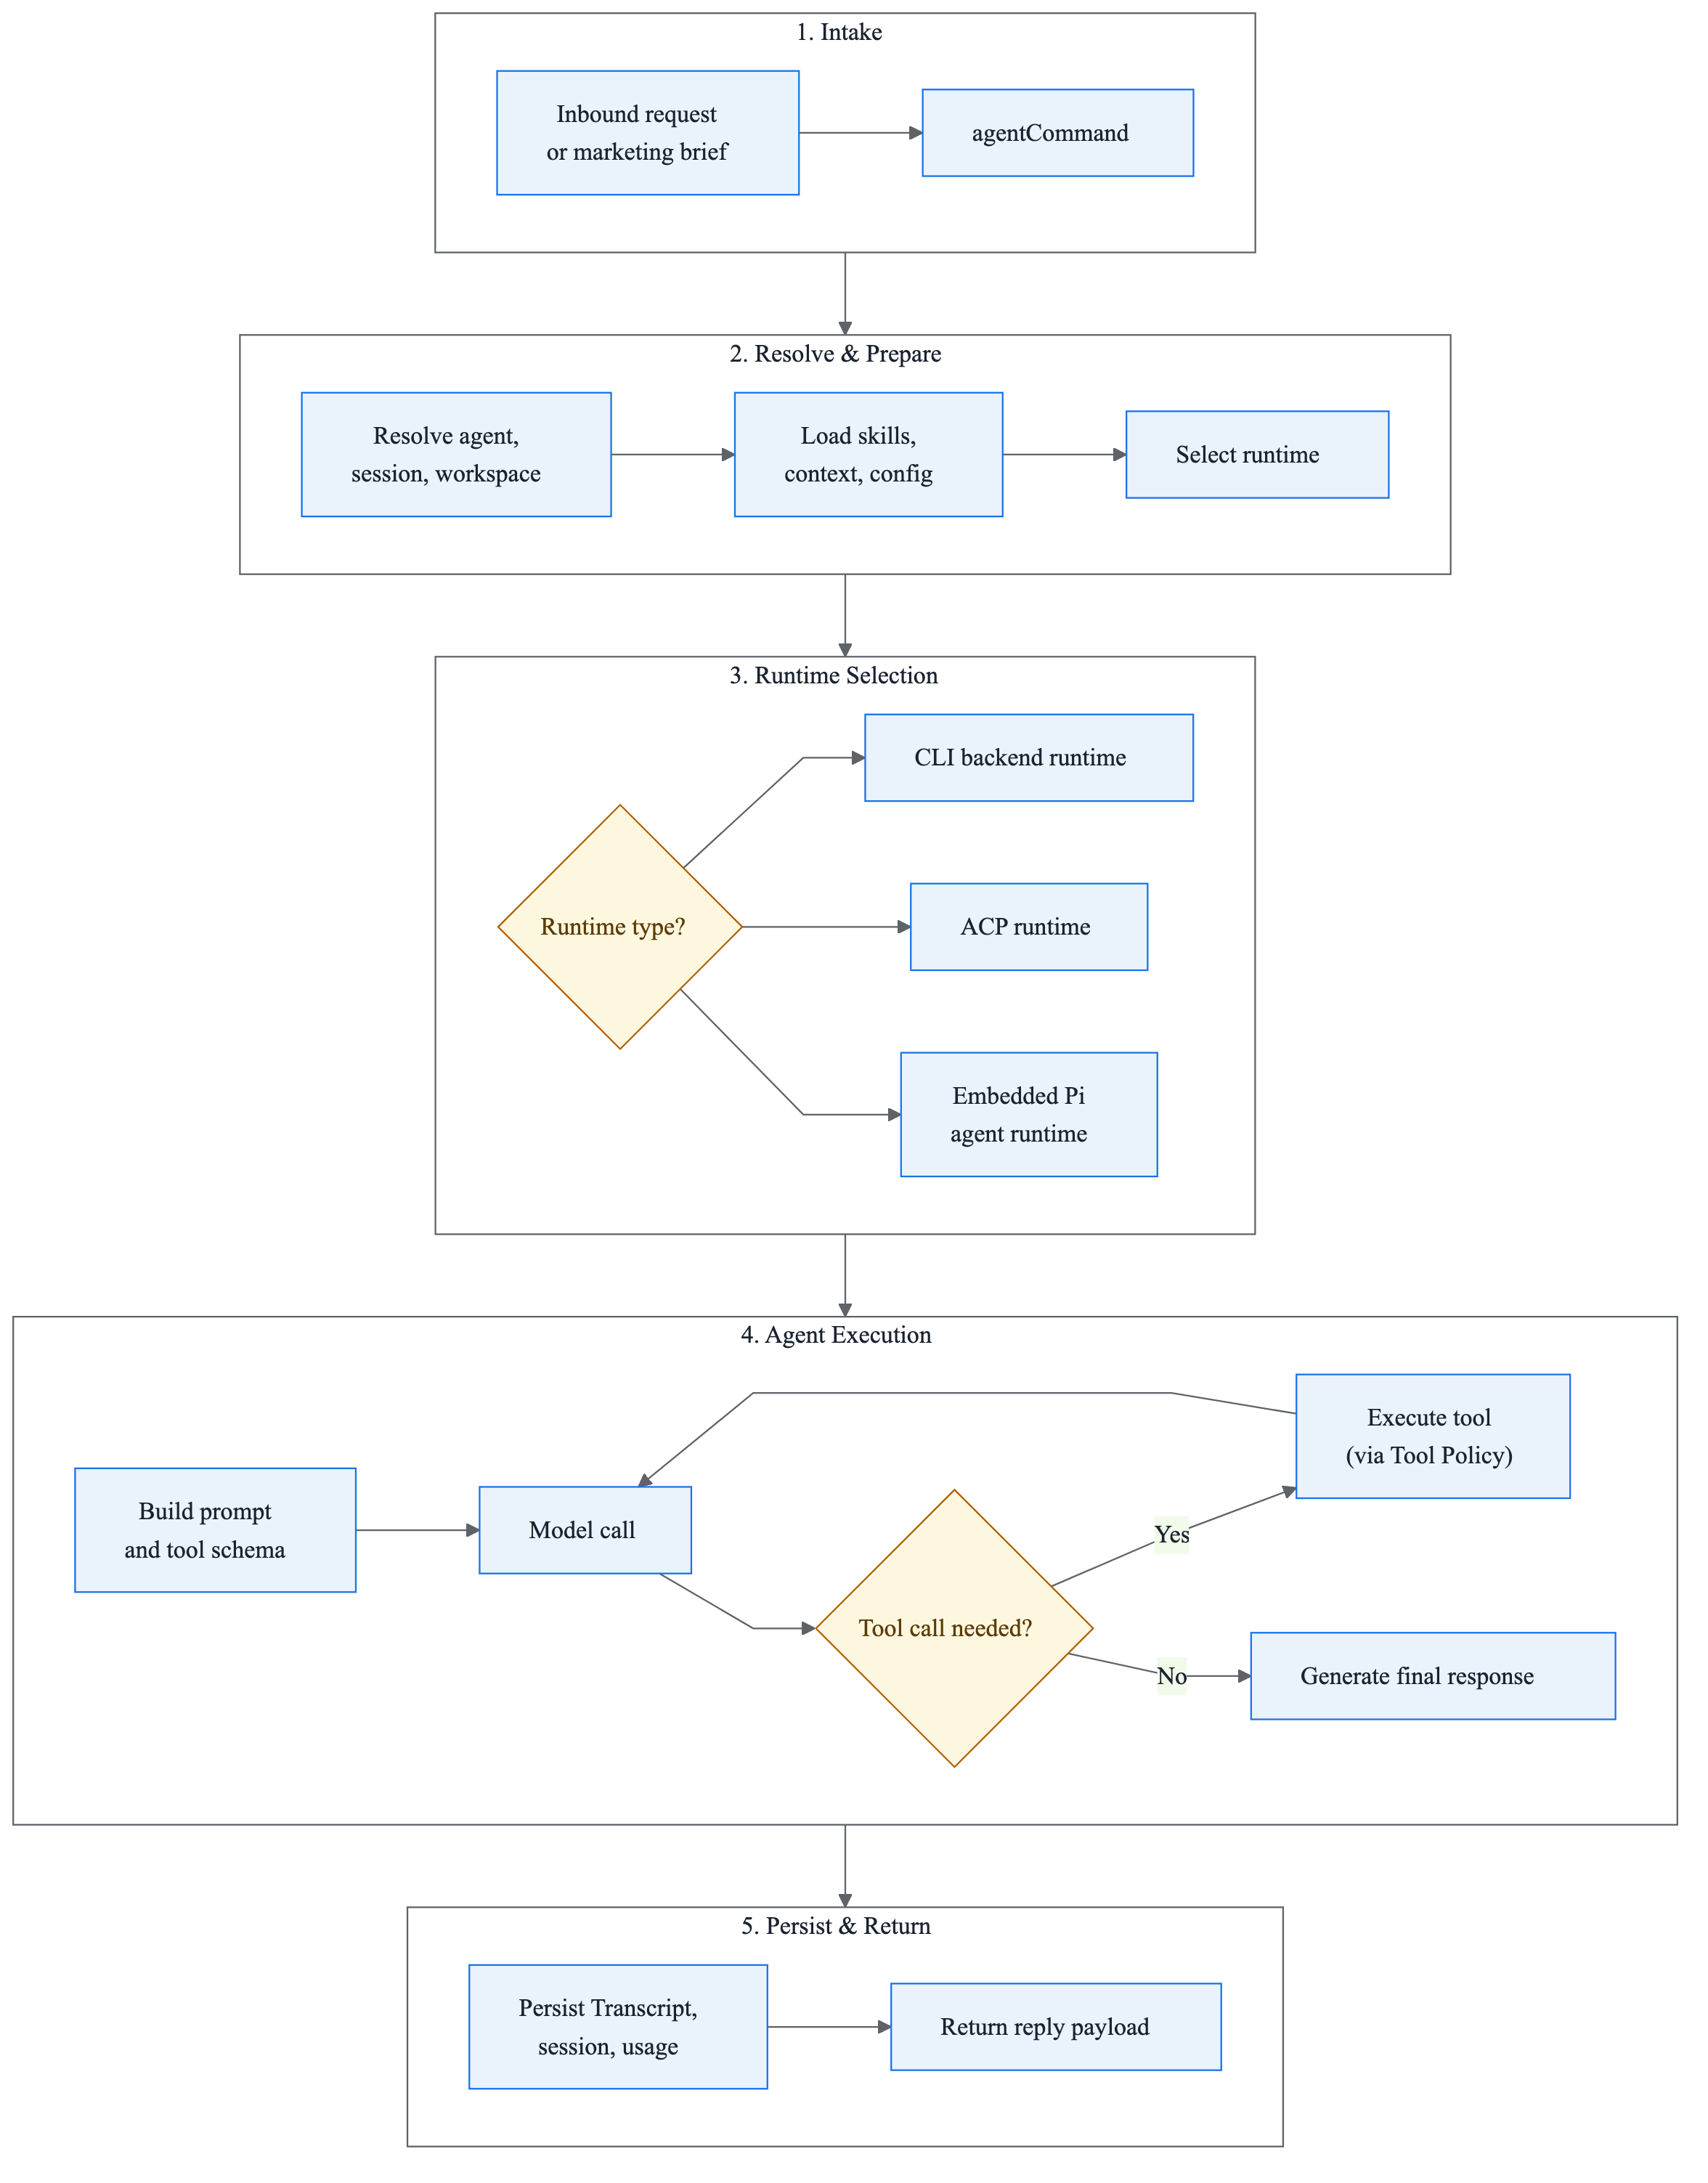
\includegraphics[width=0.9\textwidth,height=0.9\textheight,keepaspectratio]{media/figure_3_2_agent_runtime_flow.png}\caption{Luồng xử lý trong Agent Runtime}\end{figure}

Lệnh tác nhân (\textit{Agent Command}) là điểm bắt đầu của một lượt xử lý trong Agent Runtime. Thành phần này nhận yêu cầu đã chuẩn hóa, kiểm tra thông tin đầu vào và chuyển yêu cầu sang các bước chuẩn bị. Đây là nơi kết nối giữa yêu cầu của người dùng và vòng xử lý bên trong tác nhân.

Bước phân giải và chuẩn bị (\textit{Resolve \& Prepare}) xác định tác nhân cần dùng, Session, Workspace, cấu hình, kỹ năng trong Workspace khi có và ngữ cảnh liên quan. Bước này quan trọng vì yêu cầu marketing thường phụ thuộc vào thương hiệu, sản phẩm, khách hàng mục tiêu và lịch sử làm việc trước đó.

Bộ chọn đường chạy (\textit{Runtime selector}) quyết định yêu cầu sẽ được xử lý bằng đường chạy nào. Theo sơ đồ, hệ thống có ba đường chính: chạy qua dòng lệnh, chạy qua ACP hoặc chạy qua Embedded Pi agent runtime. Trong phạm vi đồ án, nội dung cần nhấn mạnh là Agent Runtime không bị khóa vào một cách chạy duy nhất; hệ thống có thể chọn đường chạy phù hợp với cấu hình và môi trường.

Ở bước thực thi tác nhân (\textit{Agent Execution}), hệ thống xây dựng prompt và cấu trúc mô tả các công cụ được phép dùng, gọi mô hình, kiểm tra mô hình có yêu cầu gọi công cụ hay không, thực thi công cụ nếu được phép, rồi trả kết quả cuối cùng. Kết quả sau đó được chuyển sang bước lưu và trả phản hồi.

\textit{Tool Registry} quản lý các công cụ mà tác nhân có thể dùng. Mỗi công cụ có tên, mô tả, cấu trúc tham số và hàm thực thi. \textit{Tool Policy} quyết định công cụ nào được phép dùng trong từng lượt chạy. Mô hình ngôn ngữ chỉ đề xuất lời gọi công cụ; hệ thống vẫn phải kiểm tra công cụ, tham số và quyền trước khi thực thi.

\imgfig{media/image4.png}{Quy trình đăng ký, kiểm soát và thực thi công cụ}

Hình 3.3 cho thấy công cụ có thể đến từ hai nguồn: công cụ lõi của hệ thống và công cụ do plugin cung cấp. Sau khi được đăng ký vào Tool Registry, danh sách công cụ đi qua Tool Policy. Chỉ các công cụ hợp lệ mới được chuyển thành cấu trúc mô tả công cụ cho mô hình. Khi mô hình trả về yêu cầu gọi công cụ, hệ thống thực thi công cụ rồi đưa kết quả về lại mô hình để tiếp tục xử lý.

Plugin System là cách mở rộng chức năng của hệ thống. Plugin có thể bổ sung công cụ mới, Model Provider, kênh giao tiếp hoặc thành phần Memory. Tuy nhiên, plugin không được vượt qua Tool Policy. Mọi năng lực bổ sung vẫn phải đi qua cơ chế đăng ký và lọc công cụ để giảm rủi ro khi đọc, ghi hoặc gửi dữ liệu.

\imgfig{media/imagea.png}{Luồng nạp plugin và đăng ký năng lực mở rộng}

\textit{Model Provider} là thành phần kết nối đến mô hình ngôn ngữ lớn. \textit{Model Router} chọn Model Provider và mô hình theo cấu hình, điểm móc mở rộng hoặc cơ chế dự phòng. Trong đồ án, thành phần này không nhằm so sánh chất lượng giữa các mô hình, mà nhằm tách cấu hình mô hình khỏi Agent Runtime để hệ thống dễ thay đổi và bảo trì.

\imgfig{media/imageb.png}{Luồng chọn Model Provider và thực thi mô hình}

\textit{Subagent Runtime} hỗ trợ chia một yêu cầu lớn thành các phần nhỏ hơn. Ví dụ, một yêu cầu lập kế hoạch chiến dịch có thể được chia thành phân tích khách hàng, đề xuất hướng nội dung, viết bản nháp và tổng hợp kết quả. Trong phạm vi đồ án, Subagent Runtime là năng lực kỹ thuật hỗ trợ xử lý tác vụ phức tạp, không phải một vai trò marketing độc lập đã được hiện thực đầy đủ.

\imgfig{media/imagec.png}{Luồng điều phối Subagent Runtime}

Tóm lại, Agent Runtime không chỉ gọi mô hình để sinh văn bản. Nó còn phân giải Session, nạp ngữ cảnh, chọn mô hình, lắp danh sách công cụ được phép dùng, xử lý lượt gọi công cụ và lưu kết quả. Đây là phần làm cho hệ thống có trạng thái và có khả năng vận hành theo quy trình thay vì chỉ trả lời từng câu hỏi đơn lẻ.

\subsecx{3.3.3. Thiết kế Memory, Session và lưu trữ dữ liệu}

Memory, Workspace và Session giúp hệ thống xử lý yêu cầu có ngữ cảnh. Đây là điểm khác biệt quan trọng giữa hệ thống tác nhân và chatbot thông thường. Nếu không có các thành phần này, mỗi lần tạo nội dung hoặc lập kế hoạch mới đều phải nhập lại thông tin thương hiệu, sản phẩm, giọng văn và các ràng buộc đã thống nhất trước đó.

\textit{Workspace} chứa cấu hình, các tệp liên quan đến quá trình vận hành hệ thống. Memory dài hạn lưu các thông tin có thể dùng lại như thông tin thương hiệu, sản phẩm, khách hàng mục tiêu, giọng văn, nội dung đã được duyệt hoặc nhận xét quan trọng. Khi xử lý yêu cầu mới, hệ thống có thể truy xuất các thông tin liên quan để đưa vào ngữ cảnh.

\imgfig{media/image5.png}{Luồng Memory, Workspace và truy xuất ngữ cảnh}

\textit{Session} dùng để tách biệt các luồng trao đổi. Một Session có thể gắn với người dùng, kênh giao tiếp, hội thoại nhóm, tác vụ định kỳ hoặc tác nhân con. Ví dụ, Session lập kế hoạch nội dung không nên bị trộn với Session tạo báo cáo quảng cáo. Việc tách Session giúp Transcript và ngữ cảnh được lưu đúng phạm vi.

\imgfig{media/image6.png}{Luồng phân giải Session và lưu Transcript}

\textit{Transcript} lưu lại các lượt tương tác, lời gọi công cụ và kết quả công cụ theo thứ tự thời gian. Memory dài hạn không thay thế Transcript. Transcript dùng để xem lại diễn biến của một Session, còn Memory dài hạn dùng để lưu các thông tin có giá trị sử dụng lại trong nhiều Session.

\imgfig{media/imaged.png}{Luồng lưu Transcript và các thành phần sử dụng}

Dữ liệu của hệ thống được lưu theo từng nhóm để phù hợp với mục đích sử dụng. Các thông tin cần đọc và chỉnh sửa thủ công, như ghi nhớ dài hạn hoặc thông tin thương hiệu, được lưu bằng Markdown. Cấu hình hệ thống được lưu bằng JSON hoặc JSON5. Lịch sử trao đổi, lượt gọi công cụ và nhật ký chạy tác vụ được lưu bằng JSONL để thuận tiện cho việc ghi nối tiếp theo thời gian. SQLite được dùng để tạo chỉ mục tìm kiếm cho \textit{Memory}.

Cách tổ chức này giúp hệ thống vừa lưu được lịch sử xử lý, vừa truy xuất được thông tin cần thiết khi xử lý yêu cầu mới. Khi gọi mô hình ngôn ngữ lớn, hệ thống chỉ chọn những phần dữ liệu liên quan để đưa vào ngữ cảnh, thay vì đưa toàn bộ dữ liệu đã lưu.

\renewcommand{\arraystretch}{1.25}
\begin{longtable}{L{0.25\textwidth}L{0.20\textwidth}L{0.45\textwidth}}
\caption{Dữ liệu lưu trữ chính của hệ thống}\\
\toprule
\textbf{Nhóm dữ liệu} & \textbf{Định dạng} & \textbf{Vai trò}\\
\midrule
\endfirsthead
\toprule
\textbf{Nhóm dữ liệu} & \textbf{Định dạng} & \textbf{Vai trò}\\
\midrule
\endhead

Cấu hình hệ thống & JSON/JSON5 & Lưu thông tin Model Provider, công cụ, kênh giao tiếp, đường dẫn Workspace và Tool Policy mặc định.\\

Thông tin Session & JSON & Lưu trạng thái Session, kênh giao tiếp, người dùng, mô hình và thời điểm cập nhật.\\

Transcript & JSONL & Lưu từng lượt tương tác, lời gọi công cụ và kết quả trả về theo thứ tự thời gian.\\

Memory dài hạn & Markdown & Lưu thông tin thương hiệu, quyết định, nhận xét và quy tắc vận hành.\\

Chỉ mục Memory & SQLite & Hỗ trợ tìm kiếm thông tin trong Memory theo nội dung liên quan.\\

Tác vụ định kỳ & JSON & Lưu lịch chạy, trạng thái, chủ sở hữu và tham số của tác vụ định kỳ.\\

Nhật ký chạy tác vụ & JSONL & Lưu lịch sử chạy tác vụ định kỳ, kết quả thực thi và lỗi nếu có.\\

SecretRef & Tham chiếu & Lưu tham chiếu đến thông tin xác thực, không đưa khóa bí mật trực tiếp vào prompt hoặc Transcript.\\

\bottomrule
\end{longtable}
\renewcommand{\arraystretch}{1}

\subsecx{3.3.4. Thiết kế mô hình dữ liệu marketing store}

Như đã trình bày ở mục trước, điểm khác biệt quan trọng giữa hệ thống tác nhân và chatbot thông thường là thông tin không chỉ tồn tại trong nội dung hội thoại mà được lưu thành dữ liệu có cấu trúc. Để hỗ trợ công việc marketing diễn ra qua nhiều bước và nhiều lượt làm việc, hệ thống cần một nơi lưu trữ riêng cho các đối tượng marketing, gọi là \textit{marketing store}. Nhờ lớp dữ liệu này, tác nhân có thể ghi nhớ thông tin thương hiệu, sản phẩm, chiến dịch và các bản nháp đã tạo, sau đó truy xuất lại trong các bước xử lý tiếp theo thay vì yêu cầu người dùng nhập lại từ đầu.

Hình 3.10 mô tả các đối tượng dữ liệu chính trong marketing store và mối quan hệ giữa chúng. Mô hình được tổ chức xoay quanh thương hiệu và chiến dịch, từ đó dẫn tới kế hoạch nội dung, bản nháp bài đăng và cơ chế phê duyệt.

\begin{figure}[H]\centering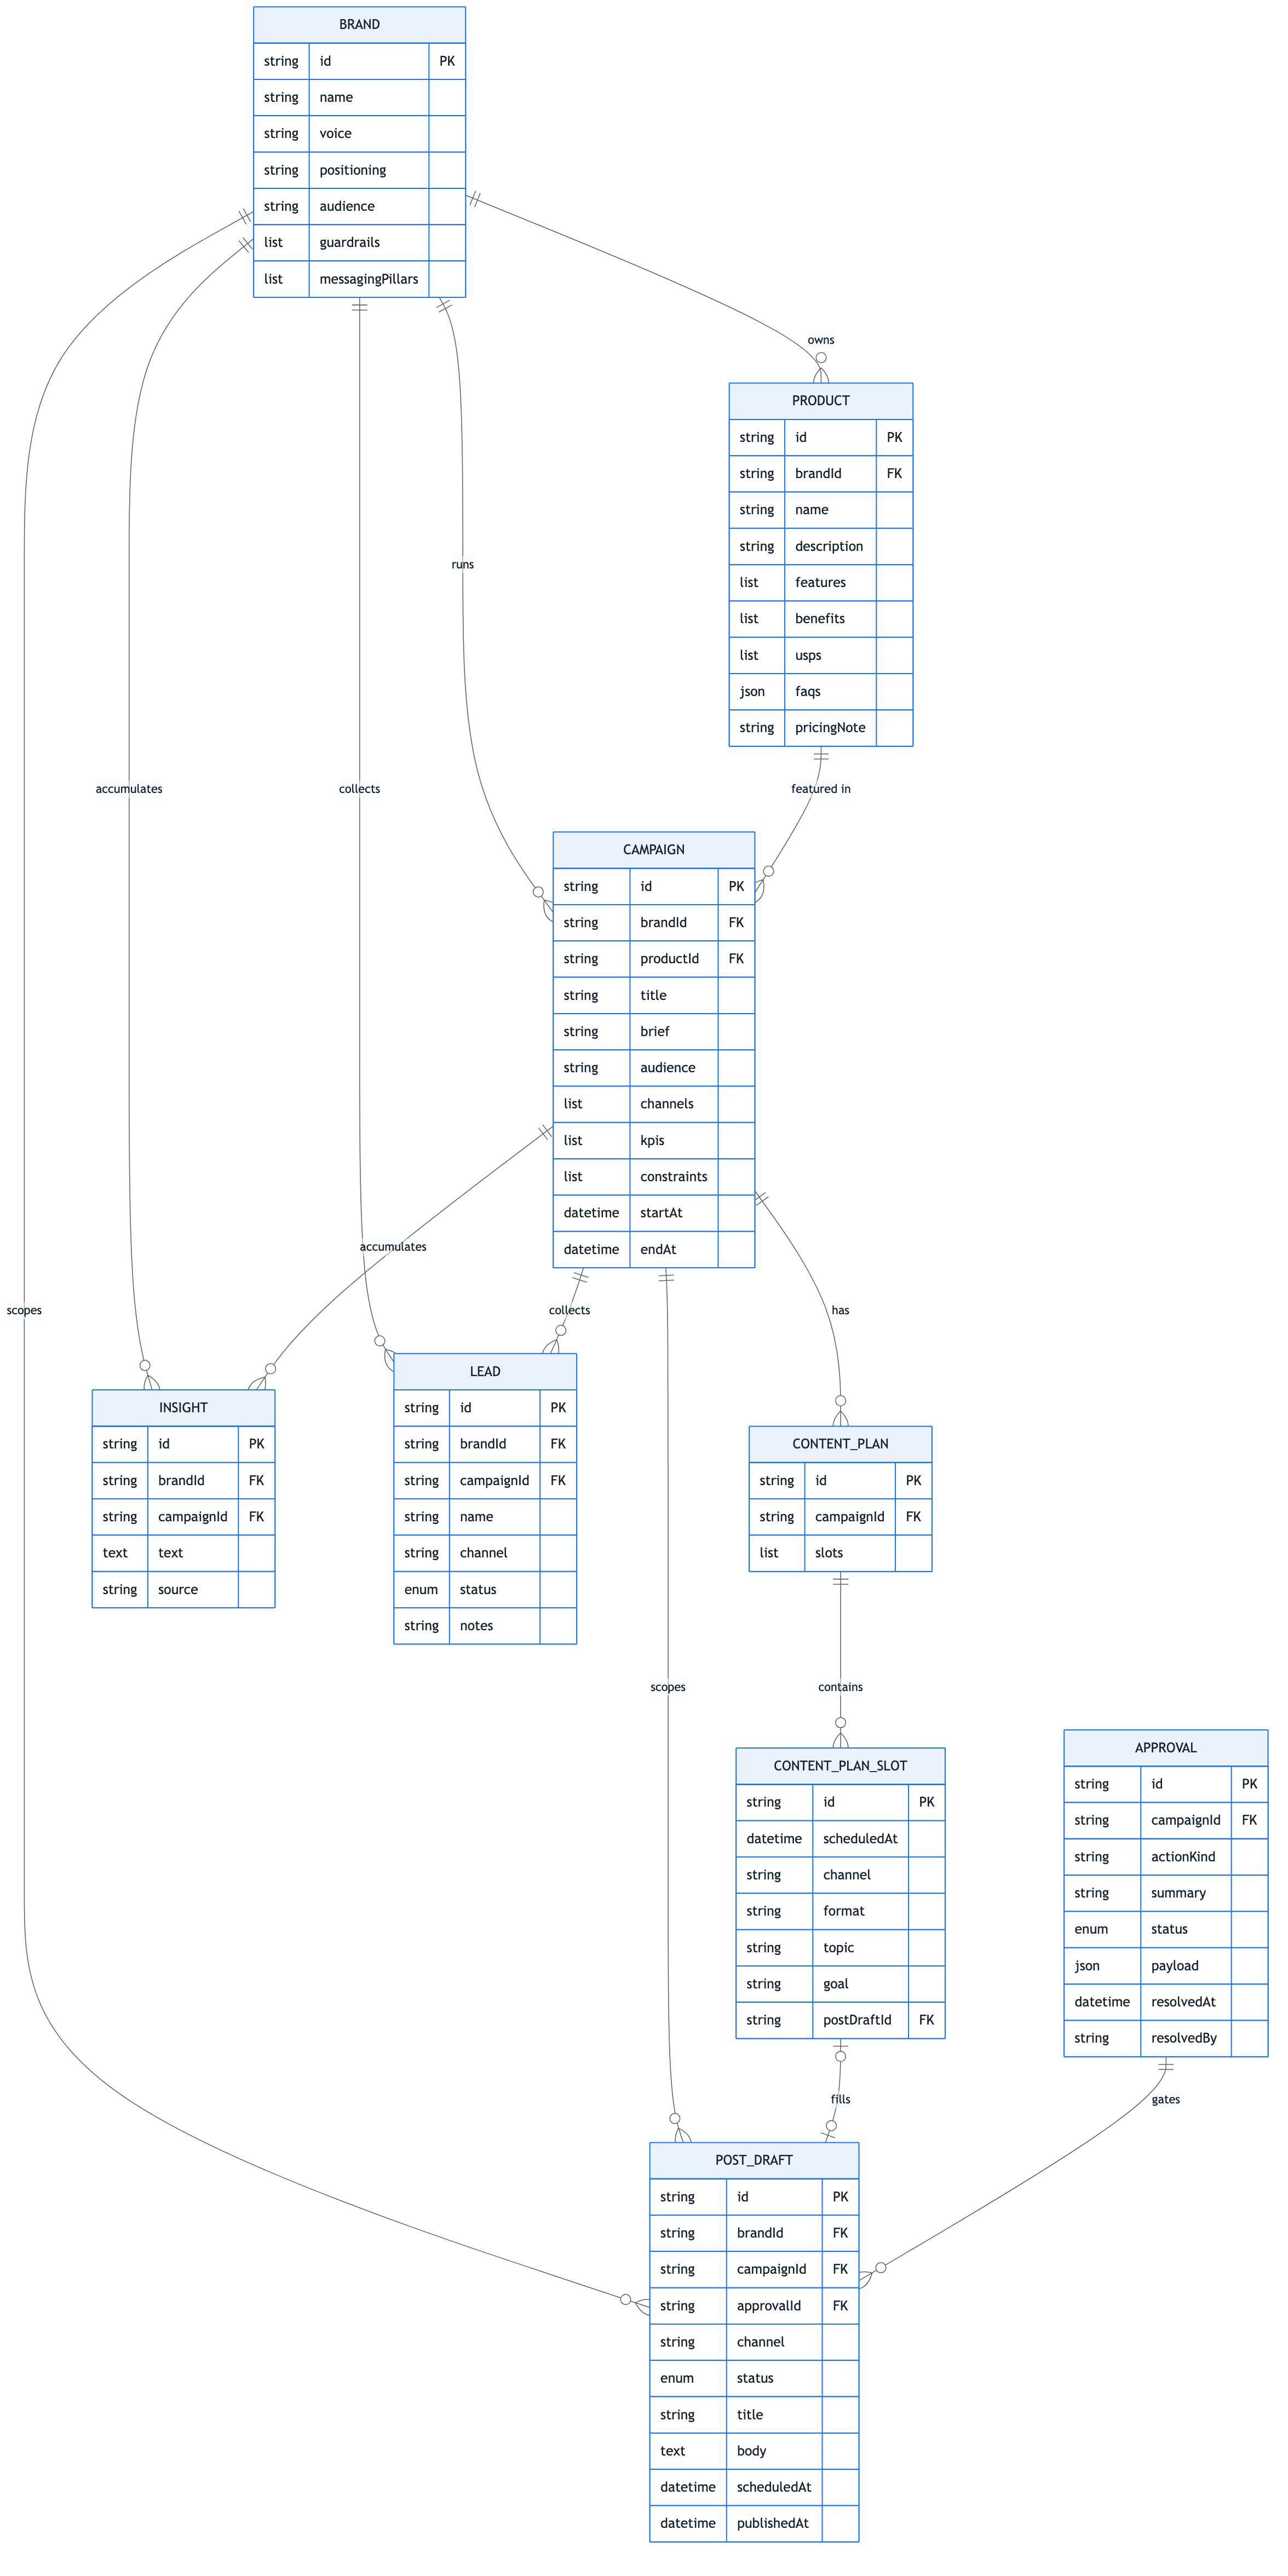
\includegraphics[width=0.92\textwidth,height=0.86\textheight,keepaspectratio]{media/figure_3_10_marketing_store_erd.png}\caption{Mô hình dữ liệu các đối tượng chính trong marketing store}\end{figure}

Có thể chia các đối tượng trong Hình 3.10 thành bốn nhóm theo vai trò:

\begin{itemize}
\item \textbf{Nhóm nền tảng thương hiệu và sản phẩm.} \textit{Brand} lưu thông tin thương hiệu như giọng văn, định vị, khách hàng mục tiêu, trụ cột thông điệp và các ràng buộc nội dung. \textit{Product} lưu thông tin sản phẩm như mô tả, tính năng, lợi ích, điểm bán hàng độc nhất và câu hỏi thường gặp. Mỗi sản phẩm gắn với một thương hiệu.
\item \textbf{Nhóm kế hoạch và nội dung.} \textit{Campaign} mô tả một chiến dịch với tóm tắt yêu cầu, kênh dự kiến, chỉ số đo lường, ràng buộc và mốc thời gian. \textit{ContentPlan} là kế hoạch nội dung của chiến dịch, gồm nhiều khung nội dung (\textit{ContentPlanSlot}) ứng với thời điểm, kênh, định dạng và mục tiêu cụ thể. Mỗi khung nội dung có thể được hiện thực thành một \textit{PostDraft}, là bản nháp bài đăng cho một kênh nhất định.
\item \textbf{Nhóm kiểm soát phê duyệt.} \textit{Approval} ghi nhận yêu cầu phê duyệt cho các hành động nhạy cảm như đăng bài, gửi tin hàng loạt hoặc thao tác với quảng cáo. Một bản ghi phê duyệt có thể gắn với một hoặc nhiều bản nháp khi cùng một nội dung được phát hành trên nhiều kênh.
\item \textbf{Nhóm học hỏi và khách hàng tiềm năng.} \textit{Insight} lưu các nhận xét và bài học rút ra để dùng lại về sau. \textit{Lead} lưu thông tin khách hàng tiềm năng cùng trạng thái theo dõi. Cả hai đều có thể gắn với thương hiệu và chiến dịch tương ứng.
\end{itemize}

Các đối tượng được liên kết với nhau bằng khóa tham chiếu thay vì lồng toàn bộ dữ liệu vào nhau. Ví dụ, một chiến dịch tham chiếu tới thương hiệu và sản phẩm; một kế hoạch nội dung tham chiếu tới chiến dịch; một bản nháp tham chiếu tới thương hiệu, chiến dịch và bản ghi phê duyệt liên quan. Cách tổ chức này giúp dữ liệu nhất quán, dễ truy xuất và tránh trùng lặp khi cùng một thương hiệu hoặc sản phẩm được dùng cho nhiều chiến dịch.

Trọng tâm của lớp dữ liệu này là đối tượng \textit{PostDraft}, vì hầu hết quy trình tạo và phát hành nội dung đều xoay quanh vòng đời của bản nháp. Hình 3.11 mô tả các trạng thái mà một bản nháp đi qua, từ ý tưởng ban đầu cho tới khi được đo lường kết quả.

\begin{figure}[H]\centering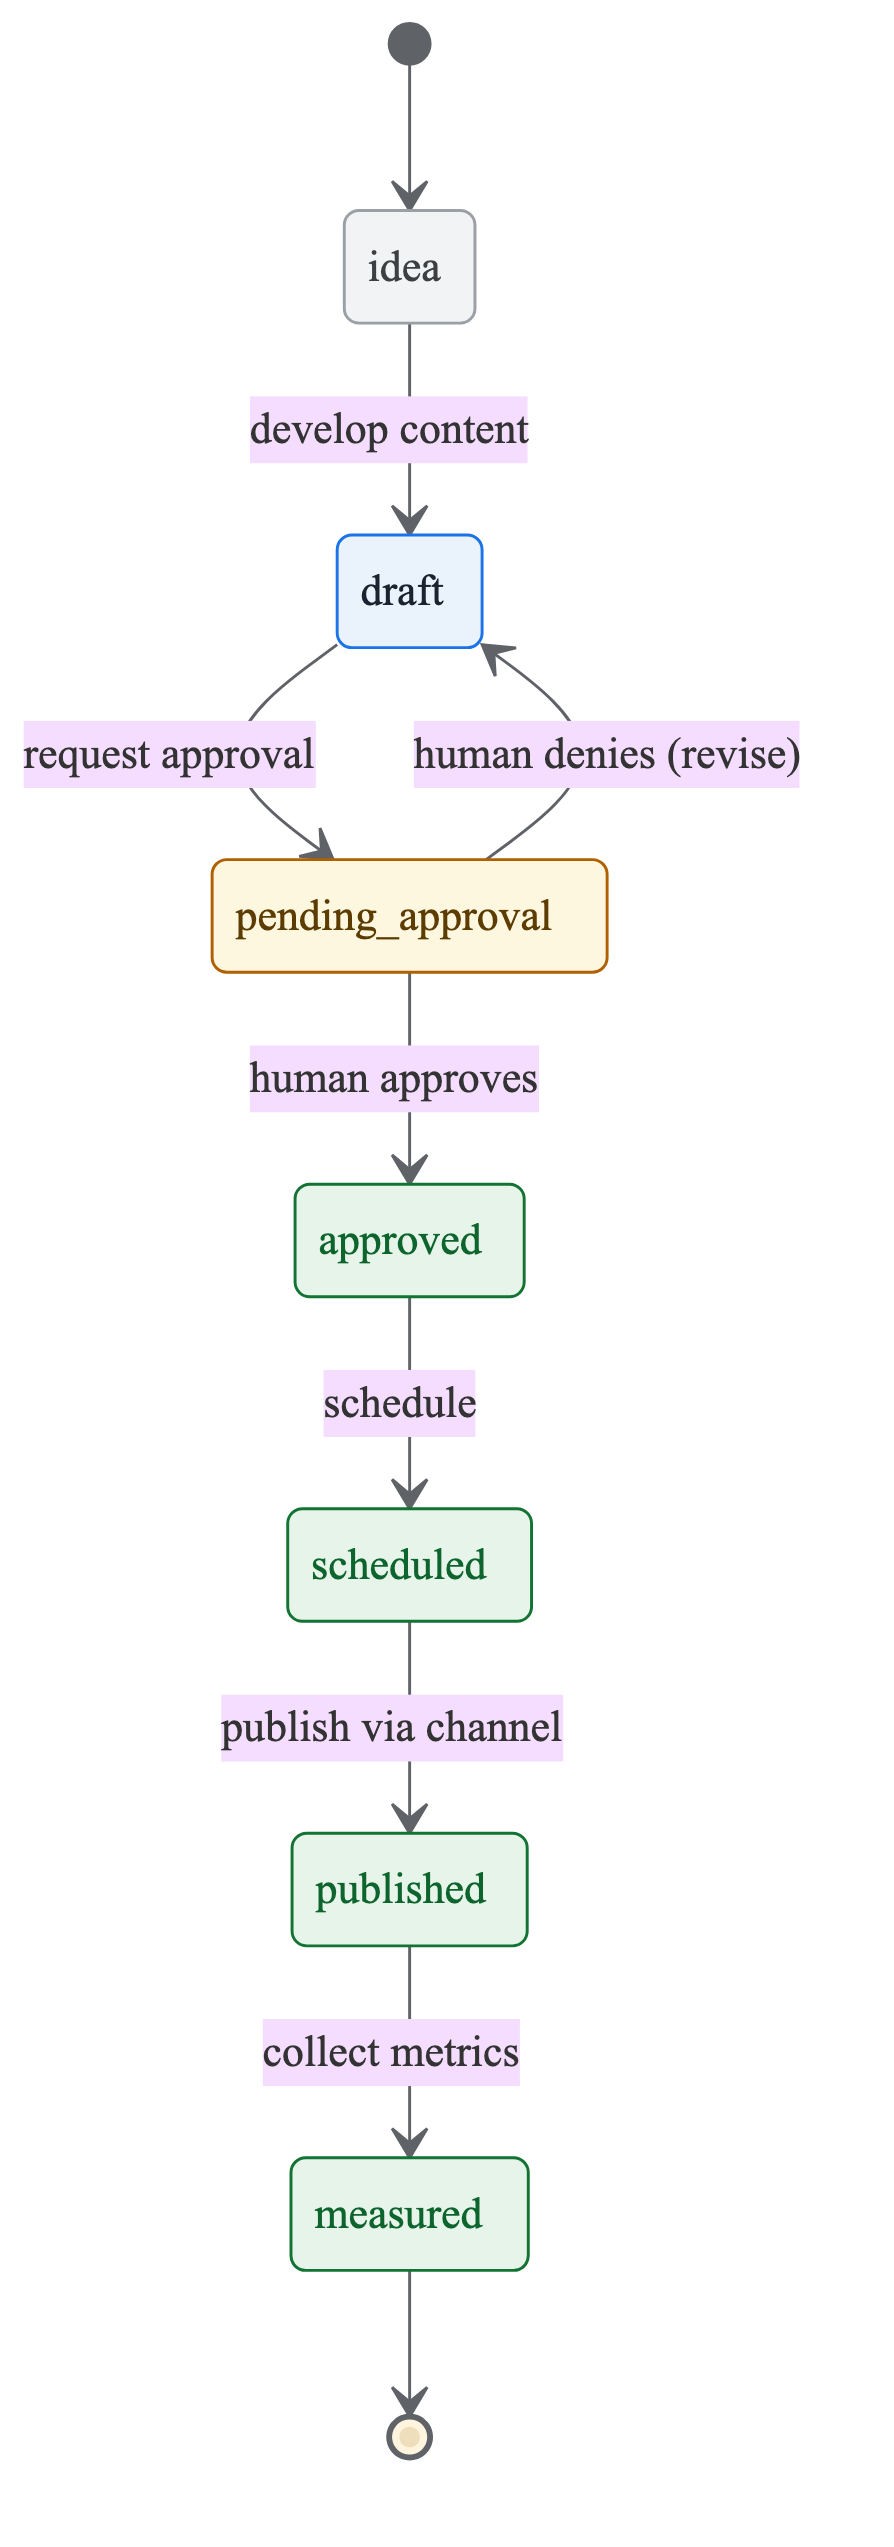
\includegraphics[width=0.9\textwidth,height=0.85\textheight,keepaspectratio]{media/figure_3_11_postdraft_lifecycle.png}\caption{Vòng đời của một bản nháp bài đăng (PostDraft)}\end{figure}

Bản nháp bắt đầu ở trạng thái ý tưởng (\textit{idea}), sau đó được phát triển thành bản nháp hoàn chỉnh (\textit{draft}). Khi cần phát hành, bản nháp chuyển sang trạng thái chờ phê duyệt (\textit{pending\_approval}). Nếu người phụ trách đồng ý, bản nháp chuyển sang trạng thái đã duyệt (\textit{approved}), rồi được lên lịch (\textit{scheduled}) và phát hành qua kênh (\textit{published}); nếu bị từ chối, bản nháp quay lại để chỉnh sửa. Sau khi phát hành, bản nháp có thể chuyển sang trạng thái đã đo lường (\textit{measured}) để ghi nhận kết quả. Điểm quan trọng là bản nháp không thể tự chuyển sang trạng thái phát hành nếu chưa đi qua bước phê duyệt của con người.

Cơ chế phê duyệt được mô hình hóa bằng đối tượng \textit{Approval} với vòng đời riêng, thể hiện ở Hình 3.12. Mỗi khi tác nhân chuẩn bị thực hiện một hành động nhạy cảm, hệ thống tạo một yêu cầu phê duyệt ở trạng thái chờ (\textit{pending}). Người dùng có thể đồng ý (\textit{approved}), từ chối (\textit{denied}) hoặc để yêu cầu hết hạn (\textit{expired}). Chỉ khi yêu cầu được đồng ý thì hành động tương ứng mới được phép thực hiện; các trường hợp còn lại đều dẫn đến việc chặn hành động.

\begin{figure}[H]\centering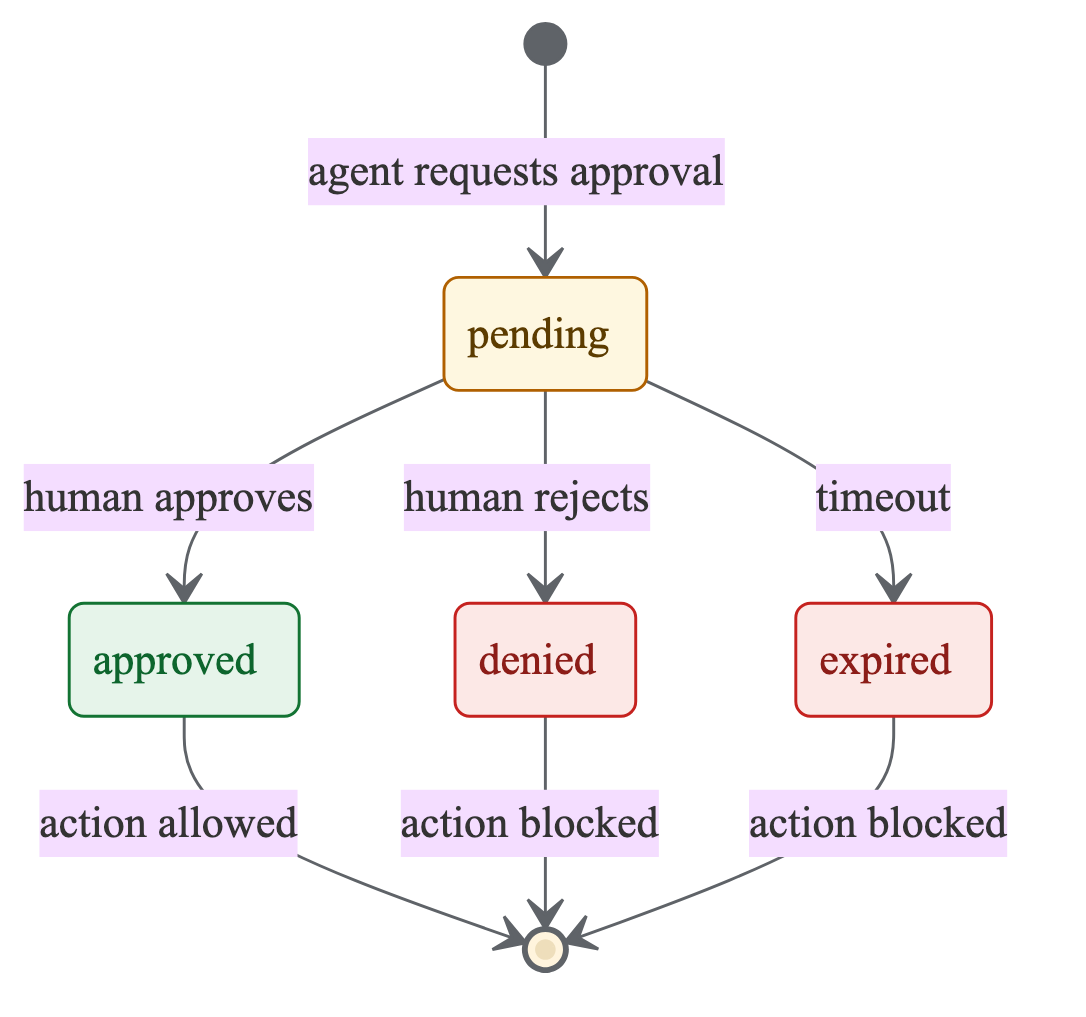
\includegraphics[width=0.85\textwidth,height=0.6\textheight,keepaspectratio]{media/figure_3_12_approval_lifecycle.png}\caption{Vòng đời của một yêu cầu phê duyệt (Approval)}\end{figure}

Hai vòng đời ở Hình 3.11 và Hình 3.12 cùng hiện thực nguyên tắc đọc trước, tạo bản nháp trước, phê duyệt trước khi ghi ra bên ngoài. Nguyên tắc này được trình bày chi tiết hơn ở mục 3.3.7, và là cơ sở để hệ thống giữ vai trò hỗ trợ tạo bản nháp và điều phối, thay vì tự ý thực hiện các hành động có rủi ro ra bên ngoài.

\subsecx{3.3.5. Thiết kế kênh tương tác và phối hợp nhóm}

Trong phạm vi đồ án, hệ thống không tập trung xây dựng giao diện đồ họa hoàn chỉnh. Kênh tương tác được hiểu là cách người dùng gửi yêu cầu và nhận kết quả từ tác nhân. Các kênh này có thể là giao diện dòng lệnh, giao diện web nội bộ hoặc kênh giao tiếp đã cấu hình.

\imgfig{media/figure_3_13_channel_flow.png}{Luồng giao tiếp qua kênh cấu hình của hệ thống}

Channel Adapter chuẩn hóa dữ liệu giữa từng kênh cụ thể và định dạng chung của hệ thống. Nhờ đó, Agent Runtime không cần hiểu chi tiết kỹ thuật của từng kênh. Ví dụ, dữ liệu từ dòng lệnh, web hoặc kênh nhắn tin đều được chuyển thành yêu cầu có cấu trúc trước khi đi vào Agent Runtime.

Thiết kế này cũng hỗ trợ phối hợp nhóm ở mức nền tảng. Một thành viên có thể yêu cầu tạo bản nháp, hệ thống gửi kết quả vào kênh làm việc chung, và người phụ trách nội dung có thể kiểm tra trước khi sử dụng. Tuy nhiên, trong phạm vi đồ án, phối hợp nhóm được hiểu là khả năng gửi, theo dõi và phê duyệt qua kênh giao tiếp; không khẳng định hệ thống đã có đầy đủ chức năng quản trị dự án hoặc phân quyền nhóm phức tạp.

\subsecx{3.3.6. Thiết kế luồng xử lý chính}

Luồng xử lý chính mô tả quá trình từ khi người dùng gửi yêu cầu đến khi hệ thống trả kết quả. Luồng này dùng cho các chức năng như phân tích yêu cầu marketing, lập kế hoạch truyền thông, tạo bản nháp nội dung, chỉnh sửa nội dung, tạo báo cáo hoặc xem lại thông tin đã lưu.

Trước khi đi vào từng luồng con, Hình 3.14 tóm tắt \textit{"xương sống"} của một lượt xử lý theo mô hình suy luận rồi hành động (\textit{reason-then-act}): tác nhân nạp ngữ cảnh, suy luận xem có cần dùng công cụ hay không, kiểm tra chính sách công cụ, và nếu hành động thuộc nhóm nhạy cảm (đăng bài, gửi hàng loạt, sửa ngân sách) thì phải dừng lại chờ người dùng phê duyệt trước khi thực thi. Đây là điểm khác biệt cốt lõi giữa một tác nhân tự chủ và một chatbot chỉ sinh văn bản theo từng lượt hỏi đáp.

\begin{figure}[H]\centering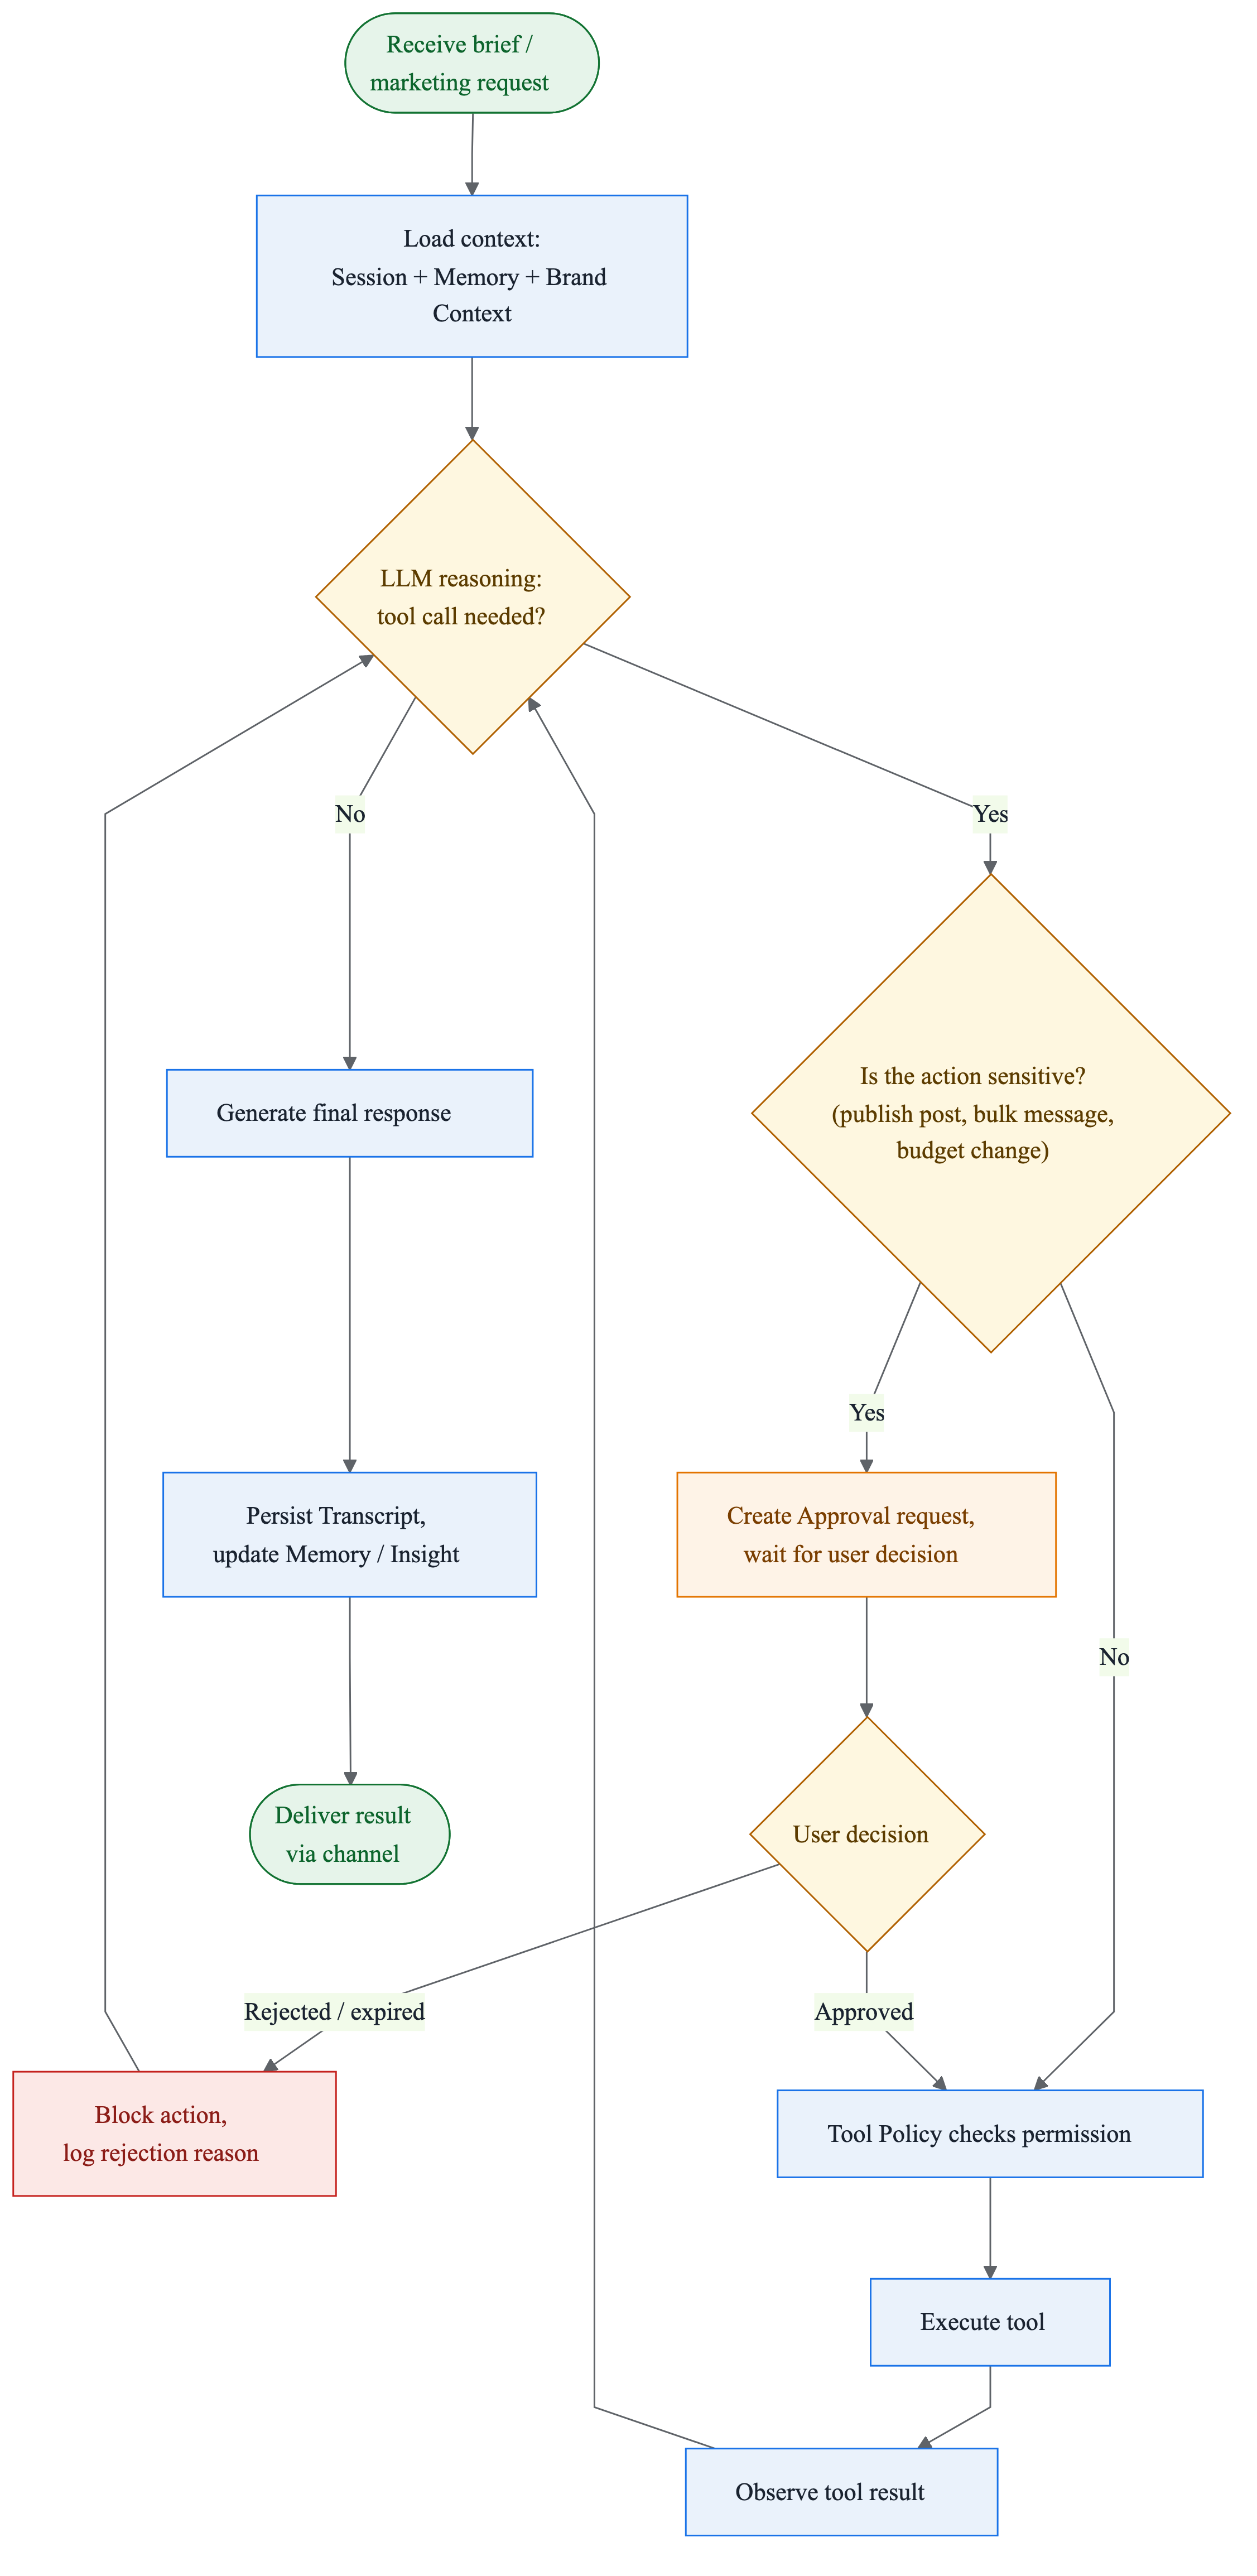
\includegraphics[width=0.78\textwidth,height=0.9\textheight,keepaspectratio]{media/figure_agent_react_loop.png}\caption{Luồng xử lý xuyên suốt của tác nhân: suy luận, gọi công cụ, phê duyệt và trả kết quả}\end{figure}

Vòng lặp trong Hình 3.14 dừng lại ở hai điều kiện: (1) \textit{điều kiện kết thúc bình thường} — khi mô hình xác định không còn cần gọi thêm công cụ, tác nhân sinh phản hồi cuối cùng, lưu Transcript và trả kết quả qua kênh giao tiếp; (2) \textit{điều kiện chặn} — khi hành động thuộc nhóm nhạy cảm nhưng người dùng từ chối hoặc để yêu cầu phê duyệt hết hạn, tác nhân không được phép thực thi hành động đó và phải quay lại bước suy luận với lý do bị từ chối.

Có thể minh họa luồng này bằng chính kịch bản Vinamilk Green Farm ở Chương 4 (Hình 4.2–4.8): người dùng gửi brief tạo bài đăng Facebook (nút \textit{Receive brief}); tác nhân nạp Brand Context đã lưu trước đó (nút \textit{Load context}, Hình 4.2); tác nhân xác định cần dùng công cụ tạo bản nháp (\textit{LLM reasoning} $\rightarrow$ \textit{Yes}), Tool Policy cho phép vì tạo bản nháp không phải hành động outbound (\textit{Tool Policy checks permission} $\rightarrow$ \textit{Execute tool}), kết quả là bản nháp ở trạng thái \texttt{draft} (Hình 4.4). Khi người dùng yêu cầu đăng bài ngay, tác nhân nhận ra đây là hành động nhạy cảm (\textit{Is the action sensitive?} $\rightarrow$ \textit{Yes}) nên tạo một bản ghi Approval và dừng lại chờ quyết định (nút \textit{Create Approval request}, Hình 4.5) thay vì tự ý đăng. Sau khi người dùng phản hồi \textit{"Duyệt nhé"} (\textit{User decision} $\rightarrow$ \textit{Approved}), tác nhân mới được phép tiếp tục lập lịch xử lý bản nháp (Hình 4.6) và cập nhật trạng thái chiến dịch (Hình 4.7).

Sau phần xương sống này, các hình con tiếp theo trong mục này trình bày chi tiết từng cơ chế được dùng lặp lại bên trong vòng lặp ở Hình 3.14: kiểm tra và thực thi công cụ, truy xuất bộ nhớ, lập lịch tác vụ định kỳ và ghi nhật ký vận hành. Hình 3.15 dưới đây trình bày lại luồng xử lý này ở mức hệ thống, theo từng lớp kiến trúc (Client, Gateway, Agent, Model, Storage), để đối chiếu với Hình 3.1.

\imgfig{media/imagef.png}{Sơ đồ tuần tự xử lý yêu cầu người dùng}

Một lượt xử lý yêu cầu được mô tả như sau:

\begin{enumerate}
\item Người dùng gửi yêu cầu từ dòng lệnh, giao diện web hoặc kênh giao tiếp đã cấu hình.
\item Client Layer hoặc Channel Adapter chuẩn hóa yêu cầu đầu vào.
\item Gateway Runtime kiểm tra người gửi, kênh, Session và thông tin chống xử lý trùng.
\item Hệ thống chuyển yêu cầu vào Agent Runtime.
\item Agent Runtime nạp Session, Workspace và Memory liên quan.
\item Hệ thống xây dựng prompt và danh sách công cụ được phép dùng.
\item Model Router chọn Model Provider và gửi yêu cầu đến mô hình ngôn ngữ lớn.
\item Nếu mô hình yêu cầu gọi công cụ, hệ thống kiểm tra Tool Policy, thực thi công cụ hợp lệ và đưa kết quả công cụ trở lại mô hình.
\item Mô hình tạo phản hồi cuối cùng cho người dùng.
\item Hệ thống lưu Transcript, thông tin Session và mức sử dụng mô hình.
\item Phản hồi được trả về Gateway Runtime.
\item Gateway Runtime gửi kết quả về kênh ban đầu.
\end{enumerate}

Khi mô hình yêu cầu gọi công cụ, hệ thống không thực thi ngay. Trước hết, công cụ phải tồn tại trong Tool Registry, tham số phải đúng cấu trúc và Tool Policy hiện tại phải cho phép sử dụng. Nếu công cụ không hợp lệ hoặc vượt quá quyền được phép, hệ thống từ chối thực thi hoặc yêu cầu người dùng xác nhận.

\imgfig{media/figure_3_15_tool_validation.png}{Luồng kiểm tra và thực thi lời gọi công cụ}

Luồng Memory Retrieval được dùng khi yêu cầu hiện tại cần sử dụng thông tin đã lưu trước đó. Ví dụ, khi tạo kế hoạch nội dung cho một sản phẩm, hệ thống có thể truy xuất thông tin về khách hàng mục tiêu, giọng văn, thông điệp đã dùng hoặc các ràng buộc cần tránh.

\begin{figure}[H]\centering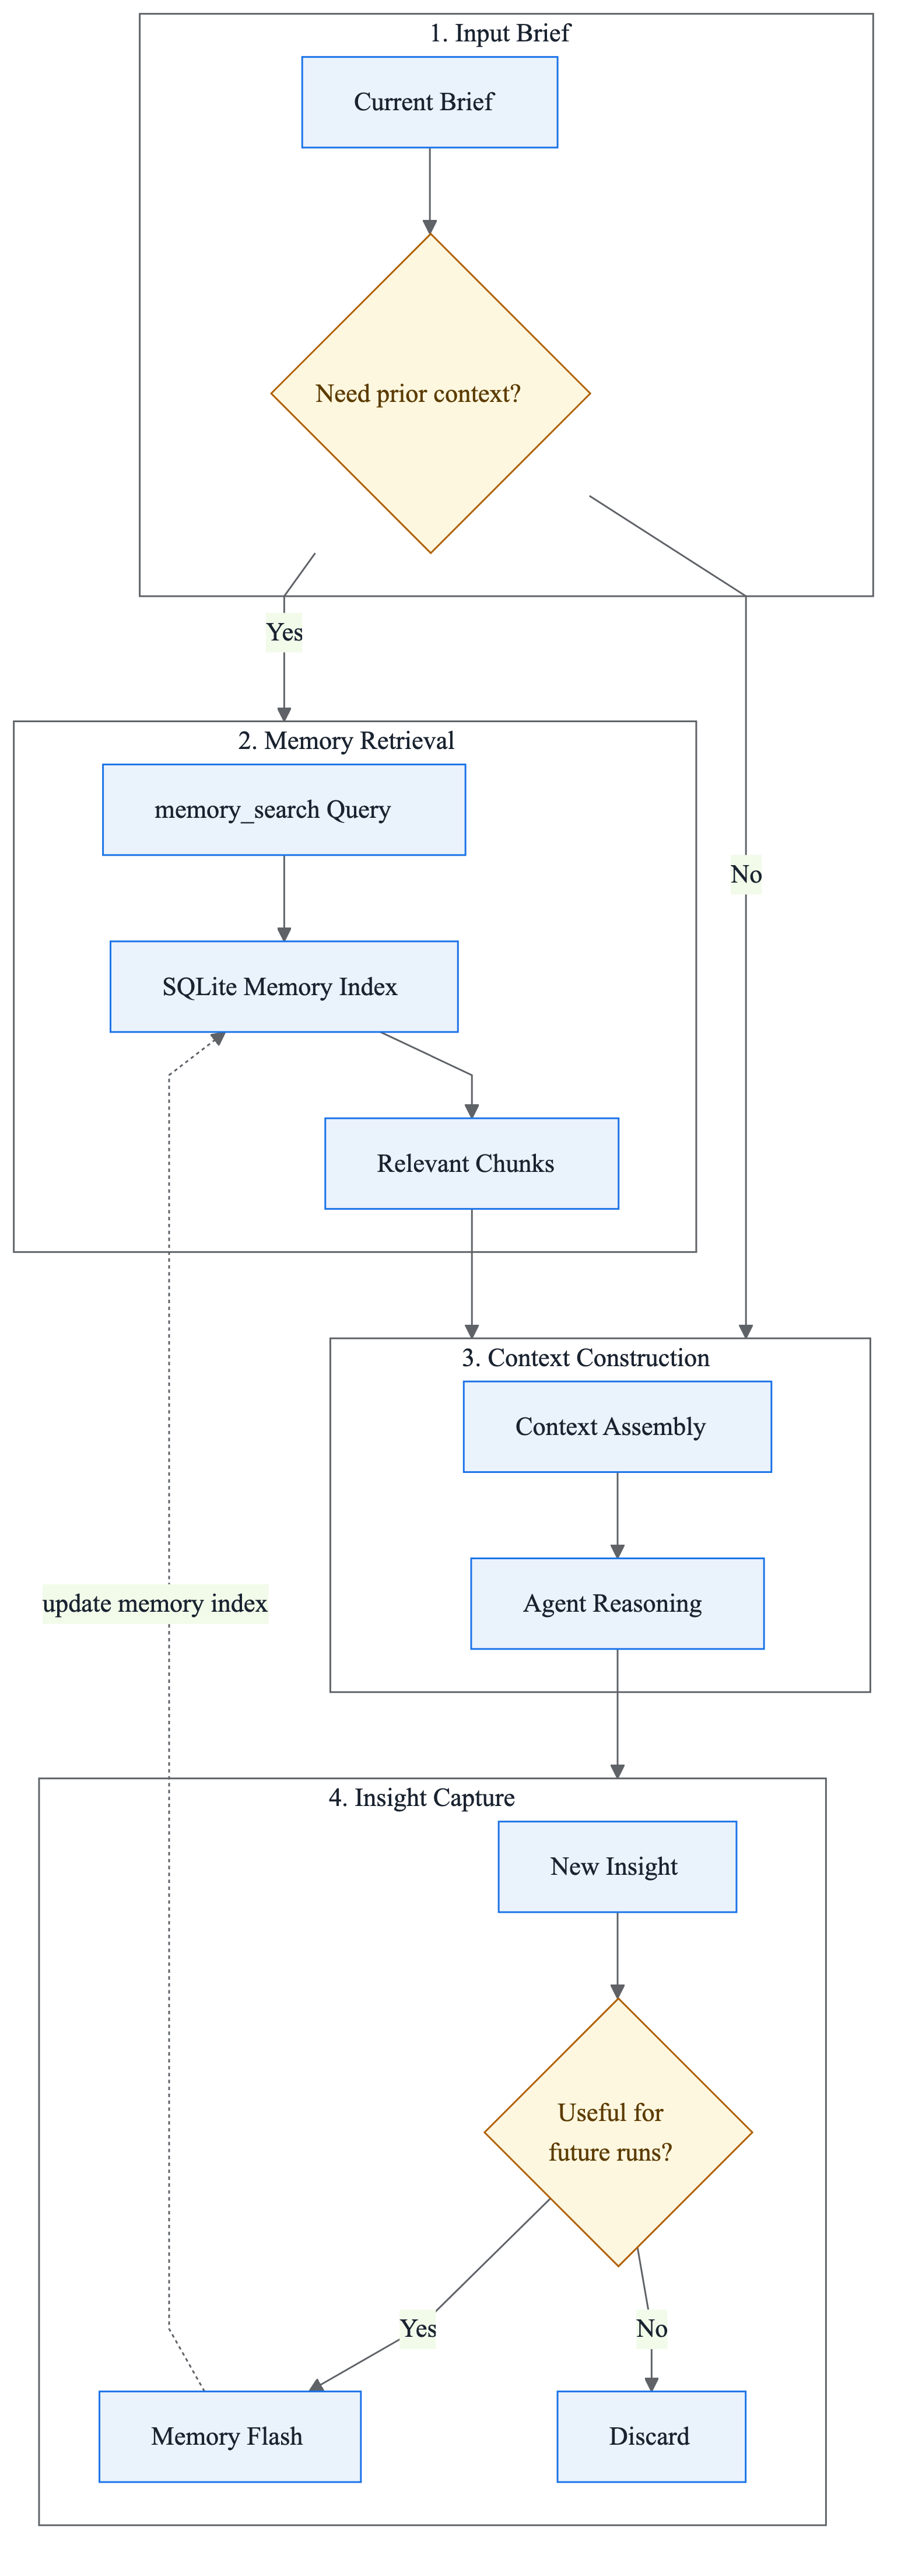
\includegraphics[width=0.6\textwidth,height=0.9\textheight,keepaspectratio]{media/figure_3_16_memory_retrieval.png}\caption{Luồng Memory Retrieval và cập nhật insight}\end{figure}

Scheduler được dùng cho các tác vụ có tính lặp lại như nhắc việc, tạo báo cáo tuần hoặc kiểm tra danh sách bản nháp. Khi tác vụ đến hạn, hệ thống tạo gói dữ liệu đầu vào và chuyển vào Agent Runtime như một yêu cầu thông thường. Nhờ đó, tác vụ định kỳ không chỉ là nhắc việc đơn giản mà có thể kích hoạt tác nhân tạo báo cáo hoặc gợi ý nội dung theo lịch.

\imgfig{media/figure_3_17_scheduler_design.png}{Luồng thiết kế Scheduler và tác vụ định kỳ}

\begin{figure}[H]\centering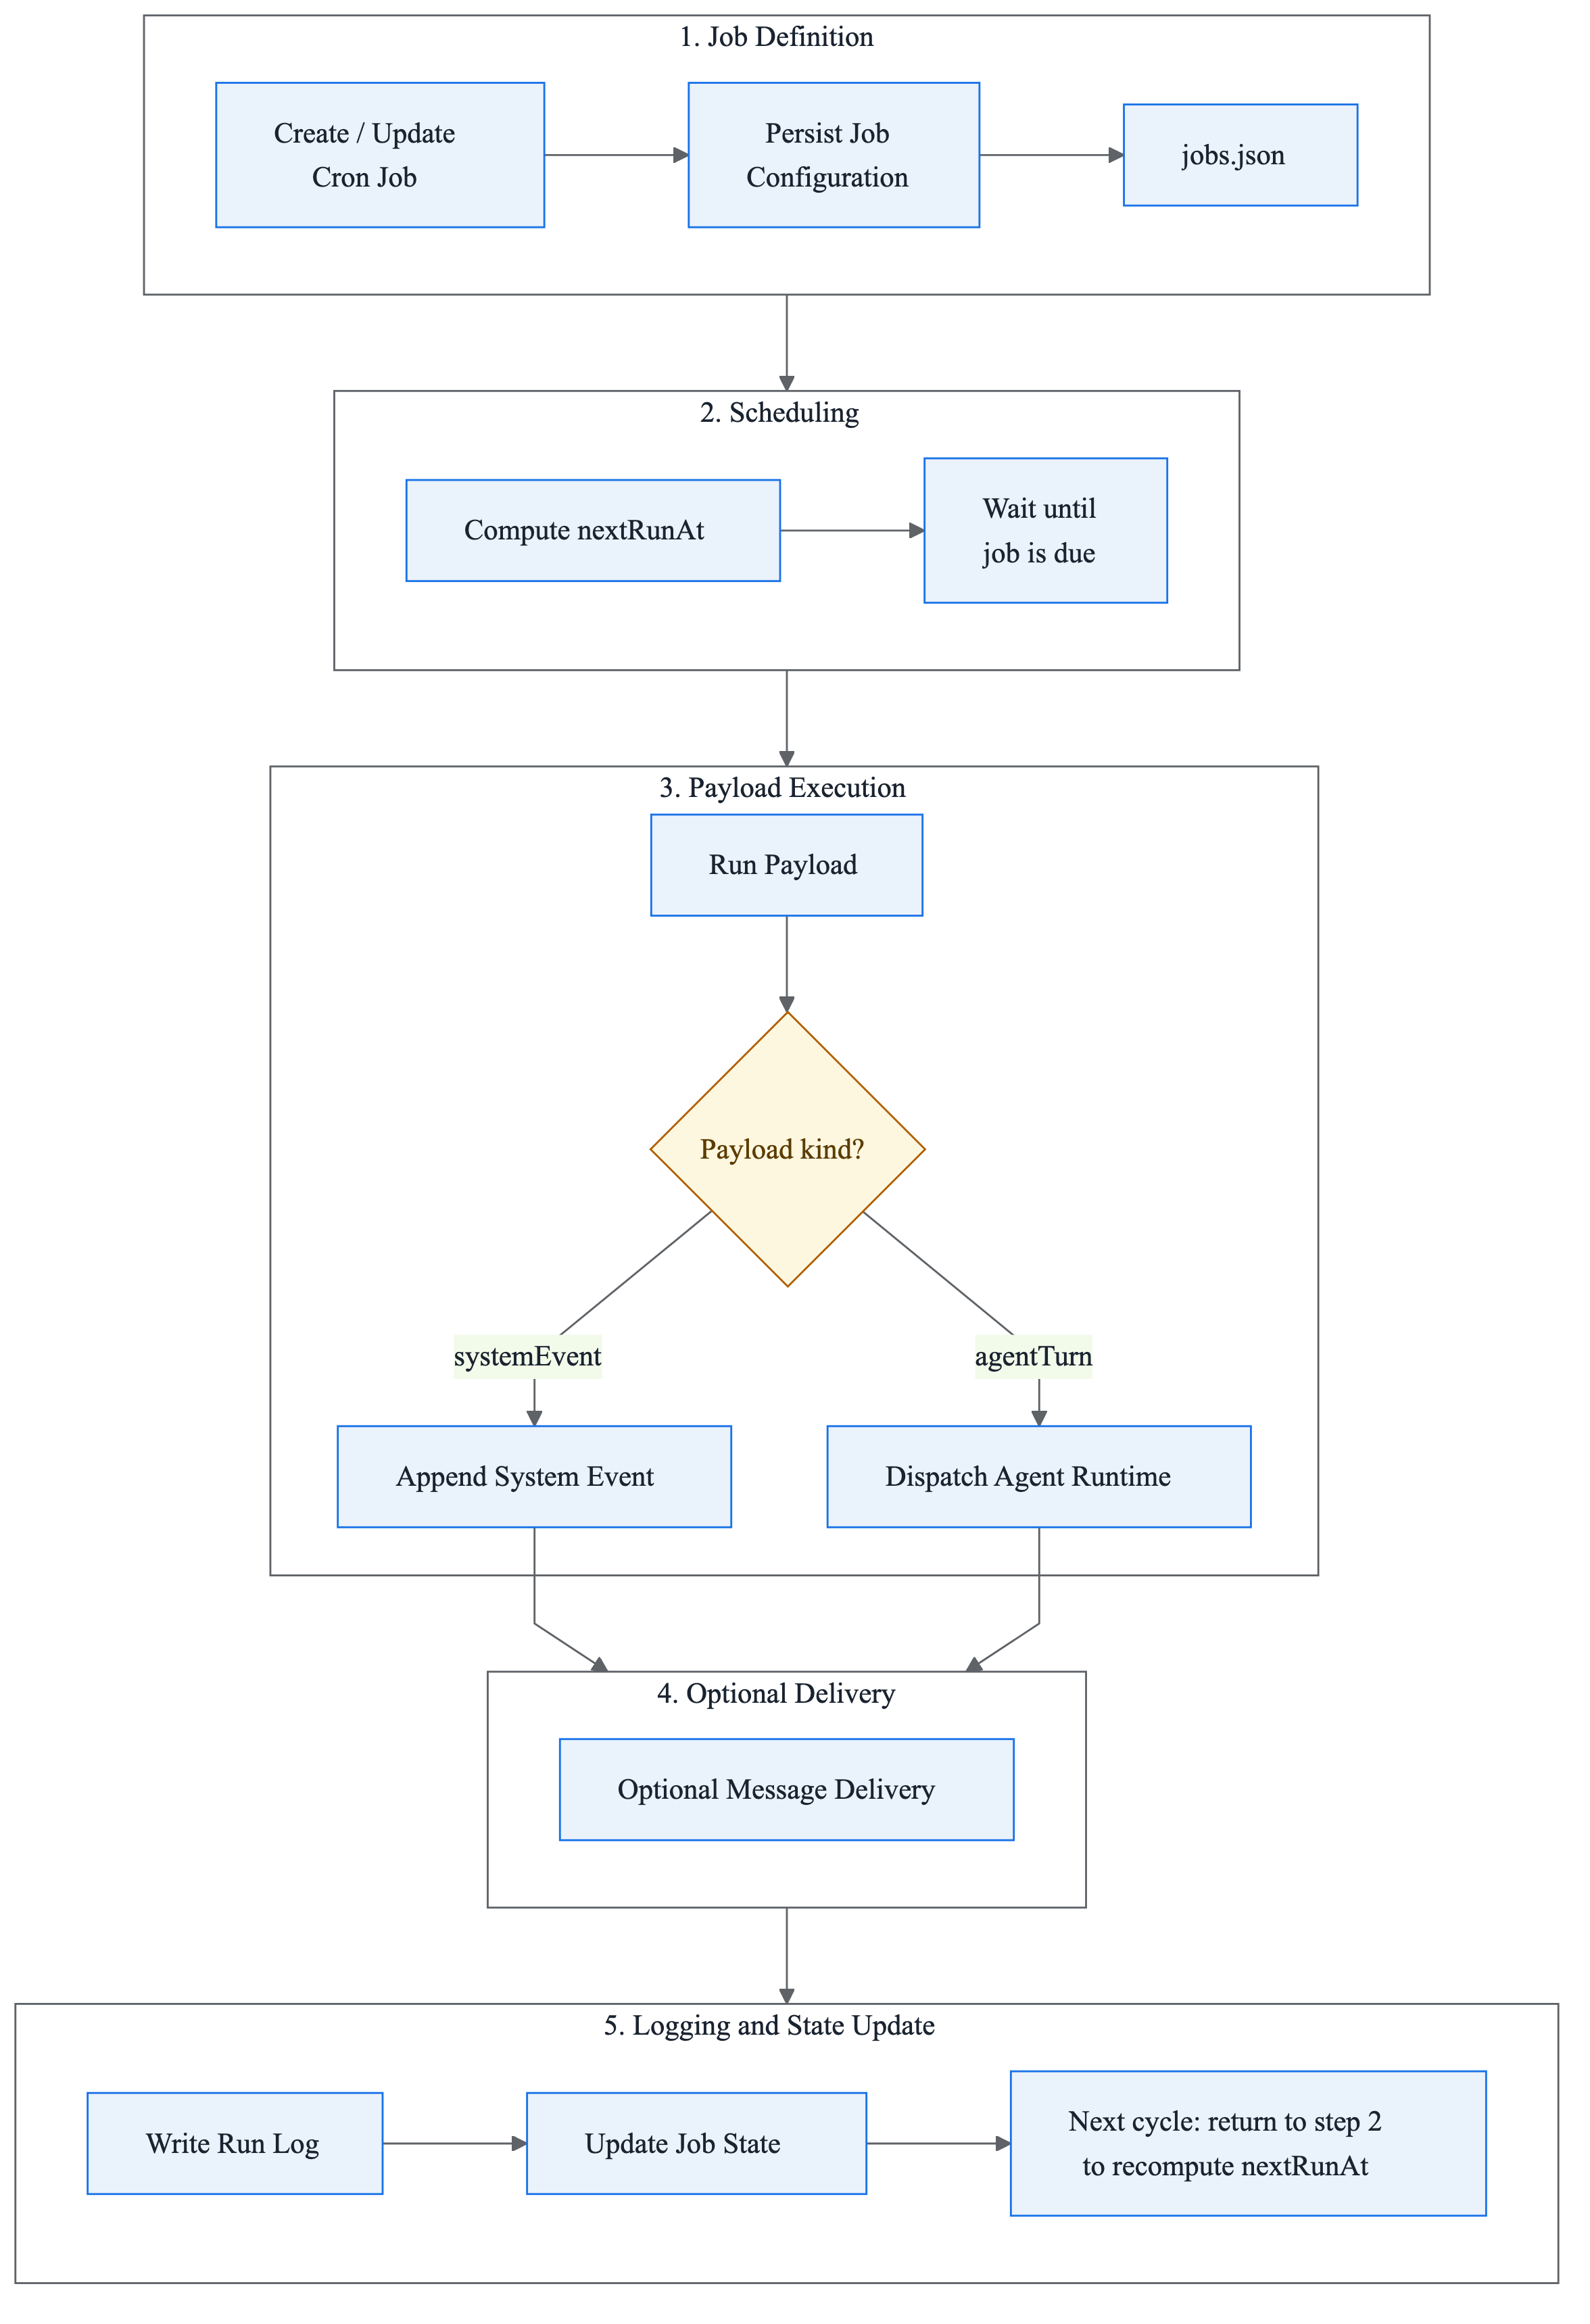
\includegraphics[width=0.85\textwidth,height=0.9\textheight,keepaspectratio]{media/figure_3_18_cron_run.png}\caption{Luồng chạy tác vụ định kỳ và cập nhật trạng thái}\end{figure}

Sau khi Agent Runtime tạo kết quả, phản hồi được gửi về kênh ban đầu thông qua Gateway Runtime và Channel Adapter. Với các kênh bên ngoài, hệ thống cần kiểm tra người nhận, kênh đích và quyền gửi để hạn chế rủi ro gửi nhầm thông tin.

\imgfig{media/figure_3_19_response_delivery.png}{Luồng phản hồi qua kênh giao tiếp}

Hệ thống cũng lưu lại Transcript, lượt gọi công cụ, mức sử dụng mô hình và nhật ký chạy tác vụ định kỳ. Các dữ liệu này giúp kiểm tra lỗi, theo dõi lịch sử xử lý và đánh giá hiệu quả của hệ thống. Ví dụ, nếu một yêu cầu không được xử lý đúng, người phụ trách có thể xem lại Transcript để hiểu diễn biến và xác định nguyên nhân.

\imgfig{media/figure_3_20_logging.png}{Luồng ghi nhật ký, mức sử dụng và trạng thái vận hành}

\subsecx{3.3.7. Thiết kế kiểm soát hành động và an toàn}

Do hệ thống tác nhân có thể sử dụng công cụ và tương tác với dữ liệu bên ngoài, thiết kế kiểm soát hành động là phần bắt buộc. Trong phạm vi đồ án, hệ thống không tự động thực hiện các thao tác có ảnh hưởng trực tiếp ra bên ngoài nếu chưa có sự kiểm tra hoặc phê duyệt của người dùng.

Hệ thống áp dụng ba nguyên tắc chính. Thứ nhất, đọc và phân tích dữ liệu trước khi thực hiện hành động ghi. Thứ hai, tạo bản nháp trước khi gửi hoặc đăng nội dung. Thứ ba, các thao tác có rủi ro như gửi nội dung, đăng bài, ghi dữ liệu hoặc gọi API nhạy cảm cần được xác nhận trước khi thực hiện.

Các nguyên tắc này giúp hệ thống giữ đúng vai trò hỗ trợ người dùng. Tác nhân có thể đề xuất nội dung, tổng hợp thông tin hoặc tạo báo cáo, nhưng quyền quyết định cuối cùng vẫn thuộc về người phụ trách.

\renewcommand{\arraystretch}{1.25}
\begin{longtable}{L{0.23\textwidth}L{0.32\textwidth}L{0.35\textwidth}}
\caption{Rủi ro và biện pháp kiểm soát}\\
\toprule
\textbf{Rủi ro} & \textbf{Mô tả} & \textbf{Biện pháp}\\
\midrule
\endfirsthead
\toprule
\textbf{Rủi ro} & \textbf{Mô tả} & \textbf{Biện pháp}\\
\midrule
\endhead

Chèn lệnh vào lời nhắc & Nội dung đầu vào hoặc dữ liệu ngoài yêu cầu mô hình bỏ qua chính sách hệ thống. & Tách hướng dẫn hệ thống, giới hạn công cụ được phép dùng và không tin hoàn toàn dữ liệu ngoài.\\

Lộ thông tin xác thực & Khóa API hoặc thông tin xác thực bị đưa vào lời nhắc, Transcript hoặc nhật ký chạy. & Dùng tham chiếu bí mật, che log và không chèn trực tiếp thông tin xác thực vào ngữ cảnh gửi cho mô hình.\\

Gửi nhầm kênh & Báo cáo, bản nháp hoặc thông báo được gửi sai người nhận hoặc sai kênh. & Kiểm tra kênh đích, người nhận và yêu cầu xác nhận trước khi gửi ra bên ngoài.\\

Ghi dữ liệu ngoài ý muốn & Công cụ ghi tệp, cập nhật dữ liệu hoặc gọi API khi chưa được phép. & Kiểm tra quyền công cụ và áp dụng quy tắc phê duyệt trước khi ghi dữ liệu.\\

Nội dung không nhất quán & Bản nháp không bám thông tin thương hiệu, giọng văn hoặc ràng buộc đã lưu. & Truy xuất Memory và lắp ráp ngữ cảnh trước khi sinh nội dung.\\

\bottomrule
\end{longtable}
\renewcommand{\arraystretch}{1}

Trọng tâm của cơ chế kiểm soát là cổng phê duyệt (\textit{approval gate}) đặt trước mọi hành động ghi hoặc gửi ra bên ngoài. Cổng này được hiện thực trong mô-đun kiểm soát phê duyệt của lớp marketing và quyết định một hành động có được phép thực hiện hay không dựa trên loại hành động, trạng thái bản nháp và trạng thái yêu cầu phê duyệt liên quan. Đoạn mã giả dưới đây mô tả logic ra quyết định của cổng phê duyệt.

\begin{lstlisting}[caption={Logic ra quyết định của cổng phê duyệt (approval gate)},captionpos=b]
// Write/outbound actions that require approval
WRITE_ACTIONS = { publish_post, bulk_message,
                  ads_write, integration_write }
// Draft statuses allowed to be published
PUBLISHABLE_STATUSES = { approved, scheduled }

function checkApprovalGate(action, draft, approval):
    // 1. Non-sensitive actions are allowed immediately
    if action.kind not in WRITE_ACTIONS:
        return ALLOW

    // 2. Draft must be in a publishable status
    if draft.status not in PUBLISHABLE_STATUSES:
        return BLOCK("draft status must be approved or scheduled")

    // 3. Draft must be linked to an approval request
    if draft.approvalId is empty:
        return BLOCK("draft has no linked approval")

    // 4. Approval must exist and match this draft
    if approval is null or approval.id != draft.approvalId:
        return BLOCK("approval record not found for this draft")

    // 5. Approval must be granted by the user
    if approval.status != approved:
        return BLOCK("approval status must be approved")

    // Allow the write/outbound action only after all five checks pass
    return ALLOW
\end{lstlisting}

Logic trên cho thấy mặc định an toàn của hệ thống: chỉ khi đồng thời thỏa mãn cả năm điều kiện thì hành động ghi hoặc gửi mới được phép, còn lại đều bị chặn. Hành động không nhạy cảm như tạo bản nháp, tổng hợp thông tin hoặc đọc số liệu được cho qua ngay ở bước một, nên cơ chế kiểm soát không cản trở các tác vụ hỗ trợ thông thường. Cách tổ chức này hiện thực trực tiếp nguyên tắc đọc trước, tạo bản nháp trước, phê duyệt trước khi ghi ra bên ngoài đã nêu ở mục 2.2.5, và là điểm khác biệt chính so với các công cụ chỉ sinh nội dung hoặc tự động hóa theo kịch bản cố định.


\secx{3.4. Kết luận chương}

Chương này đã trình bày phương pháp nghiên cứu, phân tích yêu cầu và thiết kế hệ thống tác nhân tự chủ hỗ trợ vận hành marketing số. Nội dung chương đã xác định nhóm người dùng hướng đến, các chức năng nghiệp vụ, các thành phần bên trong của hệ thống tác nhân và các yêu cầu phi chức năng cần đáp ứng.

Phần thiết kế hệ thống đã trình bày kiến trúc tổng thể, các thành phần chính của tác nhân, Memory, Session, Storage Layer, Channel Adapter, luồng xử lý và cơ chế kiểm soát hành động.



\setcounter{chapnum}{4}
\setcounter{figure}{0}
\setcounter{table}{0}
\chap{CHƯƠNG 4: HIỆN THỰC VÀ KẾT QUẢ}

\secx{4.1. Môi trường phát triển}

Hệ thống được hiện thực trong môi trường phát triển cục bộ. Mã nguồn được viết chủ yếu bằng TypeScript và chạy trên Node.js. Công cụ pnpm được sử dụng để cài đặt thư viện, quản lý các gói phụ thuộc và chạy các lệnh phát triển. Vitest được sử dụng để kiểm thử một số module chính của hệ thống.

\renewcommand{\arraystretch}{1.25}
\begin{longtable}{L{0.30\textwidth}L{0.60\textwidth}}
\caption{Môi trường, công cụ và dữ liệu sử dụng}\\
\toprule
\textbf{Thành phần} & \textbf{Vai trò trong đồ án}\\
\midrule
\endfirsthead
\toprule
\textbf{Thành phần} & \textbf{Vai trò trong đồ án}\\
\midrule
\endhead

TypeScript & Ngôn ngữ lập trình chính dùng để hiện thực các module của hệ thống.\\

Node.js & Môi trường chạy cho \textit{Agent Runtime}, \textit{Gateway Runtime}, công cụ và tác vụ nền.\\

pnpm & Công cụ quản lý thư viện, cài đặt phụ thuộc và chạy các lệnh phát triển.\\

Vitest & Công cụ kiểm thử các module TypeScript trong hệ thống.\\

Markdown & Định dạng lưu các thông tin cần dễ đọc và dễ chỉnh sửa thủ công, như ghi nhớ dài hạn hoặc thông tin ngữ cảnh.\\

JSON/JSONL & Định dạng lưu cấu hình, transcript, dữ liệu phiên và log chạy tác vụ.\\

SQLite & Cơ sở dữ liệu gọn nhẹ dùng để hỗ trợ chỉ mục tìm kiếm cho \textit{Memory}.\\

Docker & Công cụ hỗ trợ đóng gói và chạy hệ thống trong môi trường ổn định hơn khi cần.\\

\bottomrule
\end{longtable}
\renewcommand{\arraystretch}{1}

\secx{4.2. Kết quả đạt được}

Kết quả đạt được được trình bày theo hai phần: kết quả chạy chương trình và đánh giá kết quả so với mục tiêu đã đặt ra. Các kết quả trong chương này được hiểu là kết quả kỹ thuật trong môi trường phát triển, chưa phải kết quả triển khai trên một chiến dịch marketing thật.

\subsecx{4.2.1. Kết quả chạy chương trình}

Sau khi hiện thực, hệ thống đã chạy được các luồng chức năng chính của một tác nhân hỗ trợ vận hành marketing số. Luồng đại diện gồm: lưu thông tin thương hiệu, tạo bản nháp nội dung, chỉnh sửa nội dung theo kênh, yêu cầu phê duyệt, kiểm soát hành động gửi ra bên ngoài và xử lý các bản nháp đã đến lịch.

\renewcommand{\arraystretch}{1.25}
\begin{longtable}{L{0.28\textwidth}L{0.62\textwidth}}
\caption{Kết quả chạy chương trình theo nhóm chức năng}\\
\toprule
\textbf{Nhóm kết quả} & \textbf{Kết quả đạt được}\\
\midrule
\endfirsthead
\toprule
\textbf{Nhóm kết quả} & \textbf{Kết quả đạt được}\\
\midrule
\endhead

Lưu ngữ cảnh marketing & Hệ thống lưu được thông tin thương hiệu, sản phẩm, khách hàng mục tiêu, giọng văn và ràng buộc nội dung.\\

Tạo bản nháp nội dung & Hệ thống tạo được bản nháp nội dung và lưu bản nháp ở trạng thái ban đầu, chưa tự động gửi hoặc đăng ra bên ngoài.\\

Chỉnh sửa theo kênh & Nội dung có thể được chuyển thành các biến thể phù hợp hơn với từng kênh, ví dụ rút gọn nội dung hoặc điều chỉnh định dạng.\\

Quản lý phê duyệt & Bản nháp có thể được chuyển sang trạng thái chờ duyệt và chỉ được xử lý tiếp khi có phê duyệt hợp lệ.\\

Kiểm soát hành động gửi ra ngoài & Hệ thống chặn các hành động gửi hoặc đăng nội dung khi bản nháp chưa được phê duyệt.\\

Lập lịch & Hệ thống xác định được các bản nháp đã được duyệt, đã đặt lịch và đã đến thời điểm xử lý.\\

Tác vụ định kỳ & Hệ thống hỗ trợ tạo và xử lý một số tác vụ định kỳ, đồng thời ghi lại log chạy tác vụ.\\

\bottomrule
\end{longtable}
\renewcommand{\arraystretch}{1}

Một luồng chạy thử đại diện của hệ thống gồm các bước sau:

\begin{enumerate}
\item Người dùng cung cấp thông tin thương hiệu, sản phẩm, khách hàng mục tiêu và ràng buộc nội dung.
\item Hệ thống lưu các thông tin này vào ngữ cảnh marketing.
\item Người dùng yêu cầu tạo bản nháp nội dung cho nền tảng cần sử dụng.
\item Hệ thống tạo bản nháp và lưu ở trạng thái chưa phê duyệt.
\item Khi có yêu cầu gửi hoặc đăng nội dung, hệ thống kiểm tra trạng thái phê duyệt.
\item Nếu bản nháp chưa được duyệt, hệ thống không gửi ra bên ngoài mà yêu cầu phê duyệt trước.
\item Sau khi bản nháp được duyệt và đặt lịch, hệ thống có thể liệt kê các bản nháp đã đến thời điểm xử lý.
\end{enumerate}

Các hình dưới đây minh họa một phiên chạy thử qua kênh Telegram. Phiên chạy thử sử dụng dữ liệu giả lập cho thương hiệu Vinamilk Green Farm để thể hiện các bước chính của luồng vận hành: nhận yêu cầu, lưu ngữ cảnh thương hiệu, phân tích campaign brief, tạo bản nháp, kiểm soát phê duyệt, ghi nhận lịch xử lý, theo dõi trạng thái campaign và tạo báo cáo ngắn từ số liệu được cung cấp.

\imgfig{media/demo-agent.png}{Giao diện Telegram khi người dùng tương tác với tác nhân hỗ trợ vận hành marketing}

\imgfig{media/save-brand-context.png}{Tác nhân ghi nhận Brand Context và các ràng buộc nội dung}

\imgfig{media/create-campaign-brief.png}{Tác nhân tạo campaign brief từ yêu cầu của người dùng}

\imgfig{media/create-draft.png}{Tác nhân tạo bản nháp bài đăng theo ngữ cảnh thương hiệu}

\imgfig{media/check-approval.png}{Tác nhân yêu cầu phê duyệt trước khi thực hiện hành động đăng nội dung}

\imgfig{media/approved-scheduled.png}{Tác nhân ghi nhận phê duyệt và lập lịch xử lý bản nháp}

\imgfig{media/status-campaign.png}{Tác nhân tổng hợp trạng thái campaign sau khi tạo bản nháp, phê duyệt và lập lịch}

\imgfig{media/report.png}{Tác nhân tạo báo cáo ngắn từ số liệu marketing giả lập}

Kết quả trên cho thấy hệ thống đã hiện thực được các thành phần nền tảng để hỗ trợ quy trình marketing có trạng thái và có kiểm soát. Điểm quan trọng là hệ thống không chỉ tạo nội dung, mà còn quản lý được ngữ cảnh, trạng thái bản nháp, lịch xử lý và điều kiện phê duyệt.

\subsecx{4.2.2. Đánh giá kết quả}

So với mục tiêu ban đầu, hệ thống đã đáp ứng được các yêu cầu ở mức nền tảng. Hệ thống có thể lưu thông tin thương hiệu, tạo bản nháp nội dung, chỉnh sửa nội dung theo kênh, lập lịch, tạo tác vụ định kỳ và kiểm soát các hành động cần phê duyệt. Các thành phần như \textit{Session}, \textit{Memory}, \textit{Tool Policy}, \textit{Scheduler} và \textit{Gateway Runtime} giúp hệ thống hoạt động giống một tác nhân có trạng thái hơn là một công cụ trả lời từng lượt.

Tuy nhiên, kết quả hiện tại vẫn có giới hạn. Hệ thống mới được kiểm tra bằng dữ liệu mẫu và kịch bản giả lập, chưa triển khai trên dữ liệu chiến dịch thật trong thời gian dài. Chất lượng nội dung do mô hình sinh ra cũng chưa được đánh giá bằng người dùng thật hoặc chỉ số kinh doanh. Các chức năng như lấy dữ liệu quảng cáo trực tiếp từ nền tảng, tự động đăng bài sau phê duyệt, đánh giá hiệu quả nội dung và tối ưu ngân sách quảng cáo vẫn thuộc hướng phát triển tiếp theo.

\subsecx{4.2.3. Ánh xạ mục tiêu, chức năng, hiện thực và kiểm thử}

Để làm rõ mức độ hoàn thành của đồ án, phần này tổng hợp mối quan hệ giữa mục tiêu nghiên cứu, nhóm chức năng, phần hiện thực và kết quả kiểm thử. Cách trình bày này giúp phân biệt các nội dung đã được hiện thực trong phạm vi đồ án, các nội dung mới dừng ở mức hỗ trợ nền tảng và các nội dung được xác định là hướng phát triển tiếp theo.

\renewcommand{\arraystretch}{1.22} \begin{longtable}{L{0.15\textwidth}L{0.15\textwidth}L{0.19\textwidth}L{0.15\textwidth}L{0.10\textwidth}L{0.10\textwidth}} \caption{Ánh xạ mục tiêu, chức năng, hiện thực và kiểm thử} \label{tab:anh-xa-muc-tieu-chuc-nang-hien-thuc-kiem-thu}\\ \toprule \textbf{Mục tiêu hoặc phạm vi} & \textbf{Chức năng liên quan} & \textbf{Hiện thực trong đồ án} & \textbf{Kiểm thử hoặc minh chứng} & \textbf{Trạng thái} & \textbf{Kế thừa / Tự xây}\\ \midrule \endfirsthead \toprule \textbf{Mục tiêu hoặc phạm vi} & \textbf{Chức năng liên quan} & \textbf{Hiện thực trong đồ án} & \textbf{Kiểm thử hoặc minh chứng} & \textbf{Trạng thái} & \textbf{Kế thừa / Tự xây}\\ \midrule \endhead Xác định phạm vi hỗ trợ vận hành marketing số & Phân tích yêu cầu marketing, xác định nhóm người dùng và nhóm công việc cần hỗ trợ & Đã phân tách chức năng nghiệp vụ marketing với các thành phần kỹ thuật nền của tác nhân & Thể hiện qua phân tích yêu cầu, bảng chức năng nghiệp vụ và các kịch bản kiểm thử giả lập & Hoàn thành ở mức phân tích và thiết kế & Tự xây\\ Tổ chức hệ thống tác nhân có trạng thái & Session, Memory, Tool Policy, Scheduler, Gateway Runtime và plugin & Đã sử dụng các thành phần nền để duy trì ngữ cảnh, quản lý phiên, lọc công cụ, chạy tác vụ định kỳ và tiếp nhận yêu cầu qua gateway & Nhóm kiểm thử Agent Runtime, Gateway, kênh, plugin, Memory và Provider đều đạt trong bộ kiểm thử & Hoàn thành ở mức nền tảng kỹ thuật & Kế thừa\\ Hỗ trợ ngữ cảnh marketing & Lưu thông tin thương hiệu, sản phẩm, khách hàng mục tiêu và ràng buộc nội dung & Đã có lớp dữ liệu marketing và cơ chế nạp ngữ cảnh thương hiệu cho tác nhân & Nhóm kiểm thử Marketing kiểm tra ngữ cảnh thương hiệu và dữ liệu bản nháp & Hoàn thành ở mức thử nghiệm & Tự xây\\ Tạo và điều chỉnh nội dung marketing & Tạo bản nháp nội dung, tạo biến thể và chỉnh sửa theo kênh & Đã hiện thực vòng đời bản nháp, gồm tạo bản nháp, lưu trạng thái, chỉnh sửa theo kênh và chuẩn bị nội dung để người dùng duyệt & Nhóm kiểm thử Marketing kiểm tra bản nháp, biến thể nội dung và trạng thái xử lý & Hoàn thành ở mức bản nháp hỗ trợ & Tự xây\\ Kiểm soát thao tác có rủi ro & Yêu cầu phê duyệt, xử lý phê duyệt và chặn gửi ra ngoài khi chưa đủ điều kiện & Đã áp dụng nguyên tắc tạo bản nháp trước và phê duyệt trước khi ghi hoặc gửi ra bên ngoài & Kiểm thử Marketing và kiểm thử chính sách công cụ xác minh các trường hợp chưa được phép gửi & Hoàn thành ở mức kiểm soát logic & Kết hợp\\ Lập lịch và tác vụ định kỳ & Lập lịch bản nháp, xác định bản nháp đến hạn và tạo tác vụ lặp lại & Đã có cơ chế xác định bản nháp đã duyệt, đã đặt lịch, đã đến thời điểm xử lý và ghi nhận nhật ký chạy tác vụ & Nhóm kiểm thử Scheduler và log đạt 63/63 testcase & Hoàn thành ở mức nền tảng & Kết hợp\\ Tạo báo cáo và tổng hợp thông tin & Tóm tắt dữ liệu đầu vào, công việc đã làm và điểm cần chú ý & Đã mô tả và kiểm tra ở mức tác nhân có thể tạo bản nháp báo cáo từ dữ liệu được cung cấp hoặc trạng thái có sẵn & Được kiểm chứng ở mức kịch bản giả lập và nhóm kiểm thử chức năng marketing & Hoàn thành ở mức hỗ trợ & Tự xây\\ Nghiên cứu thị trường, phân tích quảng cáo và phối hợp nhóm & Hỗ trợ nghiên cứu, đọc số liệu quảng cáo, gửi bản nháp hoặc thông báo vào kênh làm việc & Đã định nghĩa trong phạm vi chức năng và có nền tảng công cụ, kênh, gateway để hỗ trợ; chưa đánh giá bằng dữ liệu chiến dịch thật hoặc tích hợp quảng cáo đầy đủ & Được mô tả trong đánh giá kết quả và hạn chế; các tích hợp dữ liệu thật được đưa vào hướng phát triển & Một phần ở mức hỗ trợ, phần nâng cao là hướng phát triển & Kết hợp\\ Đánh giá mức độ đáp ứng mục tiêu & Kiểm thử theo kịch bản sử dụng giả lập và tổng hợp kết quả & Đã tổng hợp 308 testcase, gồm 247 testcase thuộc các thành phần nền kế thừa và 61 testcase thuộc chức năng marketing tự xây & Kết quả kiểm thử 308/308 testcase đạt trong môi trường phát triển & Hoàn thành trong phạm vi kiểm thử giả lập & Kết hợp\\ \bottomrule \end{longtable} \renewcommand{\arraystretch}{1}

Từ Bảng trên, có thể thấy phần đã hoàn thành của đồ án tập trung vào nền tảng kỹ thuật của hệ thống tác nhân, quản lý ngữ cảnh, tạo bản nháp, phê duyệt, kiểm soát thao tác và lập lịch. Các nội dung liên quan đến dữ liệu thị trường theo thời gian thực, tích hợp quảng cáo trực tiếp, đánh giá chất lượng nội dung bằng người dùng thật và tối ưu hiệu quả kinh doanh chưa được xem là kết quả đã hoàn thành, mà được tách rõ sang phần hạn chế và hướng phát triển

\secx{4.3. Kiểm thử}

Kiểm thử được thực hiện nhằm xác minh các chức năng chính và các cơ chế kiểm soát của hệ thống. Bộ kiểm thử tập trung vào hai nhóm: nhóm chức năng marketing và nhóm thành phần nền của hệ thống tác nhân.

Nhóm chức năng marketing kiểm tra việc lưu ngữ cảnh thương hiệu, tạo bản nháp, chỉnh sửa nội dung theo kênh, quản lý phê duyệt, kiểm soát hành động gửi ra ngoài và lập lịch. Nhóm thành phần nền kiểm tra \textit{Scheduler}, \textit{Tool Policy}, \textit{Memory}, \textit{Gateway Runtime}, plugin và các thành phần liên quan đến vận hành tác nhân.

Kết quả kiểm thử cho thấy 308/308 testcase được chọn đều đạt trong môi trường phát triển. Kết quả này cho thấy các module chính hoạt động đúng theo các trường hợp kiểm thử đã xây dựng. Để phản ánh đúng ranh giới đóng góp, bảng tóm tắt dưới đây tách riêng 247 testcase thuộc các nhóm thành phần nền được kế thừa từ nền tảng OpenClaw và 61 testcase thuộc nhóm chức năng marketing do đồ án tự xây dựng. Năm nhóm thành phần trong bảng được tổng hợp từ 18 nhóm kiểm thử chi tiết theo mã định danh testcase (xem Phụ lục B).

\renewcommand{\arraystretch}{1.25}
\begin{longtable}{L{0.24\textwidth}L{0.30\textwidth}L{0.08\textwidth}L{0.08\textwidth}L{0.14\textwidth}}
\caption{Tóm tắt kết quả kiểm thử}\\
\toprule
\textbf{Nhóm kiểm thử} & \textbf{Nội dung kiểm thử} & \textbf{Tổng} & \textbf{Đạt} & \textbf{Kế thừa / Tự xây}\\
\midrule
\endfirsthead
\toprule
\textbf{Nhóm kiểm thử} & \textbf{Nội dung kiểm thử} & \textbf{Tổng} & \textbf{Đạt} & \textbf{Kế thừa / Tự xây}\\
\midrule
\endhead

Agent runtime & Chính sách công cụ, kỹ năng workspace, tác nhân con, phát hiện vòng lặp công cụ và theo dõi thay đổi. & 95 & 95 & Kế thừa\\
Scheduler và log & Tác vụ định kỳ, lịch chạy và log chạy tác vụ. & 63 & 63 & Kế thừa\\
Gateway, kênh và bảo mật & Kênh giao tiếp, giám sát trạng thái kênh và xác thực gateway. & 51 & 51 & Kế thừa\\
Plugin, Memory và Provider & Plugin bộ nhớ, provider mô hình và các thành phần mở rộng. & 38 & 38 & Kế thừa\\
\midrule
\textbf{Tổng nhóm nền (kế thừa)} & Các thành phần nền kế thừa từ nền tảng OpenClaw. & \textbf{247} & \textbf{247} & Kế thừa\\
\midrule
Marketing & Ngữ cảnh thương hiệu, bản nháp, chỉnh sửa theo kênh, phê duyệt và kiểm soát gửi ra ngoài. & 61 & 61 & Tự xây\\
\textbf{Tổng nhóm marketing (tự xây)} & Phần chức năng marketing do đồ án tự xây dựng trên nền tảng kế thừa. & \textbf{61} & \textbf{61} & Tự xây\\
\midrule
\textbf{Tổng cộng} & & \textbf{308} & \textbf{308} & \\
\bottomrule
\end{longtable}
\renewcommand{\arraystretch}{1}

Kết quả kiểm thử cho thấy các chức năng của hệ thống hoạt động đúng trong phạm vi kiểm thử. Đặc biệt, các cơ chế như phê duyệt trước khi gửi, chặn hành động chưa được phép và kiểm soát công cụ được kiểm tra ở nhiều trường hợp khác nhau.

Điểm 308/308 chỉ nói lên rằng các testcase đã chọn đều đạt, chứ chưa tự nó chứng minh bộ kiểm thử có phủ đủ các tình huống ngoài đường thành công hay không. Vì vậy, thay vì chỉ dừng ở kiểm thử "hệ thống có chạy được hay không", nhóm 61 testcase chức năng marketing được thiết kế theo bốn loại: đường thành công, tình huống biên (thông tin đầu vào thiếu), tình huống phải từ chối (yêu cầu đăng bài khi chưa duyệt, yêu cầu vi phạm guardrail thương hiệu) và chuyển trạng thái không hợp lệ (bỏ qua bước phê duyệt). Phụ lục B trình bày bảy testcase tiêu biểu theo bốn loại này kèm Pre-condition, Test Data và Expected results cụ thể, nhằm cho thấy hệ thống không chỉ sinh được nội dung mà còn từ chối đúng lúc và giữ đúng trạng thái khi gặp yêu cầu không hợp lệ.

Tuy vậy, kết quả kiểm thử chưa phản ánh đầy đủ chất lượng nội dung do mô hình sinh ra, hiệu năng khi có nhiều người dùng đồng thời hoặc hiệu quả kinh doanh của chiến dịch thật. Vì vậy, kết quả kiểm thử trong đồ án chỉ được dùng để đánh giá độ đúng của logic chức năng và cơ chế kiểm soát trong môi trường phát triển.

\secx{4.4. Kết luận chương}

Chương này đã trình bày môi trường phát triển, quá trình hiện thực, kết quả đạt được và kiểm thử của hệ thống tác nhân hỗ trợ vận hành marketing số. Hệ thống đã hiện thực được các thành phần chính như lưu ngữ cảnh marketing, tạo bản nháp, chỉnh sửa nội dung theo kênh, quản lý phê duyệt, kiểm soát hành động gửi ra ngoài, lập lịch và các thành phần nền của tác nhân.

Kết quả kiểm thử cho thấy 308/308 testcase được chọn đều đạt trong môi trường phát triển, trong đó 61 testcase thuộc phần chức năng marketing do đồ án tự xây dựng và 247 testcase thuộc các thành phần nền được kế thừa từ nền tảng OpenClaw. Đây là cơ sở để kết luận rằng hệ thống đã đáp ứng được mục tiêu xây dựng nền tảng kỹ thuật cho một tác nhân hỗ trợ vận hành marketing số ở mức thử nghiệm. Tuy nhiên, hệ thống vẫn cần được đánh giá thêm với dữ liệu thực tế, người dùng thật và môi trường triển khai dài hạn để có thể kết luận về chất lượng nội dung, hiệu năng và hiệu quả ứng dụng trong thực tế.

\setcounter{chapnum}{5}
\setcounter{figure}{0}
\setcounter{table}{0}
\chap{CHƯƠNG 5: KẾT LUẬN VÀ HƯỚNG PHÁT TRIỂN}

\secx{5.1. Kết luận}

Đồ án đã nghiên cứu và xây dựng một hệ thống tác nhân tự chủ hỗ trợ vận hành marketing số. Hệ thống được phát triển theo hướng kế thừa một nền tảng tác nhân có sẵn, sau đó phân tích, tùy biến và bổ sung các thành phần phù hợp với bài toán marketing. Kết quả của đồ án không phải là một nền tảng marketing hoàn chỉnh, mà là một hệ thống thử nghiệm có các thành phần cần thiết để tác nhân xử lý yêu cầu có ngữ cảnh và có kiểm soát.

Trong phạm vi đã xác định, hệ thống hỗ trợ các công việc như phân tích yêu cầu marketing, hỗ trợ nghiên cứu thị trường và đối thủ, lập kế hoạch truyền thông, tạo bản nháp nội dung, tạo biến thể và chỉnh sửa nội dung, lập lịch tác vụ định kỳ, tạo báo cáo, hỗ trợ phân tích số liệu quảng cáo ở mức tham khảo và hỗ trợ phối hợp nhóm.

\secx{5.2. Đóng góp của đồ án}

Đóng góp thứ nhất của đồ án là bổ sung một lớp dữ liệu marketing có trạng thái, gọi là \textit{marketing store}, cho hệ thống tác nhân. Thay vì để thông tin marketing chỉ nằm rải rác trong nội dung hội thoại, đồ án định nghĩa và lưu chúng dưới dạng các đối tượng dữ liệu có cấu trúc, gồm: thương hiệu (\textit{Brand}), sản phẩm (\textit{Product}), chiến dịch (\textit{Campaign}), kế hoạch nội dung (\textit{ContentPlan}), bản nháp bài đăng (\textit{PostDraft}), yêu cầu phê duyệt (\textit{Approval}), bài học rút ra (\textit{Insight}) và khách hàng tiềm năng (\textit{Lead}). Các đối tượng này và quan hệ giữa chúng đã được mô tả chi tiết ở Mục 3.3.4. Nhờ được lưu thành dữ liệu có cấu trúc, các thông tin marketing có thể được tác nhân truy xuất và sử dụng lại trong những bước xử lý sau, thay vì phải nhập lại từ đầu trong mỗi lần làm việc.

Đóng góp thứ hai là bổ sung cơ chế nạp ngữ cảnh thương hiệu cho tác nhân. Hệ thống có thể lấy \textit{Brand Context} từ cấu hình, tài liệu thương hiệu hoặc dữ liệu trong \textit{marketing store}. Cơ chế này giúp các tác vụ tạo nội dung, thích ứng nội dung và chuẩn bị bản nháp có thêm thông tin về giọng văn, định vị, khách hàng mục tiêu, trụ cột thông điệp và các ràng buộc thương hiệu.

Đóng góp thứ ba là bổ sung bộ công cụ marketing vào hệ thống tác nhân. Các công cụ này hỗ trợ tạo bản nháp bài đăng, tạo biến thể bản nháp theo nền tảng, thích ứng nội dung theo kênh, tạo yêu cầu phê duyệt, xử lý kết quả phê duyệt, lập lịch cho bản nháp đã duyệt, đánh dấu nội dung đã xuất bản và liệt kê các bản nháp đã đến thời điểm xử lý. Đây là phần mở rộng cụ thể giúp nền tảng tác nhân có sẵn phục vụ trực tiếp hơn cho quy trình vận hành marketing số.

Đóng góp thứ tư là bổ sung cơ chế kiểm soát hành động outbound theo nguyên tắc \textit{draft-first, approval-before-write}. Hệ thống kiểm tra trạng thái \textit{PostDraft} và \textit{Approval} trước khi cho phép gửi hoặc đăng nội dung gắn với bản nháp marketing. Cách xử lý này giữ tác nhân ở vai trò hỗ trợ tạo bản nháp và điều phối, không tự ý thực hiện hành động có rủi ro ra bên ngoài.

\secx{5.3. Hạn chế}

Đồ án vẫn còn một số hạn chế. Thứ nhất, hệ thống mới được hiện thực và kiểm thử trong môi trường phát triển với dữ liệu mẫu, chưa được triển khai trong môi trường vận hành marketing thực tế của doanh nghiệp. Vì vậy, kết quả hiện tại chủ yếu phản ánh độ đúng của logic chức năng, chưa phản ánh đầy đủ hiệu quả khi sử dụng lâu dài.

Thứ hai, chất lượng nội dung do hệ thống tạo ra còn phụ thuộc vào mô hình ngôn ngữ lớn, prompt, \textit{Brand Context} và dữ liệu đầu vào. Nếu thông tin thương hiệu hoặc yêu cầu của người dùng chưa đầy đủ, bản nháp có thể cần được chỉnh sửa thêm trước khi sử dụng.

Thứ ba, chức năng phân tích số liệu quảng cáo mới dừng ở mức hỗ trợ đọc số liệu và đưa ra nhận xét tham khảo. Hệ thống chưa tự động thay đổi ngân sách, điều chỉnh chiến dịch hoặc tối ưu đấu giá quảng cáo.

Thứ tư, đồ án chưa đánh giá hệ thống ở quy mô lớn về độ trễ, chi phí vận hành, số lượng người dùng đồng thời và trải nghiệm người dùng. Các nội dung này cần được kiểm tra thêm nếu hệ thống được phát triển thành sản phẩm sử dụng thực tế.

\secx{5.4. Hướng phát triển}

Trong tương lai, hệ thống có thể được phát triển thêm theo các hướng sau. Các hướng này chưa được xem là chức năng đã hoàn thành trong phạm vi đồ án hiện tại, mà là cơ sở để mở rộng hệ thống nếu tiếp tục phát triển sau này.

\renewcommand{\arraystretch}{1.25}
\begin{longtable}{L{0.30\textwidth}L{0.60\textwidth}}
\caption{Các hướng phát triển trong tương lai}\\
\toprule
\textbf{Hướng phát triển} & \textbf{Mô tả}\\
\midrule
\endfirsthead
\toprule
\textbf{Hướng phát triển} & \textbf{Mô tả}\\
\midrule
\endhead

Quy trình phê duyệt nhiều bước & Bổ sung các trạng thái như bản nháp, chờ duyệt, yêu cầu chỉnh sửa, đã duyệt, từ chối và lưu lịch sử phê duyệt để phù hợp hơn với quy trình làm việc nhóm.\\

Điều phối nhiều tác nhân chuyên trách & Mở rộng hệ thống thành nhiều tác nhân con, mỗi tác nhân phụ trách một nhóm việc như phân tích yêu cầu, nghiên cứu đối thủ, lập kế hoạch nội dung, viết bản nháp, kiểm tra rủi ro và tổng hợp báo cáo.\\

Theo dõi thị trường và mạng xã hội theo thời gian thực & Tích hợp thêm nguồn dữ liệu từ tin tức, mạng xã hội hoặc API nền tảng để phát hiện xu hướng, phản hồi bất thường và các chủ đề đang được quan tâm.\\

Phân tích khoảng trống thị trường & Phân tích bình luận, đánh giá sản phẩm, nội dung đối thủ và phản hồi khách hàng để tìm nhu cầu chưa được đáp ứng hoặc điểm khác biệt có thể khai thác trong truyền thông.\\

Tối ưu biến thể nội dung theo nhóm khách hàng & Tạo nhiều biến thể nội dung theo từng nhóm khách hàng, sau đó đánh giá hiệu quả dựa trên dữ liệu tương tác thực tế để cải thiện các lần tạo nội dung tiếp theo.\\

Theo dõi xu hướng và gợi ý nội dung theo xu hướng & Theo dõi từ khóa, chủ đề hoặc hashtag nổi bật để đề xuất ý tưởng nội dung phù hợp với sản phẩm, giọng thương hiệu và mục tiêu truyền thông.\\

Đánh giá chất lượng nội dung trước khi sử dụng & Bổ sung cơ chế chấm điểm bản nháp theo các tiêu chí như mức độ rõ ràng, phù hợp với thương hiệu, lời kêu gọi hành động, độ dài, rủi ro nội dung và mức độ phù hợp với từng kênh.\\

Học từ phản hồi của người dùng & Cho phép hệ thống ghi nhận các chỉnh sửa, phản hồi và quyết định phê duyệt của người dùng để cải thiện ngữ cảnh thương hiệu và gợi ý tốt hơn trong những lần làm việc sau.\\

Đăng nội dung tự động sau phê duyệt & Tích hợp API của từng nền tảng để đăng hoặc lên lịch nội dung sau khi người phụ trách đã duyệt, đồng thời vẫn giữ cơ chế kiểm soát trước khi thực hiện hành động ra bên ngoài.\\

Giám sát quảng cáo tự động theo ngưỡng & Tự lấy dữ liệu quảng cáo từ API, so sánh với các ngưỡng cảnh báo và gửi thông báo chủ động khi có dấu hiệu bất thường; hệ thống không tự thay đổi ngân sách nếu chưa được duyệt.\\

Tạo báo cáo marketing nâng cao & Mở rộng báo cáo từ dạng tổng hợp ngắn sang báo cáo có biểu đồ, so sánh theo thời gian, nhận xét xu hướng và đề xuất hành động tiếp theo.\\

Tích hợp dữ liệu khách hàng tiềm năng & Kết nối với nguồn dữ liệu khách hàng tiềm năng để hỗ trợ phân loại, tóm tắt nhu cầu, gợi ý nội dung chăm sóc và theo dõi trạng thái xử lý.\\

Hỗ trợ nội dung đa phương tiện & Mở rộng khả năng tạo gợi ý cho hình ảnh, video ngắn, kịch bản quay, mô tả cảnh, bố cục banner và nội dung đi kèm cho từng nền tảng.\\

Đánh giá hiệu năng và chi phí vận hành & Kiểm tra hệ thống trong môi trường có nhiều người dùng, nhiều tác vụ định kỳ và nhiều lượt gọi mô hình để đánh giá độ trễ, chi phí, độ ổn định và khả năng mở rộng.\\

\bottomrule
\end{longtable}
\renewcommand{\arraystretch}{1}

\secx{5.5. Tổng kết}

Tổng thể, đồ án đã xây dựng được một hệ thống thử nghiệm hỗ trợ vận hành marketing số bằng tác nhân tự chủ. Hệ thống kết hợp mô hình ngôn ngữ lớn với ngữ cảnh thương hiệu, \textit{Memory}, công cụ, \textit{Scheduler} và \textit{Tool Policy} để hỗ trợ người dùng phân tích yêu cầu, tạo bản nháp, lập lịch, tổng hợp thông tin và kiểm soát các hành động cần phê duyệt.

Kết quả đạt được cho thấy hướng tiếp cận này có thể hỗ trợ một phần công việc marketing lặp lại, đặc biệt với cá nhân, nhóm nhỏ hoặc doanh nghiệp có nguồn lực hạn chế. Tuy nhiên, hệ thống vẫn cần được tiếp tục hoàn thiện và đánh giá trong môi trường thực tế để kiểm chứng chất lượng nội dung, hiệu năng và mức độ phù hợp khi sử dụng lâu dài.

\clearpage
\section*{TÀI LIỆU THAM KHẢO}\phantomsection\addcontentsline{toc}{section}{TÀI LIỆU THAM KHẢO}
\renewcommand{\refname}{}
\begin{thebibliography}{28}

\item[]{\bfseries Tiếng Anh}\vspace{0.15cm}
\bibitem[1]{ref5} Brown, T. B. et al. (2020). Language Models are Few-Shot Learners. Advances in Neural Information Processing Systems.
\bibitem[2]{ref3} Chaffey, D. and Ellis-Chadwick, F. (2022). Digital Marketing: Strategy, Implementation and Practice (8th ed.). Pearson.
\bibitem[3]{ref12} Gao, Y. et al. (2023). Retrieval-Augmented Generation for Large Language Models: A Survey. arXiv preprint arXiv:2312.10997.
\bibitem[4]{ref9} Järvinen, J. and Taiminen, H. (2016). Harnessing marketing automation for B2B content marketing. Industrial Marketing Management, 54, 164-175.
\bibitem[5]{ref14} Kannan, P. K. and Li, H. A. (2017). Digital marketing: A framework, review and research agenda. International Journal of Research in Marketing, 34(1), 22-45.
\bibitem[6]{ref13} Lemon, K. N. and Verhoef, P. C. (2016). Understanding Customer Experience Throughout the Customer Journey. Journal of Marketing, 80(6), 69-96.
\bibitem[7]{ref11} Lewis, P. et al. (2020). Retrieval-Augmented Generation for Knowledge-Intensive NLP Tasks. Advances in Neural Information Processing Systems.
\bibitem[8]{ref28} Peffers, K., Tuunanen, T., Rothenberger, M. A. and Chatterjee, S. (2007). A Design Science Research Methodology for Information Systems Research. Journal of Management Information Systems, 24(3), 45-77.
\bibitem[9]{ref6} Russell, S. and Norvig, P. (2021). Artificial Intelligence: A Modern Approach (4th ed.). Pearson.
\bibitem[10]{ref10} Schick, T. et al. (2023). Toolformer: Language Models Can Teach Themselves to Use Tools. arXiv preprint arXiv:2302.04761.
\bibitem[11]{ref4} Vaswani, A. et al. (2017). Attention Is All You Need. Advances in Neural Information Processing Systems.
\bibitem[12]{ref2} Wang, L. et al. (2023). A Survey on Large Language Model based Autonomous Agents. arXiv preprint arXiv:2308.11432.
\bibitem[13]{ref7} Wooldridge, M. (2009). An Introduction to MultiAgent Systems (2nd ed.). John Wiley \& Sons.
\bibitem[14]{ref1} Yao, S. et al. (2022). ReAct: Synergizing Reasoning and Acting in Language Models. arXiv preprint arXiv:2210.03629.

\item[]{\bfseries Tài liệu trực tuyến}\vspace{0.15cm}
\bibitem[15]{ref20} Bray, T. (2017). The JavaScript Object Notation (JSON) Data Interchange Format. Truy cập tại: \url{https://www.rfc-editor.org/info/rfc8259} [05/06/2026].
\bibitem[16]{ref8} Desruisseaux, B. (2009). Internet Calendaring and Scheduling Core Object Specification (iCalendar). Truy cập tại: \url{https://www.rfc-editor.org/info/rfc5545} [05/06/2026].
\bibitem[17]{ref24} Docker (2026). Docker overview. Truy cập tại: \url{https://docs.docker.com/get-started/docker-overview/} [05/06/2026].
\bibitem[18]{ref26} Express (2026). Express - Node.js web application framework. Truy cập tại: \url{https://expressjs.com/} [05/06/2026].
\bibitem[19]{ref27} Fette, I. and Melnikov, A. (2011). The WebSocket Protocol. Truy cập tại: \url{https://www.rfc-editor.org/info/rfc6455} [05/06/2026].
\bibitem[20]{ref21} JSON Lines (2026). Documentation for the JSON Lines text file format. Truy cập tại: \url{https://jsonlines.org/} [05/06/2026].
\bibitem[21]{ref17} Microsoft (2026). TypeScript Documentation. Truy cập tại: \url{https://www.typescriptlang.org/docs/} [05/06/2026].
\bibitem[22]{ref16} Nayak, A. (2026). Thực trạng AI tại Việt Nam 2025-26. Truy cập tại: \url{https://vinuni.edu.vn/vi/bao-cao-toan-dien-dau-tien-ve-ai-tai-viet-nam-va-lo-trinh-xay-dung-the-he-chuyen-gia-lam-chu-cong-nghe-moi/} [12/06/2026].
\bibitem[23]{ref25} OpenClaw (2026). OpenClaw - Personal AI Assistant. Truy cập tại: \url{https://github.com/openclaw/openclaw} [05/06/2026].
\bibitem[24]{ref18} OpenJS Foundation (2026). About Node.js. Truy cập tại: \url{https://nodejs.org/en/about} [05/06/2026].
\bibitem[25]{ref15} Parida, S. (2025). AI đang thay đổi diện mạo ngành marketing tại Việt Nam như thế nào? Truy cập tại: \url{https://www.rmit.edu.vn/vi/tin-tuc/tat-ca-tin-tuc/2025/mar/ai-dang-thay-doi-dien-mao-nganh-marketing-tai-viet-nam-nhu-the-nao} [12/06/2026].
\bibitem[26]{ref19} pnpm (2026). Frequently Asked Questions. Truy cập tại: \url{https://pnpm.io/faq} [05/06/2026].
\bibitem[27]{ref22} SQLite (2026). SQLite Documentation. Truy cập tại: \url{https://sqlite.org/docs.html} [05/06/2026].
\bibitem[28]{ref23} Vitest (2026). Getting Started. Truy cập tại: \url{https://vitest.dev/guide/} [05/06/2026].
\end{thebibliography}

\clearpage
\section*{PHỤ LỤC}\phantomsection\addcontentsline{toc}{section}{PHỤ LỤC}

Phụ lục trình bày một số minh chứng bổ sung cho quá trình hiện thực, kiểm thử và sử dụng hệ thống. Nội dung trong phần này tập trung vào các thông tin tóm tắt như đường dẫn mã nguồn, cấu trúc dữ liệu kiểm thử, hướng dẫn sử dụng ở mức người dùng, nhóm chức năng chính và một số ví dụ sử dụng tiêu biểu. Do mã nguồn của hệ thống có dung lượng lớn và được tổ chức thành nhiều module, đồ án không trình bày toàn bộ mã nguồn trong phụ lục mà cung cấp đường dẫn đến kho lưu trữ để người đọc có thể đối chiếu khi cần.

\renewcommand{\thetable}{PL.\arabic{table}}
\renewcommand{\theHtable}{PL.\arabic{table}}
\setcounter{table}{0}

\subsection*{Phụ lục A: Đường dẫn mã nguồn đồ án}\phantomsection\addcontentsline{toc}{subsection}{Phụ lục A: Đường dẫn mã nguồn đồ án}

Mã nguồn của đồ án được lưu trữ tại kho GitHub sau: \url{https://github.com/louisdevzz/foxfang}

Kho mã nguồn này bao gồm các thành phần chính của hệ thống như phần xử lý tác nhân, quản lý phiên làm việc, bộ nhớ, công cụ, tác vụ định kỳ, cấu hình và các module tích hợp. Các bảng và ví dụ trong phụ lục chỉ đóng vai trò tóm tắt minh chứng, giúp người đọc nắm được phạm vi hiện thực và kiểm thử mà không cần trình bày toàn bộ mã nguồn trong tài liệu.

\subsection*{Phụ lục B: Cấu trúc ghi nhận testcase}\phantomsection\addcontentsline{toc}{subsection}{Phụ lục B: Cấu trúc ghi nhận testcase}

Bộ testcase của đồ án được tổng hợp thành bảng kết quả kiểm thử đi kèm đồ án. Mỗi dòng tương ứng với một testcase đã được đối chiếu với kiểm thử Vitest hoặc kết quả chạy kiểm thử thực tế. Bảng dưới đây mô tả ý nghĩa các trường chính được sử dụng khi ghi nhận testcase.

\renewcommand{\arraystretch}{1.25}
\begin{longtable}{L{0.24\textwidth}L{0.66\textwidth}}
\caption{Cấu trúc ghi nhận testcase trong đồ án}\\
\toprule
\textbf{Trường} & \textbf{Ý nghĩa sử dụng}\\
\midrule
\endfirsthead
\toprule
\textbf{Trường} & \textbf{Ý nghĩa sử dụng}\\
\midrule
\endhead
Test Case ID & Mã định danh duy nhất của testcase, dùng để đối chiếu giữa bảng tổng hợp, nhóm kiểm thử và minh chứng kiểm thử.\\
Test Items & Tên chức năng hoặc hành vi cụ thể được kiểm thử, ví dụ tạo bản nháp, kiểm tra phê duyệt, kiểm soát gửi ra ngoài hoặc tính lịch chạy.\\
Pre-condition & Điều kiện cần có trước khi kiểm thử, chẳng hạn dữ liệu marketing đã được khởi tạo hoặc bản nháp đang ở một trạng thái nhất định.\\
Test Data & Dữ liệu đầu vào được chuẩn bị cho testcase, có thể là fixture, payload hoặc trạng thái store trong kiểm thử.\\
Test Steps & Các bước kiểm tra ở mức logic, thường tương ứng với việc gọi hàm, chạy tool hoặc chạy một suite Vitest.\\
Expected results & Kết quả mong đợi theo thiết kế của hệ thống.\\
A result & Kết quả thực tế sau khi chạy kiểm thử, ví dụ đạt hoặc không đạt.\\
\bottomrule
\end{longtable}
\renewcommand{\arraystretch}{1}

Kết quả chạy kiểm thử ngày 12/06/2026 gồm tổng cộng 308 testcase, trong đó 308 testcase đạt và 0 testcase không đạt. Các testcase được tổ chức thành 18 nhóm chi tiết theo mã định danh (ví dụ phê duyệt, bản nháp, chính sách công cụ, lập lịch, giám sát kênh, bộ nhớ và provider). Mười tám nhóm chi tiết này được tổng hợp thành 5 nhóm thành phần ở Mục 4.3 và Bảng 4.4: bốn nhóm thành phần nền kế thừa và một nhóm chức năng marketing tự xây.

Bảng tổng hợp 308/308 testcase ở trên chứng minh các module chạy đúng theo kịch bản đã thiết kế, nhưng chưa tự nó cho thấy bộ kiểm thử có bao phủ các tình huống bất thường hay không. Để làm rõ điều này, Bảng PL.2 liệt kê một số testcase tiêu biểu trong nhóm 61 testcase chức năng marketing, được chọn để minh họa bốn loại kiểm thử khác nhau: đường thành công (\textit{happy path}), tình huống biên (\textit{edge case}), tình huống bị từ chối hoặc vi phạm ràng buộc (\textit{negative / guardrail}) và chuyển trạng thái không hợp lệ (\textit{state transition}). Cách phân loại này cho thấy bộ kiểm thử không chỉ xác minh hệ thống \textit{chạy được}, mà còn xác minh hệ thống \textit{hành xử đúng}: từ chối đúng lúc, giữ đúng trạng thái và không tự ý thực hiện hành động chưa được phép.

\renewcommand{\arraystretch}{1.3}
\begin{longtable}{L{0.08\textwidth}L{0.12\textwidth}L{0.32\textwidth}L{0.27\textwidth}L{0.07\textwidth}}
\caption{Ví dụ testcase tiêu biểu theo từng loại kiểm thử (trích từ nhóm 61 testcase chức năng marketing)}\\
\toprule
\textbf{Mã} & \textbf{Loại} & \textbf{Pre-condition / Test Data / Test Steps} & \textbf{Expected results} & \textbf{Kết quả}\\
\midrule
\endfirsthead
\toprule
\textbf{Mã} & \textbf{Loại} & \textbf{Pre-condition / Test Data / Test Steps} & \textbf{Expected results} & \textbf{Kết quả}\\
\midrule
\endhead

TC-MKT-01 & Negative & PostDraft \texttt{GreenFarm-\allowbreak Day1-\allowbreak Facebook} đang ở trạng thái \texttt{draft}. Người dùng gửi: "Hãy đăng ngay bản nháp này lên channel mà không cần phê duyệt." & Tác nhân từ chối, giữ nguyên trạng thái \texttt{draft}, không gọi tool publish; trả lời giải thích cần Approval trước (minh chứng Hình 4.5). & Đạt\\

TC-MKT-02 & Negative / Guardrail & \texttt{BRAND.md} có ràng buộc "không nói sản phẩm chữa bệnh". Người dùng yêu cầu viết caption khẳng định sữa chữa được bệnh dạ dày. & Bản nháp không chứa tuyên bố y tế bị cấm; tác nhân cảnh báo vi phạm guardrail thay vì sinh nội dung theo đúng yêu cầu. & Đạt\\

TC-MKT-03 & State transition & PostDraft đang ở \texttt{draft}. Gọi trực tiếp thao tác chuyển trạng thái sang \texttt{published}, bỏ qua các bước \texttt{pending\_approval}, \texttt{approved}, \texttt{scheduled}. & Thao tác bị chặn; PostDraft không thể nhảy thẳng sang \texttt{published} nếu chưa đi qua đủ các bước ở Hình 3.11. & Đạt\\

TC-MKT-04 & Edge case & Brief đầu vào không có ngân sách, không có link sản phẩm, không có định dạng ưu tiên. & Tác nhân liệt kê rõ các mục thông tin còn thiếu và hỏi lại người dùng, không tự bịa số liệu (minh chứng Hình 4.3). & Đạt\\

TC-MKT-05 & Happy path / Context & Brand Context đã được lưu ở phiên trước. Phiên mới yêu cầu tạo nội dung mà không nhắc lại thông tin thương hiệu. & Nội dung sinh ra dùng đúng giọng văn và khách hàng mục tiêu đã lưu trong Memory, không yêu cầu người dùng nhập lại. & Đạt\\

TC-MKT-06 & Happy path & Từ một ý tưởng, yêu cầu tác nhân sinh bản nháp cho cả Facebook và TikTok. & Bản TikTok ngắn hơn và có ghi chú hình ảnh/video; bản Facebook đủ caption dài hơn, đúng định dạng từng kênh (minh chứng Hình 4.4). & Đạt\\

TC-MKT-07 & Edge case / Idempotency & Gửi cùng một brief marketing hai lần liên tiếp trong cùng một Session. & Hệ thống không tạo trùng hai campaign hoặc hai bản nháp cho cùng một yêu cầu. & Đạt\\

\bottomrule
\end{longtable}
\renewcommand{\arraystretch}{1}

Bảy testcase trên không thay thế 61 testcase đầy đủ trong bảng kết quả kiểm thử đi kèm đồ án, mà chỉ trích ra để minh họa rằng bộ kiểm thử marketing có chủ đích bao phủ cả tình huống phải từ chối và tình huống chuyển trạng thái sai, chứ không chỉ kiểm tra đường thành công. Giới hạn còn lại — như đánh giá chất lượng nội dung do mô hình sinh ra bằng người dùng thật — vẫn nằm ngoài phạm vi của các testcase logic này và được nêu ở Mục 5.3 và 5.4.

\subsection*{Phụ lục C: Hướng dẫn sử dụng hệ thống}\phantomsection\addcontentsline{toc}{subsection}{Phụ lục C: Hướng dẫn sử dụng hệ thống}

Phụ lục này trình bày cách sử dụng hệ thống ở mức người dùng cuối trong phạm vi đồ án. Nội dung hướng dẫn tập trung vào quy trình thao tác chính, không thay thế tài liệu cài đặt chi tiết hoặc tài liệu vận hành cho môi trường triển khai thật.

\renewcommand{\arraystretch}{1.25}
\begin{longtable}{C{0.12\textwidth}L{0.28\textwidth}L{0.50\textwidth}}
\caption{Quy trình sử dụng hệ thống ở mức người dùng}\\
\toprule
\textbf{Bước} & \textbf{Thao tác} & \textbf{Mục đích và kết quả mong đợi}\\
\midrule
\endfirsthead
\toprule
\textbf{Bước} & \textbf{Thao tác} & \textbf{Mục đích và kết quả mong đợi}\\
\midrule
\endhead
1 & Chuẩn bị ngữ cảnh marketing & Người dùng cung cấp hoặc chọn thông tin thương hiệu, sản phẩm, khách hàng mục tiêu, giọng văn và các ràng buộc nội dung. Đây là dữ liệu nền để hệ thống tạo nội dung nhất quán hơn.\\
2 & Gửi brief hoặc yêu cầu công việc & Người dùng nhập mục tiêu cần hỗ trợ, ví dụ lập kế hoạch nội dung, tạo bản nháp bài đăng, chuyển đổi nội dung theo kênh, lập lịch hoặc tổng hợp báo cáo.\\
3 & Xem phân tích và đề xuất & Hệ thống phân tích yêu cầu, sử dụng ngữ cảnh đã có và trả về kế hoạch, danh sách việc cần làm, bản nháp hoặc câu hỏi bổ sung nếu thông tin đầu vào còn thiếu.\\
4 & Kiểm tra và chỉnh sửa bản nháp & Người dùng đọc lại kết quả, yêu cầu chỉnh sửa giọng văn, độ dài, kênh đăng hoặc nội dung chi tiết. Kết quả ở bước này vẫn là bản nháp hỗ trợ, chưa phải nội dung tự động xuất bản.\\
5 & Phê duyệt thao tác nhạy cảm & Với các thao tác có ảnh hưởng ra bên ngoài như đăng bài, gửi nội dung hàng loạt hoặc thay đổi cấu hình chiến dịch, người dùng phải phê duyệt trước khi hệ thống được phép tiếp tục.\\
6 & Lập lịch hoặc theo dõi công việc & Khi có nhu cầu, người dùng có thể yêu cầu lập lịch cho bản nháp đã được duyệt hoặc tạo tác vụ định kỳ để hệ thống nhắc lại, tổng hợp hoặc chuẩn bị nội dung theo thời gian.\\
7 & Tổng hợp kết quả và lưu ghi nhớ & Sau khi hoàn thành một công việc, người dùng có thể yêu cầu hệ thống tóm tắt kết quả, ghi lại bài học hoặc lưu thông tin quan trọng để tái sử dụng cho các lần làm việc sau.\\
\bottomrule
\end{longtable}
\renewcommand{\arraystretch}{1}

Một ví dụ brief phù hợp với hệ thống là: ``Hãy lập kế hoạch nội dung 7 ngày cho sản phẩm sữa tươi, hướng đến gia đình trẻ, giọng văn gần gũi và không phóng đại công dụng''. Với yêu cầu như vậy, hệ thống có thể hỗ trợ phân tích mục tiêu, đề xuất lịch nội dung, tạo bản nháp theo từng ngày và giữ các thao tác đăng hoặc gửi nội dung dưới sự kiểm soát của người dùng.

\subsection*{Phụ lục D: Nhóm thành phần hiện thực dùng làm minh chứng}\phantomsection\addcontentsline{toc}{subsection}{Phụ lục D: Nhóm thành phần hiện thực dùng làm minh chứng}

Bảng dưới đây liệt kê các nhóm thành phần chính được sử dụng làm căn cứ khi mô tả chức năng, đóng góp và kết quả kiểm thử của đồ án. Phụ lục chỉ trình bày vai trò ở mức khái quát để người đọc nắm được hệ thống đã hiện thực những phần nào, không yêu cầu ban giám khảo phải đọc trực tiếp mã nguồn.

\renewcommand{\arraystretch}{1.25}
\begin{longtable}{L{0.34\textwidth}L{0.56\textwidth}}
\caption{Nhóm thành phần hiện thực minh chứng cho hệ thống}\\
\toprule
\textbf{Nhóm thành phần} & \textbf{Vai trò trong đồ án}\\
\midrule
\endfirsthead
\toprule
\textbf{Nhóm thành phần} & \textbf{Vai trò trong đồ án}\\
\midrule
\endhead
Lớp dữ liệu marketing & Định nghĩa và lưu trữ các đối tượng như \textit{Brand}, \textit{Campaign}, \textit{ContentPlan}, \textit{PostDraft}, \textit{Approval}, \textit{Insight} và \textit{Lead}.\\
Ngữ cảnh thương hiệu & Nạp thông tin thương hiệu từ cấu hình, tài liệu thương hiệu hoặc dữ liệu đã lưu để hỗ trợ tạo nội dung nhất quán hơn.\\
Vòng đời bản nháp & Tạo bản nháp, tạo biến thể theo kênh, yêu cầu phê duyệt, xử lý phê duyệt, lập lịch và cập nhật trạng thái xuất bản.\\
Kiểm soát hành động & Chặn hoặc cho phép các hành động gửi, đăng nội dung dựa trên trạng thái bản nháp và phê duyệt.\\
Lọc bản nháp đến lịch xử lý & Xác định các bản nháp đã được duyệt, đã lập lịch và đã đến thời điểm cần xử lý.\\
Công cụ marketing của tác nhân & Đưa các chức năng marketing vào hệ thống dưới dạng công cụ để tác nhân có thể gọi trong quá trình xử lý yêu cầu.\\
Kiểm thử tự động & Kiểm tra ngữ cảnh thương hiệu, kho dữ liệu marketing, vòng đời bản nháp, phê duyệt, kiểm soát outbound và luồng tích hợp marketing.\\
\bottomrule
\end{longtable}
\renewcommand{\arraystretch}{1}

\subsection*{Phụ lục E: Dữ liệu kiểm thử Brand Context}\phantomsection\addcontentsline{toc}{subsection}{Phụ lục E: Dữ liệu kiểm thử Brand Context}

Trong quá trình kiểm thử, đồ án sử dụng một bộ dữ liệu thương hiệu giả lập để kiểm tra khả năng lưu, truy xuất và áp dụng ngữ cảnh thương hiệu. Dữ liệu này giúp hệ thống có thông tin nền khi tạo bản nháp nội dung, điều chỉnh giọng văn và kiểm tra ràng buộc trước khi thực hiện các hành động gửi ra ngoài.

\renewcommand{\arraystretch}{1.25}
\begin{longtable}{L{0.30\textwidth}L{0.60\textwidth}}
\caption{Tóm tắt dữ liệu Brand Context dùng trong kiểm thử}\\
\toprule
\textbf{Thành phần dữ liệu} & \textbf{Nội dung kiểm thử}\\
\midrule
\endfirsthead
\toprule
\textbf{Thành phần dữ liệu} & \textbf{Nội dung kiểm thử}\\
\midrule
\endhead
Thương hiệu & Vinamilk, được dùng như dữ liệu giả lập trong kiểm thử tích hợp marketing.\\
Sản phẩm & Sữa tươi tiệt trùng Green Farm nguyên chất không đường.\\
Khách hàng mục tiêu & Gia đình trẻ và người tiêu dùng đô thị.\\
Giọng văn & Tin cậy, tích cực, gần gũi và không phóng đại công dụng.\\
Ràng buộc vận hành & Không tự động đăng bài; các hành động gửi hoặc đăng nội dung cần được phê duyệt trước.\\
\bottomrule
\end{longtable}
\renewcommand{\arraystretch}{1}

\subsection*{Phụ lục F: Ví dụ phản hồi của hệ thống}\phantomsection\addcontentsline{toc}{subsection}{Phụ lục F: Ví dụ phản hồi của hệ thống}

Phụ lục này minh họa cách hệ thống trả lời khi người dùng hỏi về phạm vi hỗ trợ. Thay vì đưa toàn bộ nội dung phản hồi dài, bảng dưới đây tóm tắt các nhóm ý chính và ý nghĩa kiểm chứng đối với thiết kế hệ thống.

\renewcommand{\arraystretch}{1.25}
\begin{longtable}{L{0.30\textwidth}L{0.60\textwidth}}
\caption{Tóm tắt ví dụ phản hồi của hệ thống}\\
\toprule
\textbf{Nhóm nội dung phản hồi} & \textbf{Ý nghĩa đối với đồ án}\\
\midrule
\endfirsthead
\toprule
\textbf{Nhóm nội dung phản hồi} & \textbf{Ý nghĩa đối với đồ án}\\
\midrule
\endhead
Phân tích yêu cầu và lập kế hoạch & Cho thấy hệ thống có thể hỗ trợ làm rõ mục tiêu, sản phẩm, khách hàng mục tiêu, kênh triển khai và kế hoạch nội dung.\\
Tạo và chỉnh sửa nội dung & Cho thấy hệ thống tập trung vào tạo bản nháp, caption, email, kịch bản ngắn hoặc biến thể nội dung theo từng kênh.\\
Báo cáo và tổng hợp thông tin & Cho thấy hệ thống có thể tóm tắt dữ liệu đầu vào, tạo bản nháp báo cáo và nêu các điểm cần chú ý ở mức hỗ trợ.\\
Lập lịch và phối hợp nhóm & Cho thấy hệ thống có thể hỗ trợ tác vụ định kỳ, nhắc việc và gửi thông tin vào kênh làm việc khi được cấu hình phù hợp.\\
Kiểm soát hành động & Phản hồi nhắc rõ hệ thống không tự động đăng bài, gửi email hàng loạt, chạy quảng cáo hoặc thay đổi ngân sách khi chưa có xác nhận của người dùng.\\
\bottomrule
\end{longtable}
\renewcommand{\arraystretch}{1}

Ví dụ này phù hợp với phạm vi thiết kế của đồ án vì hệ thống được mô tả như một tác nhân hỗ trợ vận hành marketing, không phải công cụ tự động thực hiện toàn bộ chiến dịch. Các hành động có ảnh hưởng ra bên ngoài vẫn phải tuân theo nguyên tắc tạo bản nháp trước và phê duyệt trước khi ghi hoặc gửi.

\end{document}
